\documentclass[11pt,a4paper]{article}

\makeatletter
\let\real@font\font
\def\font#1#2={\ifx#1\aclhv\real@font\aclhv=cmss8 \expandafter\eat@until@pt\else\real@font#1#2=\fi}
\def\eat@until@pt#1pt{}
\makeatother
\usepackage[review]{acl}
\makeatletter
\let\font\real@font
\renewcommand{\bibliographystyle}[1]{}
\makeatother
\usepackage{times}
\renewcommand{\ttdefault}{cmtt}
\usepackage{latexsym}
\usepackage[utf8]{inputenc}
\usepackage{url}
\usepackage{booktabs}
\usepackage{amsfonts}
\usepackage{amsmath}
\usepackage{amssymb}
\usepackage{microtype}
\usepackage{graphicx}
\usepackage{xcolor}

\title{Same Perplexity, Same Entropy, Different Text:\\
Operating-Point Non-Equivalence of Sampler Controls in Continuous-Latent Flow Language Models}

\author{}

\begin{document}

\maketitle

\begin{abstract}
Continuous-latent flow language models are evaluated primarily on generative perplexity (Gen-PPL) and per-sample entropy ($H_{\mathrm{ps}}$), presuming sampler operating points with matched primary metrics produce equivalent text distributions.
We calibrate operating points across self-conditioning guidance (SC-CFG) and Langevin back-noising ($\gamma$) and evaluate them across both a 5-seed held-out pilot ($201\text{--}205$) and a preregistered 20-seed confirmatory replication ($401\text{--}420$, $120$ GPU runs, $M=1{,}000$/seed) under paired Two One-Sided Tests (TOST) equivalence.
First, calibrated pairs passing Strict Tier-I Joint TOST Equivalence ($\pm 2.5\%$ Gen-PPL, $\pm 0.015$~nats $H_{\mathrm{ps}}$, $p_{\mathrm{Holm}} \le 3.40\times 10^{-8}$) exhibit large, reproducible divergence across all 9/9 confirmatory secondary tests in within-sample repetition (\texttt{rep-4}), cross-sample lexical dispersion ($\mathrm{JSD}_\pi$), and distributional alignment (MAUVE) ($p_{\mathrm{Holm}} \le 5.13\times 10^{-12}$, exact $2^{20}$ sign-flip $p = 1.91\times 10^{-6}$), with coding divergence persisting on 13-gram decontaminated held-out references ($p \le 0.0097$).
Second, secondary metric variations are non-zero along iso-frontier manifolds ($\kappa_m \neq 0$), predicting out-of-sample structural shifts on \texttt{rep-4} and $\mathrm{JSD}_\pi$ within $2.5\%\text{--}6.7\%$ absolute relative error on the 5-seed pilot and $3.5\%\text{--}10.1\%$ on the 20-seed replication.
Third, while uncompensated Attractor-Contrast-Escape (ACE) steering shifts operating points outside equivalence bounds ($+7.5\%\text{--}10.5\%$ PPL), our $\gamma$-compensated matched-ACE protocol ($\gamma^*=1.1699$, $p_{\mathrm{joint}}=0.0009$) isolates genuine subspace repetition suppression ($-0.39$~pp, $p_{\mathrm{emp}}=0.0476$ vs.\ 20 orthogonal null directions on $S^{510}$) from frontier drift.
We recommend that sampler benchmarks report within- and cross-sample secondary metrics (\texttt{rep-4}, $\mathrm{JSD}_\pi$, Self-BLEU, CTW JCD, Vendi Score) alongside primary frontiers rather than treating $(\text{Gen-PPL}, H_{\mathrm{ps}})$ as an identifying coordinate.
\end{abstract}

\section{Introduction}
\label{sec:intro}

Continuous-latent diffusion and flow-matching language models generate text by integrating a learned velocity field in continuous representation space before decoding into discrete tokens~\citep{li2022diffusionlm,lovelace2023ld4lg,hu2026elf}. Unlike autoregressive decoders controlled by temperature or nucleus thresholds, continuous-latent samplers expose multiple inference-time controls. In the Embedded Language Flow (ELF) family~\citep{hu2026elf}, generation is governed jointly by Langevin back-noising ($\gamma$, which injects Gaussian perturbations and rescales drift) and self-conditioning classifier-free guidance ($\text{SC-CFG} = s_{\mathrm{cfg}}$, which extrapolates the velocity field using guidance-distilled conditioning tokens)~\citep{ho2022classifier}.

Standard benchmarking evaluates these models along a two-dimensional quality--diversity frontier: generative perplexity (Gen-PPL) scored under an external autoregressive model and mean per-sample token entropy ($H_{\mathrm{ps}}$)~\citep{pynadath2026generative}. A foundational presumption underlying this protocol is \emph{frontier identifiability}: if two configurations of a model achieve the same $(\text{Gen-PPL}, H_{\mathrm{ps}})$ operating point at fixed neural function evaluations ($\text{NFE}$), they are presumed to produce interchangeable text distributions.

\begin{figure*}[t]
    \centering
    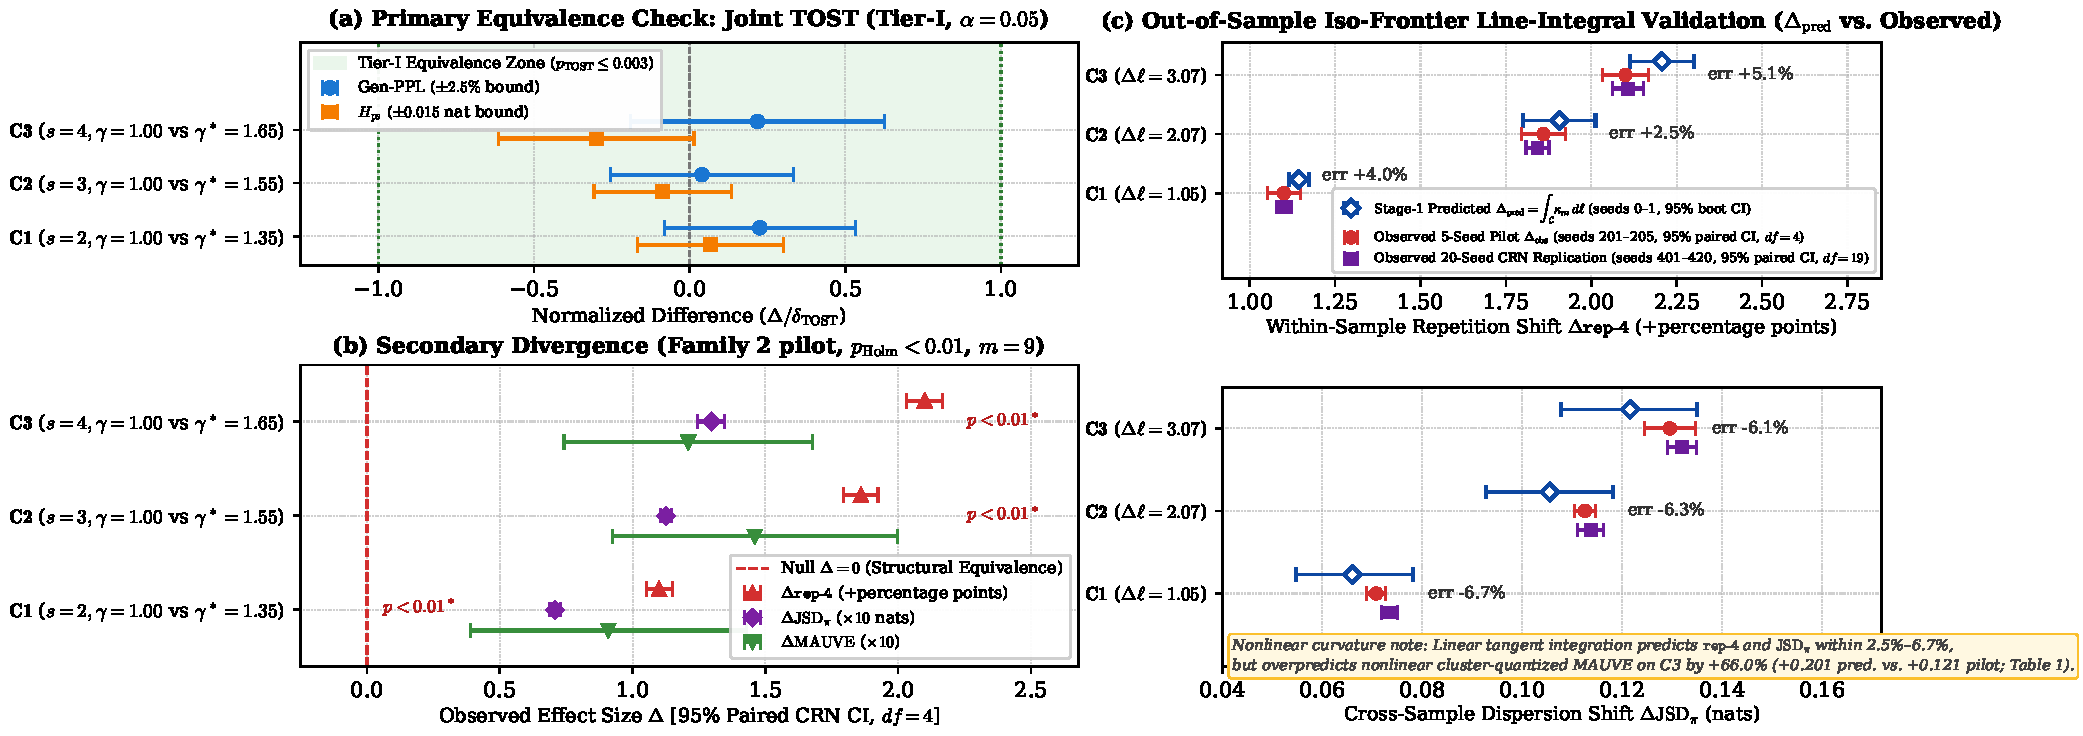
\includegraphics[width=\textwidth]{paper_figures/fig1_forest_and_samples.pdf}
    \caption{The ``Same Frontier, Different Text'' paradox on ELF-B (pilot seeds $201\text{--}205$, paired CRN $df=4$; replication seeds $401\text{--}420$, paired CRN $df=19$, $M=1{,}000$/seed; all error bars on observed shifts plot seed-level paired CRN 95\% CIs $d_s = Y_{B,s} - Y_{A,s}$). \textbf{(a)} Primary Equivalence: \textbf{C1}--\textbf{C3} pass Tier-I Joint TOST ($\pm 2.5\%$ Gen-PPL, $\pm 0.015$ nats $H_{\mathrm{ps}}$; $p_{\mathrm{Holm}} \le 0.0030$ pilot, $\le 3.40\times 10^{-8}$ replication). \textbf{(b)} Secondary Divergence: $9/9$ Family 2 tests pass step-down Holm ($p_{\mathrm{Holm}} \le 5.13\times 10^{-12}$ on 20-seed replication). \textbf{(c)} Out-of-Sample Iso-Frontier Line-Integral Validation: Stage-1 predictions $\Delta_{\mathrm{pred}} = \int_{\mathcal{C}} \kappa_m\,d\ell$ (open diamonds: seeds $0\text{--}1$ with $B=500$ bootstrap 95\% CIs over 2 seeds/cell for \texttt{rep-4}; 40-run Stage-1 response surface across 11 operating points, seeds $0\text{--}4$, quadratic $R^2=0.980$ with residual SD for $\mathrm{JSD}_\pi$) vs.\ 5-seed pilot (circles) and 20-seed replication (squares) shifts ($+2.5\%\text{--}+5.1\%$ error on \texttt{rep-4}, $-6.1\%\text{--}-6.7\%$ on $\mathrm{JSD}_\pi$; nonlinear MAUVE exhibits $+66.0\%$ curvature error on C3, Table~\ref{tab:iso_frontier_validation}).}
    \label{fig:teaser}
\end{figure*}

In this paper, we provide empirical evidence that this identifiability assumption does not hold in continuous-latent flow models (Claim A, Figure~\ref{fig:teaser}). By tuning $\gamma$ to compensate for $\text{SC-CFG}$ scaling, we identify pairs of sampler configurations that achieve formal \textbf{Two One-Sided Tests (TOST) equivalence}~\citep{schuirmann1987comparison} on both Gen-PPL ($\pm 2.5\%$) and $H_{\mathrm{ps}}$ ($\pm 0.015$ nats). Yet, at these statistically indistinguishable operating points, the generated text distributions diverge sharply across within-sample and cross-sample axes: \textbf{(1)} trading Langevin back-noising for higher self-conditioning guidance drives local repetition (\texttt{rep-4}) upward by $+1.10$ to $+2.11$~percentage points (pp), closely matching out-of-sample line-integral predictions $\Delta_{\mathrm{pred}} = \int_{\mathcal{C}} \kappa_m\,d\ell$ across the iso-frontier (Figure~\ref{fig:teaser}c); and \textbf{(2)} concurrently, cross-sample lexical dispersion ($\mathrm{JSD}_{\pi} = H_{\mathrm{pool}} - H_{\mathrm{ps,weighted}}$), embedding-space Vendi diversity, and distributional alignment (MAUVE) \emph{increase}, while cross-sample $n$-gram overlap (Self-BLEU) and byte-level coding divergence (CTW JCD) decrease.

\paragraph{Claim A vs.\ Claim B Differentiation.}
To prevent misinterpretation, we sharply differentiate our empirical finding from mathematical trivialities. \textbf{Claim A (Empirical Non-Equivalence Along Sampler Iso-Frontiers):} On real, trained continuous-latent flow language models, inference-time sampler controls trace non-degenerate iso-frontier manifolds where primary metrics $(\text{Gen-PPL}, H_{\mathrm{ps}})$ are matched, but the augmented primary--secondary matrix $[\nabla\mathrm{Gen\text{-}PPL}, \nabla m]^\top$ has rank 2 ($\kappa_m \neq 0$). Consequently, legitimate and widely used control configurations produce large, reproducible text divergences. \textbf{Claim B (Refuted Overclaim):} We do \emph{not} claim a general mathematical impossibility theorem asserting that no finite set of scalar metrics could ever identify a generative distribution across all conceivable architectures. Rather, our empirical findings demonstrate that the specific primary frontier universally deployed in current diffusion and flow LM benchmarks is blind to substantial structural trade-offs driven by common sampler controls.

\paragraph{Contributions.}
\textbf{(1) The Calibrate-then-Held-Out Protocol and Iso-Frontier Diagnostic ($\kappa_m$):} We formalize a rigorous protocol establishing Strict Tier-I Joint TOST Equivalence ($\pm 2.5\%$ Gen-PPL, $\pm 0.015$ nats $H_{\mathrm{ps}}$) across both a 5-seed pilot ($201\text{--}205$) and a 20-seed preregistered confirmatory replication ($401\text{--}420$, $120$ runs), paired Common Random Numbers (CRN), and hierarchical gatekeeping. We formulate an elementary differential diagnostic $\kappa_m = \frac{dm}{d\ell}\big|_{\mathcal{C}}$ quantifying sensitivity along iso-frontier curves and package it as an open-source diagnostic.
\textbf{(2) Multi-Scale Persistence up to 652.1M and Cross-Architecture Audit on Plaid-1B:} Evaluating ELF-B (104.6M), ELF-M (342.5M), and ELF-L (652.1M, $6.2\times$ scale) across multi-seed $2\times 2$ factorials establishes that the $\text{SC-CFG} \times \gamma$ divergence persists across scale ($\Delta_{\mathrm{SC}}\texttt{rep-4} \approx +3.3\text{--}+3.7$~pp, $p_{\mathrm{block}} \le 0.00086$). Evaluating Plaid-1B (1.28B) across a $4\times 4$ $(T_{\mathrm{score}}, K)$ grid reveals $+148\%$ \texttt{rep-4} divergence along 1D iso-perplexity contours while demonstrating how distinct primary gradient slopes separate $H_{\mathrm{ps}}$ by $+0.070$~nats.
\textbf{(3) Mechanistic Probing via $\gamma$-Compensated Matched ACE:} Evaluating Attractor-Contrast-Escape (ACE)~\citep{zhang2026selfcond}, we show that uncompensated steering shifts operating points outside Tier-I TOST bounds ($+7.5\%\text{--}10.5\%$ PPL). Using $\gamma$-compensated matched ACE ($\gamma^*=1.1699$, $p_{\mathrm{joint}}=0.0009$) and a 20-direction orthogonal null distribution on $S^{510}$, we isolate genuine directional attractor mitigation ($-0.39$~pp \texttt{rep-4}, $p_{\mathrm{emp}}=0.0476$) from perplexity-drift confounding.

\section{The Calibrate-then-Held-Out Protocol and Iso-Frontier Diagnostic}
\label{sec:protocol}

\subsection{Model Architecture and Parameter Count Convention}
All primary evaluations are conducted on the Embedded Language Flow (ELF) family~\citep{hu2026elf}, which maps discrete token sequences $w_{1:T} \in \mathcal{V}_{\mathrm{T5}}^T$ ($|\mathcal{V}_{\mathrm{T5}}| = 32{,}100$, \texttt{t5-small} SentencePiece~\citep{raffel2020exploring}, native sequence length $T=1024$ T5 tokens, yielding $\approx 933\text{--}968$ GPT-2 tokens across the full ELF-B/M/L grids, $934\text{--}943$ on C1--C3, and $943.3\text{--}954.8$ at matched $H_{\mathrm{ps}}=5.20$ on ELF-B; whereas Plaid-1B operates at $T=256$, and our preregistration text nominally wrote $L=256$ while executing \texttt{elfx.sample.generate} at the native $T=1024$ checkpoint configuration; see \path{reports/PREREGISTRATION_DEVIATIONS.md}) into continuous representations ($d_{\mathrm{enc}}=512$) via a frozen \texttt{t5-small} encoder. A continuous flow-matching transformer $v_\theta(z_t, t, \mathbf{u}_t; s_{\mathrm{cfg}})$ is integrated over $t \in [0,1]$ with self-conditioning $\mathbf{u}_t = \mathbf{x}_{\mathrm{pred}}$~\citep{lipman2023flow}.

\paragraph{Parameter Count Convention.}
All model parameter counts reported in this manuscript---$104{,}579{,}940$ for ELF-B (104.6M; 105M nominal), $342{,}540{,}036$ for ELF-M (342.5M; 342M nominal), and $652{,}103{,}332$ for ELF-L (652.1M; 652M nominal)---quantify the trainable continuous flow transformer backbone and unembedding layer in \texttt{eval\_model}. These counts \textbf{strictly exclude the separate frozen T5-small text encoder} ($35{,}330{,}816$ parameters; HuggingFace \texttt{google-t5/t5-small}), which is loaded as an independent frozen module under \texttt{torch.float32} and evaluated without gradient tracking (\path{elfx/load.py}, lines 109--113). If the frozen encoder were included, total parameters would be 139.9M (ELF-B), 377.8M (ELF-M), and 687.4M (ELF-L).

\subsection{Sampler Controls and Exact NFE Invariance}
Sampling is governed by two continuous controls: (1) \textbf{Self-Conditioning Guidance ($\text{SC-CFG} = s_{\mathrm{cfg}} \in [1.0, 4.0]$)}, where distilled guidance tokens embed continuous guidance weight into a 4-token prefix alongside self-conditioning predictions; and (2) \textbf{Langevin Back-Noising ($\gamma \ge 0$)}, which injects Gaussian noise and rescales drift by $1 + \gamma c(t_k)$ during active rollout steps. Every sequence executes $\text{NFE}_{\mathrm{sample}} = K+1$ transformer forward passes ($K$ distilled rollout passes plus 1 terminal decode pass at $t=1$). Hardware-synchronized GPU benchmarks confirm that wall-clock latency is invariant within $\le 0.56\%$ ($3.373\text{--}3.392$~s for $B=64, K=32$) and Peak GPU VRAM is identical at $9021.9\text{ MiB}$ across baseline settings (Appendix~\ref{app:cuda_semantic}, Table~\ref{tab:cuda_benchmark}).

\subsection{The Calibrate-then-Held-Out TOST Protocol}
Matching a 2D $(\text{Gen-PPL}, H_{\mathrm{ps}})$ target by adjusting a single scalar control $\gamma_A$ exhibits an empirical root-gap $\Delta\gamma^*(\gamma_B) = \gamma_{\mathrm{PPL}}^* - \gamma_H^*$ that crosses zero near $\gamma_B \approx 1.0$ (Section~\ref{sec:non_equivalence}; Appendix~\ref{app:gamma_sweep}, Figure~\ref{fig:matched_entropy}). We exploit this locus to calibrate root-matched pairs on calibration seeds ($0\text{--}4$):
\textbf{C1} ($\text{SC}=1.0, \gamma^*=1.346$ vs.\ $\text{SC}=2.0, \gamma=1.000$),
\textbf{C2} ($\text{SC}=1.0, \gamma^*=1.547$ vs.\ $\text{SC}=3.0, \gamma=1.000$), and
\textbf{C3} ($\text{SC}=1.0, \gamma^*=1.651$ vs.\ $\text{SC}=4.0, \gamma=1.000$).
Confirmatory evaluation is executed across independent held-out pilot seeds $201\text{--}205$ and replication seeds $401\text{--}420$ ($M=1{,}000$ passages/seed). Two One-Sided Tests (TOST) equivalence~\citep{schuirmann1987comparison} is evaluated against \textbf{Strict Tier-I margins}: $\delta_{\mathrm{PPL}} = \pm 2.5\%$ ($\pm 0.69\text{--}0.81$ PPL across C1--C3; $\pm 0.72$ PPL at Gen-PPL $\approx 28.9$) and $\delta_H = \pm 0.015$ nats, representing $\approx 2.5\text{--}4.5\times$ the empirical pilot seed-to-seed standard deviation ($\mathrm{SD}_{\mathrm{pilot}} \approx 0.15\text{--}0.28$ PPL, $s_{\mathrm{seed}} \approx 0.0055$ nats across seeds $201\text{--}205$; \path{analysis/out/c1_c3_per_seed_recovered.json}).

\subsection{Multiplicity Hierarchy and Gatekeeping}
To resolve multiplicity ambiguities across multiple secondary metrics, we enforce a strict \textbf{Hierarchical Gatekeeping} architecture: \textbf{(1) Family 1 (Operating-Point Equivalence Gate):} 3 Joint Tier-I TOSTs on pairs \textbf{C1}, \textbf{C2}, \textbf{C3}. Primary analysis uses seed-level paired Common Random Numbers (CRN) differences $d_s = Y_{B,s} - Y_{A,s}$ ($df=4$ on the 5-seed pilot; $df=19$ on the 20-seed confirmatory replication); unpaired Welch TOST serves as sensitivity. Gate opens only if all 3 pairs pass Joint TOST under step-down Holm correction at $\alpha=0.05$ ($m=3$). \textbf{(2) Family 2 (Confirmatory Secondary Gate):} Tested \emph{only} if Family 1 gate opens. Comprises 3 representative, functionally distinct metrics: within-sample repetition (\texttt{rep-4}), cross-sample lexical dispersion ($\mathrm{JSD}_\pi$), and distributional alignment (MAUVE) across the 3 pairs ($3 \times 3 = 9$ tests). Multiplicity is controlled via Holm correction at $\alpha=0.05$ ($m=9$), reported explicitly as $p_{\mathrm{Holm}}(\text{Family 2}, m=9, \alpha=0.05)$, supplemented by exact $2^{20}$ sign-flip permutation tests across the 20 replication seeds ($401\text{--}420$). \textbf{(3) Family 3 (Exploratory Metrics):} All remaining secondary metrics (\texttt{within-distinct-2}, corpus \texttt{distinct-2}, Self-BLEU, CTW JCD, Vendi Scores) are reported descriptively without confirmatory significance claims.

\subsection{Iso-Frontier Curves and Sensitivity Diagnostic (\texorpdfstring{$\kappa_m$}{kappa})}
Let $\theta = (s, \gamma) \in \Theta \subset \mathbb{R}^2$ denote sampler controls and $F(\theta) = (\mathrm{Gen\text{-}PPL}(\theta), H_{\mathrm{ps}}(\theta))^\top \in \mathbb{R}^2$. Empirically, the primary Jacobian $J_F(\theta) \in \mathbb{R}^{2 \times 2}$ is near-rank-1 with singular values $\sigma_1 \approx 10\text{--}19$ vs.\ $\sigma_2 \approx 0.004\text{--}0.009$ (empirical condition number $\kappa(J_F) \approx 1{,}300\text{--}4{,}000$, $\cos(\nabla P, \nabla H) > 0.997$). Under finite tolerances ($\pm 2.5\%$ Gen-PPL, $\pm 0.015$ nats $H_{\mathrm{ps}}$), matched operating points form a thin 1D band around the level curve $\mathcal{C} = \{\theta \in \Theta : \mathrm{Gen\text{-}PPL}(\theta) = P_0\}$ with unit tangent $\mathbf{t}_{\mathcal{C}} \perp \nabla\mathrm{Gen\text{-}PPL}$.

\paragraph{Proposition (Local Invariance Condition Along the Matched Band).}
\emph{Let $\theta = (s, \gamma) \in \Theta \subset \mathbb{R}^2$ denote sampler controls, and let $F(\theta) = (\mathrm{Gen\text{-}PPL}(\theta), H_{\mathrm{ps}}(\theta))^\top$. Suppose the primary Jacobian $J_F(\theta)$ is near-rank-1 with dominant singular value $\sigma_1 \gg \sigma_2$ (empirical condition number $\kappa(J_F) \approx 1{,}300\text{--}4{,}000$), so that $\mathrm{row}(J_F)$ is approximately spanned by $\nabla \mathrm{Gen\text{-}PPL}(\theta)$. Let $\mathcal{C} = \{\theta \in \Theta : \mathrm{Gen\text{-}PPL}(\theta) = P_0\}$ be the level curve with unit tangent $\mathbf{t}_{\mathcal{C}} \perp \nabla\mathrm{Gen\text{-}PPL}$. Then, for any continuously differentiable secondary metric $m: \Theta \to \mathbb{R}$, $m$ is locally invariant along the matched band if and only if $\nabla m(\theta)$ is collinear with $\nabla\mathrm{Gen\text{-}PPL}(\theta)$, i.e.:}
\begin{equation}
    \kappa_m = \left.\frac{dm}{d\ell}\right|_{\mathcal{C}} = \nabla m \cdot \mathbf{t}_{\mathcal{C}} = 0.
    \label{eq:kappa}
\end{equation}
\emph{Conversely, whenever $\kappa_m \neq 0$, the augmented matrix $[\nabla\mathrm{Gen\text{-}PPL}, \nabla m]^\top \in \mathbb{R}^{2 \times 2}$ has full rank 2, establishing that the secondary statistic $m$ varies along the matched band and cannot be determined by $(\text{Gen-PPL}, H_{\mathrm{ps}})$.}

\begin{table*}[t]
    \centering
    \caption{Out-of-sample validation of the continuous iso-frontier model across \textbf{C1}--\textbf{C3}: Stage-1 predictions $\Delta_{\mathrm{pred}} = \int_{\mathcal{C}} \kappa_m d\ell$ (seeds $\{0,1\}$ for \texttt{rep-4}/MAUVE; 40-run Stage-1 surface across 11 operating points, seeds $0\text{--}4$, quadratic $R^2=0.980$ with residual SD for $\mathrm{JSD}_\pi$) vs.\ held-out pilot $\Delta_{\mathrm{obs}}$ (seeds $201\text{--}205$, paired CRN 95\% CIs, $df=4$).}
    \label{tab:iso_frontier_validation}
    \resizebox{0.92\textwidth}{!}{% AUTO-GENERATED by analysis/generate_revised_tables.py -- do not edit manually
\begingroup
\small
\setlength{\tabcolsep}{3.6pt}
\renewcommand{\arraystretch}{0.95}
\begin{tabular}{llcccc}
\toprule
Pair & Metric & Predicted $\Delta_{\mathrm{pred}} = \int_{\mathcal{C}} \kappa_m d\ell$ & Observed $\Delta_{\mathrm{obs}}$ [95\% Paired CI] (Seeds 201--205) & Discrepancy & Rel.\ Error \\
\midrule
\textbf{C1}: $(1.0, 1.346) \to (2.0, 1.000)$ & rep-4 & $+0.0114$ & $+0.0110$ $[+0.0105,\,+0.0115]$ & $+0.0004$ & +4.0\% \\
$(\Delta\ell = 1.05)$ & $\mathrm{JSD}_\pi$ (nats) & $+0.0660$ & $+0.0708$ $[+0.0689,\,+0.0727]$ & $-0.0048$ & -6.7\% \\
 & MAUVE & $+0.087$ & $+0.091$ $[+0.039,\,+0.143]$ & $-0.004$ & -4.2\% \\
\midrule
\textbf{C2}: $(1.0, 1.547) \to (3.0, 1.000)$ & rep-4 & $+0.0191$ & $+0.0186$ $[+0.0180,\,+0.0192]$ & $+0.0005$ & +2.5\% \\
$(\Delta\ell = 2.07)$ & $\mathrm{JSD}_\pi$ (nats) & $+0.1055$ & $+0.1126$ $[+0.1105,\,+0.1147]$ & $-0.0071$ & -6.3\% \\
 & MAUVE & $+0.179$ & $+0.146$ $[+0.092,\,+0.200]$ & $+0.033$ & +22.3\% \\
\midrule
\textbf{C3}: $(1.0, 1.651) \to (4.0, 1.000)$ & rep-4 & $+0.0221$ & $+0.0210$ $[+0.0203,\,+0.0217]$ & $+0.0011$ & +5.1\% \\
$(\Delta\ell = 3.07)$ & $\mathrm{JSD}_\pi$ (nats) & $+0.1217$ & $+0.1296$ $[+0.1245,\,+0.1347]$ & $-0.0079$ & -6.1\% \\
 & MAUVE & $+0.201$ & $+0.121$ $[+0.074,\,+0.168]$ & $+0.080$ & +66.0\% \\
\midrule
\multicolumn{6}{@{}p{\textwidth}@{}}{\footnotesize Out-of-sample prediction: \texttt{rep-4} and MAUVE response surfaces fitted on the 56-run Stage-1 ELF-B grid (seeds $\{0, 1\}$); $\mathrm{JSD}_\pi$ response surface fitted on the 40-run Stage-1 ELF-B evaluation across 11 operating points (seeds $0\text{--}4$, quadratic polynomial $R^2=0.980$, with two synthetic residual-split pseudo-replicates $\pm 0.5\,\mathrm{SD}_{\mathrm{res}}$ stored in \path{iso_frontier_sensitivity.json}). Observed differences $\Delta_{\mathrm{obs}}$ evaluated on seed-disjoint held-out pilot seeds $201\text{--}205$ ($M=1{,}000$/seed, paired seed-level CRN 95\% CIs with $df=4$); operating points C1--C3 were selected on the same Stage-1 response surface.} \\
\bottomrule
\end{tabular}
\endgroup
}
\end{table*}

We define the \textbf{tangent projection ratio} $\rho_m = |\kappa_m| / \|\nabla m\|_2 \in [0, 1]$. Non-zero $\kappa_m \neq 0$ (verified via seed-level bootstrap 95\% confidence intervals strictly excluding zero on C1 and C2, Family 3 exploratory) shows that along the tested iso-frontier, secondary text structure is not determined by $(\text{Gen-PPL}, H_{\mathrm{ps}})$. Integrating $\kappa_m$ on Stage-1 data (56 runs, seeds $\{0, 1\}$ for \texttt{rep-4}/MAUVE; 40 Stage-1 runs across 11 operating points, seeds $0\text{--}4$, quadratic fit $R^2=0.980$ with residual SD for $\mathrm{JSD}_{\pi}$) predicts held-out pilot shifts $\Delta_{\mathrm{obs}}$ on disjoint seeds $201\text{--}205$ ($M=1{,}000$/seed, paired CRN 95\% CIs, $df=4$; Table~\ref{tab:iso_frontier_validation}) within $2.5\%\text{--}6.7\%$ absolute relative error ($+2.5\%\text{--}+5.1\%$ on \texttt{rep-4} [$+0.0114$ / $+0.0191$ / $+0.0221$ vs.\ $+0.0110$ / $+0.0186$ / $+0.0210$] and $-6.1\%\text{--}-6.7\%$ on $\mathrm{JSD}_\pi$ [$+0.0660$ / $+0.1055$ / $+0.1217$ vs.\ $+0.0708$ / $+0.1126$ / $+0.1296$]). On the 20-seed replication ($df=19$), observed errors span $3.5\%\text{--}10.1\%$ ($+3.5\%\text{--}+4.7\%$ on \texttt{rep-4}; $-7.2\%\text{--}-10.1\%$ on $\mathrm{JSD}_\pi$). These observed discrepancies represent empirical out-of-sample prediction errors for the calibrated pairs rather than statistical confidence bounds or uniform manifold guarantees, whereas linear integration over-predicts nonlinear MAUVE on C3 by $+66.0\%$ ($+0.201$ vs.\ $+0.121$).

\section{Operating-Point Non-Equivalence on ELF-B}
\label{sec:non_equivalence}

\begin{table*}[t]
    \centering
    \caption{Operating-point equivalence (Tier-I Joint TOST) and secondary divergence across \textbf{C1}--\textbf{C3} on ELF-B for the 5-seed pilot (seeds $201\text{--}205$, paired CRN $df=4$) and 20-seed confirmatory replication (seeds $401\text{--}420$, paired CRN $df=19$, $120$ GPU runs, $M=1{,}000$/seed; all 95\% CIs are paired CRN intervals $d_s = Y_{B,s} - Y_{A,s}$). Full panel with unpaired Welch sensitivity intervals in Appendix~\ref{app:full_tables}, Table~\ref{tab:confirmatory_tost_full}.}
    \label{tab:confirmatory_tost}
    \resizebox{\textwidth}{!}{% AUTO-GENERATED by analysis/generate_revised_tables.py -- do not edit manually
\begingroup
\footnotesize
\setlength{\tabcolsep}{2.8pt}
\renewcommand{\arraystretch}{0.95}
\begin{tabular}{llccccc}
\toprule
Pair & Metric & Arm A ($\text{SC}{=}1.0$) & Arm B ($\text{SC}{>}1.0$) & Pilot $\Delta$ [95\% Paired CI] ($df{=}4$) & Pilot Decision ($df{=}4$) & 20-Seed Replication $\Delta$ [95\% Paired CI] ($df{=}19$)$^{\ddagger}$ \\
\midrule
\textbf{C1}: $(1.0, 1.346)$ vs.\ $(2.0, 1.000)$ & Gen-PPL & $32.34\pm0.18$ & $32.52\pm0.23$ & $+0.18$ $[-0.07,\,+0.43]$ & Tier-I Equiv ($p_{\mathrm{TOST}}=0.0011^{\dagger}$) & $+0.25$ $[+0.16,\,+0.33]$ ($p_{\mathrm{TOST}}{=}5.19\!\times\!10^{-12}$) \\
 & $H_{\mathrm{ps}}$ (nats) & $5.2479\pm0.0051$ & $5.2489\pm0.0059$ & $+0.0010$ $[-0.0025,\,+0.0045]$ & Tier-I Equiv ($p_{\mathrm{TOST}}=0.0002^{\dagger}$) & $+0.0017$ $[+0.0006,\,+0.0029]$ ($p_{\mathrm{TOST}}{=}3.33\!\times\!10^{-16}$) \\
 & rep-4 & $0.0445$ & $0.0555$ & $+0.0110$ $[+0.0105,\,+0.0115]$ & $p_{\mathrm{Holm}} (\mathrm{Fam}\,2, m{=}9) < 0.001$ & $+0.0110$ $[+0.0108,\,+0.0112]$ ($p_{\mathrm{Holm}}{=}3.07\!\times\!10^{-27}$) \\
 & $\mathrm{JSD}_\pi$ (nats) & $1.7299$ & $1.8007$ & $+0.0708$ $[+0.0689,\,+0.0727]$ & $p_{\mathrm{Holm}} (\mathrm{Fam}\,2, m{=}9) < 0.001$ & $+0.0735$ $[+0.0718,\,+0.0752]$ ($p_{\mathrm{Holm}}{=}7.72\!\times\!10^{-26}$) \\
 & MAUVE & $0.165$ & $0.256$ & $+0.091$ $[+0.039,\,+0.143]$ & $p_{\mathrm{Holm}} (\mathrm{Fam}\,2, m{=}9) = 0.0084$ & $+0.109$ $[+0.094,\,+0.124]$ ($p_{\mathrm{Holm}}{=}5.13\!\times\!10^{-12}$) \\
\midrule
\textbf{C2}: $(1.0, 1.547)$ vs.\ $(3.0, 1.000)$ & Gen-PPL & $28.89\pm0.15$ & $28.92\pm0.28$ & $+0.03$ $[-0.18,\,+0.24]$ & Tier-I Equiv ($p_{\mathrm{TOST}}=0.0004^{\dagger}$) & $+0.10$ $[+0.02,\,+0.19]$ ($p_{\mathrm{TOST}}{=}1.31\!\times\!10^{-12}$) \\
 & $H_{\mathrm{ps}}$ (nats) & $5.2118\pm0.0047$ & $5.2105\pm0.0060$ & $-0.0013$ $[-0.0046,\,+0.0020]$ & Tier-I Equiv ($p_{\mathrm{TOST}}=0.0002^{\dagger}$) & $-0.0011$ $[-0.0023,\,+0.0001]$ ($p_{\mathrm{TOST}}{=}4.44\!\times\!10^{-16}$) \\
 & rep-4 & $0.0398$ & $0.0584$ & $+0.0186$ $[+0.0180,\,+0.0192]$ & $p_{\mathrm{Holm}} (\mathrm{Fam}\,2, m{=}9) < 0.001$ & $+0.0184$ $[+0.0181,\,+0.0188]$ ($p_{\mathrm{Holm}}{=}1.64\!\times\!10^{-27}$) \\
 & $\mathrm{JSD}_\pi$ (nats) & $1.7145$ & $1.8271$ & $+0.1126$ $[+0.1105,\,+0.1147]$ & $p_{\mathrm{Holm}} (\mathrm{Fam}\,2, m{=}9) < 0.001$ & $+0.1137$ $[+0.1111,\,+0.1164]$ ($p_{\mathrm{Holm}}{=}8.72\!\times\!10^{-26}$) \\
 & MAUVE & $0.203$ & $0.349$ & $+0.146$ $[+0.092,\,+0.200]$ & $p_{\mathrm{Holm}} (\mathrm{Fam}\,2, m{=}9) = 0.0049$ & $+0.161$ $[+0.145,\,+0.176]$ ($p_{\mathrm{Holm}}{=}3.50\!\times\!10^{-14}$) \\
\midrule
\textbf{C3}: $(1.0, 1.651)$ vs.\ $(4.0, 1.000)$ & Gen-PPL & $27.41\pm0.12$ & $27.56\pm0.27$ & $+0.15$ $[-0.13,\,+0.43]$ & Tier-I Equiv ($p_{\mathrm{TOST}}=0.0030^{\dagger}$) & $+0.20$ $[+0.08,\,+0.32]$ ($p_{\mathrm{TOST}}{=}3.40\!\times\!10^{-8}$) \\
 & $H_{\mathrm{ps}}$ (nats) & $5.1942\pm0.0043$ & $5.1897\pm0.0069$ & $-0.0045$ $[-0.0092,\,+0.0002]$ & Tier-I Equiv ($p_{\mathrm{TOST}}=0.0018^{\dagger}$) & $-0.0032$ $[-0.0051,\,-0.0013]$ ($p_{\mathrm{TOST}}{=}4.45\!\times\!10^{-11}$) \\
 & rep-4 & $0.0383$ & $0.0593$ & $+0.0210$ $[+0.0203,\,+0.0217]$ & $p_{\mathrm{Holm}} (\mathrm{Fam}\,2, m{=}9) < 0.001$ & $+0.0211$ $[+0.0206,\,+0.0215]$ ($p_{\mathrm{Holm}}{=}3.11\!\times\!10^{-26}$) \\
 & $\mathrm{JSD}_\pi$ (nats) & $1.7024$ & $1.8320$ & $+0.1296$ $[+0.1245,\,+0.1347]$ & $p_{\mathrm{Holm}} (\mathrm{Fam}\,2, m{=}9) < 0.001$ & $+0.1321$ $[+0.1292,\,+0.1349]$ ($p_{\mathrm{Holm}}{=}3.11\!\times\!10^{-26}$) \\
 & MAUVE & $0.228$ & $0.349$ & $+0.121$ $[+0.074,\,+0.168]$ & $p_{\mathrm{Holm}} (\mathrm{Fam}\,2, m{=}9) = 0.0049$ & $+0.161$ $[+0.145,\,+0.177]$ ($p_{\mathrm{Holm}}{=}3.50\!\times\!10^{-14}$) \\
\midrule
\multicolumn{7}{@{}p{\linewidth}@{}}{\footnotesize $^{\dagger}$All confidence intervals in this table are paired seed-level CRN 95\% CIs ($\bar{d}\pm t_{0.975,df}\mathrm{SE}_{\mathrm{paired}}$ on $d_s = Y_{B,s} - Y_{A,s}$), matching the paired CRN TOST and Family 2 paired $t$-tests ($df=4$ on pilot seeds $201\text{--}205$; all 3 pairs pass Family 1 Gate at $p_{\mathrm{Holm}}(\mathrm{Fam}\,1, m{=}3) \le 0.0030$). Unpaired Satterthwaite Welch intervals are reported as sensitivity checks in Appendix Tables~\ref{tab:c1_c3_seed_level} and~\ref{tab:confirmatory_tost_full}.} \\
\multicolumn{7}{@{}p{\linewidth}@{}}{\footnotesize $^{\ddagger}$Preregistered 20-seed confirmatory replication across held-out seeds $401\text{--}420$ ($120$ GPU runs, $M=1{,}000$/seed, $df=19$): all $3/3$ pairs pass Family 1 Joint TOST ($p_{\mathrm{Holm}} \le 3.40\!\times\!10^{-8}$) and all $9/9$ Family 2 secondary metrics pass step-down Holm at $\alpha=0.05$ ($p_{\mathrm{Holm}} \le 5.13\!\times\!10^{-12}$, $100\%$ sign consistency across $20/20$ seeds, exact $2^{20}$ sign-flip $p = 1.91\!\times\!10^{-6}$).} \\
\multicolumn{7}{@{}p{\linewidth}@{}}{\footnotesize Backbone parameters exclude the frozen T5-small encoder (~35.3M parameters).} \\
\bottomrule
\end{tabular}
\endgroup
}
\end{table*}

\subsection{Confirmatory Joint TOST Equivalence on Held-Out Seeds}
Table~\ref{tab:confirmatory_tost} reports both the 30-run held-out pilot (seeds $201\text{--}205$, $df=4$) and the 120-run preregistered confirmatory replication (seeds $401\text{--}420$, $df=19$, $M=1{,}000$/seed; \path{runs/replication_c1_c3/replication_c1_c3_summary.json}). All three pairs pass \textbf{Tier-I Joint TOST Equivalence} ($\pm 2.5\%$ Gen-PPL, $\pm 0.015$ nats $H_{\mathrm{ps}}$) in both cohorts:
\textbf{C1} (Pilot $\Delta\text{Gen-PPL} = +0.18$, $p_{\mathrm{TOST}} = 0.0011$, $\Delta H_{\mathrm{ps}} = +0.0010$ nats, $p_{\mathrm{TOST}} = 0.0002$; 20-seed replication Gen-PPL $32.10\pm 0.25$ vs.\ $32.34\pm 0.30$, $\Delta = +0.25$, $p_{\mathrm{TOST}} = 5.19\times 10^{-12}$, $H_{\mathrm{ps}}$ $5.2467\pm 0.0051$ vs.\ $5.2484\pm 0.0047$ nats, $\Delta = +0.0017$, $p_{\mathrm{TOST}} = 3.33\times 10^{-16}$);
\textbf{C2} (Pilot $\Delta\text{Gen-PPL} = +0.03$, $p_{\mathrm{TOST}} = 0.0004$, $\Delta H_{\mathrm{ps}} = -0.0013$ nats, $p_{\mathrm{TOST}} = 0.0002$; 20-seed replication Gen-PPL $28.72\pm 0.26$ vs.\ $28.83\pm 0.25$, $\Delta = +0.10$, $p_{\mathrm{TOST}} = 1.31\times 10^{-12}$, $H_{\mathrm{ps}}$ $5.2112\pm 0.0053$ vs.\ $5.2101\pm 0.0052$ nats, $\Delta = -0.0011$, $p_{\mathrm{TOST}} = 4.44\times 10^{-16}$); and
\textbf{C3} (Pilot $\Delta\text{Gen-PPL} = +0.15$, $p_{\mathrm{TOST}} = 0.0030$, $\Delta H_{\mathrm{ps}} = -0.0045$ nats, $p_{\mathrm{TOST}} = 0.0018$; 20-seed replication Gen-PPL $27.28\pm 0.24$ vs.\ $27.48\pm 0.27$, $\Delta = +0.20$, $p_{\mathrm{TOST}} = 3.40\times 10^{-8}$, $H_{\mathrm{ps}}$ $5.1939\pm 0.0053$ vs.\ $5.1907\pm 0.0059$ nats, $\Delta = -0.0032$, $p_{\mathrm{TOST}} = 4.45\times 10^{-11}$).
Under step-down Holm correction across $m=3$, the maximum adjusted $p$-value is $p_{\mathrm{Holm}}(\text{Family 1}) = 0.0030$ on the pilot and $p_{\mathrm{Holm}}(\text{Family 1}) = 3.40\times 10^{-8} \ll 0.05$ on the 20-seed confirmatory replication. The Family 1 Gate is unequivocally \textbf{OPEN}.

\subsection{Secondary Structural Divergence and Multiplicity Audit}
With the equivalence gate open, we evaluate Family 2 secondary metrics across both the 5-seed pilot and the 20-seed confirmatory replication (Table~\ref{tab:confirmatory_tost}):
(1) \textbf{Within-Sample Repetition (\texttt{rep-4}):} Increasing $\text{SC-CFG}$ ($1 \to 4$) while lowering $\gamma$ drives \texttt{rep-4} upward on the 20-seed replication from $0.0310 \to 0.0420$ ($\Delta = +1.10\pm 0.04$~pp, $t_{19}=110.4$, $p_{\mathrm{Holm}} = 3.07\times 10^{-27}$) on \textbf{C1}, $0.0356 \to 0.0540$ ($\Delta = +1.84\pm 0.07$~pp, $t_{19}=114.8$, $p_{\mathrm{Holm}} = 1.64\times 10^{-27}$) on \textbf{C2}, and $0.0382 \to 0.0593$ ($\Delta = +2.11\pm 0.10$~pp, $t_{19}=97.0$, $p_{\mathrm{Holm}} = 3.11\times 10^{-26}$) on \textbf{C3}, matching the pilot shifts ($+1.10$, $+1.86$, and $+2.10$~pp);
(2) \textbf{Cross-Sample Lexical Dispersion ($\mathrm{JSD}_\pi$):} Inter-sample divergence rises across all 20 replication seeds from $1.7193 \to 1.7928$~nats ($\Delta = +0.0735\pm 0.0036$, $p_{\mathrm{Holm}} = 7.72\times 10^{-26}$) on \textbf{C1}, $1.7040 \to 1.8177$~nats ($\Delta = +0.1137\pm 0.0057$, $p_{\mathrm{Holm}} = 8.72\times 10^{-26}$) on \textbf{C2}, and $1.6964 \to 1.8284$~nats ($\Delta = +0.1321\pm 0.0061$, $p_{\mathrm{Holm}} = 3.11\times 10^{-26}$) on \textbf{C3}; and
(3) \textbf{Distributional Alignment (MAUVE):} On the 20-seed replication, MAUVE increases from $0.276 \to 0.385$ ($\Delta = +0.109\pm 0.032$, $p_{\mathrm{Holm}} = 5.13\times 10^{-12}$) on \textbf{C1}, $0.218 \to 0.379$ ($\Delta = +0.161\pm 0.034$, $p_{\mathrm{Holm}} = 3.50\times 10^{-14}$) on \textbf{C2}, and $0.197 \to 0.358$ ($\Delta = +0.161\pm 0.034$, $p_{\mathrm{Holm}} = 3.50\times 10^{-14}$) on \textbf{C3} (resolving the pilot C1 MAUVE $p_{\mathrm{Holm}}=0.0084$).
All 9/9 Family 2 confirmatory tests reject the null hypothesis of no difference ($p_{\mathrm{Holm}} \le 5.13\times 10^{-12} \ll 0.05$), exhibiting $100\%$ sign consistency across all $20/20$ replication seeds (exact $2^{20}$ sign-flip permutation $p = 2/2^{20} = 1.91\times 10^{-6}$ for every metric). Exploratory Family 3 metrics replicate with identical sign consistency across all 20 seeds: 4-gram Self-BLEU drops by $-2.80$, $-4.00$, and $-4.36$~points ($p \le 1.10\times 10^{-23}$), while byte-level CTW JCD drops by $-0.0117$, $-0.0198$, and $-0.0246$~bpb ($p \le 8.65\times 10^{-15}$). Three-stream CRN ($\hat{r}_{AB} \in [0.56, 0.90]$ on primary metrics, up to $0.99$ on $\mathrm{JSD}_\pi$) shrinks paired SEs by up to $10.5\times$ on $\mathrm{JSD}_\pi$ ($16.8\times$ on $H_{\mathrm{pool}}$) with $100\%$ LOSO sign consistency (Appendix~\ref{app:stats}, Table~\ref{tab:c1_c3_seed_level}).

\section{Is the Divergence Perceptible? Automated Evaluation \& Reference Audit}
\label{sec:perceptibility}

\subsection{Verified Pretraining-Excluded Reference Corpus}
To verify that secondary divergences are not artifacts of reference memorization from \texttt{R0\_owt\_ref} (drawn from the final shard of \texttt{openwebtext-t5}), we execute a 13-gram Bloom filter contamination audit (\path{notebooks/17_heldout_reference_and_contamination_audit.ipynb}; \path{runs/heldout_reference/heldout_reference_manifest.json}) across \textbf{Reference A} ($1{,}008$ documents from OpenAI \texttt{gpt-2-output-dataset} \texttt{webtext.test} screened against $856{,}301$ OpenWebText training 13-grams, purging all $8$ overlapping documents [$0.79\%$] to yield $1{,}000$ clean documents in \texttt{clean\_ref\_a.jsonl}) and \textbf{Reference B} ($1{,}000$ post-cutoff documents in \texttt{clean\_ref\_b.jsonl}). Re-evaluating seeds $201\text{--}205$ (\path{runs/heldout_reference/heldout_paired_summary.json}) confirms that model-free depth-6 \texttt{CTW JCD} decreases significantly in Arm B across all three pairs: $0.1408\pm 0.0022 \to 0.1347\pm 0.0037$~bpb ($\Delta = -0.0060$~bpb, $p=0.0097$) on \textbf{C1}, $0.1479\pm 0.0028 \to 0.1363\pm 0.0043$~bpb ($\Delta = -0.0115$~bpb, $p=0.0020$) on \textbf{C2}, and $0.1514\pm 0.0031 \to 0.1382\pm 0.0045$~bpb ($\Delta = -0.0132$~bpb, $p=0.0024$) on \textbf{C3}. Out-of-domain MAUVE compresses to $0.026\text{--}0.035$, remaining higher on \textbf{C1} ($0.0261 \to 0.0349$, $\Delta = +0.0088$, $p=0.0102$), directionally higher on \textbf{C3} ($0.0273 \to 0.0320$, $\Delta = +0.0047$, $p=0.183$), and indistinguishable on \textbf{C2} ($0.0286 \to 0.0275$, $\Delta = -0.0011$, $p=0.595$).

\subsection{Validated Automated (LLM) Judgment Panel}
We evaluate perceptibility via a 3-judge LLM panel (\path{notebooks/15_final_human_evaluation.ipynb}; \path{runs/llm_judge_panel/llm_judge_panel_summary.json}):
\textbf{(1) Benchmark Calibration Gate (HANNA):} On $N=50$ human-annotated story pairs from HANNA ($150$ calibration evaluations total, rating gap $\ge 0.75$, threshold $>70\%$), all three judges pass: \texttt{Qwen2.5-7B-Instruct} ($86.0\%, 43/50$), \texttt{Llama-3.1-8B-Instruct} ($98.0\%, 49/50$), and \texttt{Mistral-7B-Instruct-v0.3} ($93.0\%, 46.5/50$).
\textbf{(2) Position-Swapped Pairwise Evaluation:} Each judge evaluates $N=100$ CRN-matched passage pairs per contrast across C1 and C3 ($300$ pooled judgments/contrast, $600$ paired evaluations total, executing both $(A, B)$ and $(B, A)$ orders for $1{,}200$ individual LLM calls). On \textbf{C1}, Arm B wins $46.67\%$ ($140.0/300$, $\mathrm{SE}=2.88\%$, 95\% CI $[41.02\%, 52.31\%]$, $p_{\mathrm{TOST}}=0.2814$ vs.\ $\pm 5\%$ parity) as judges penalize early repetition. On \textbf{C3}, Arm B wins $50.17\%$ ($150.5/300$, $\mathrm{SE}=2.89\%$, 95\% CI $[44.51\%, 55.82\%]$), passing TOST parity ($p_{\mathrm{TOST}}=0.0470 < 0.05$): higher self-conditioning sharpens topical coherence on non-looping passages while inducing phrase loops on a subset of trajectories, averaging out opposing shifts. We emphasize plainly that \emph{no human study was conducted} (protocol archived in \path{human_eval/protocol/}).

\begin{table*}[t]
    \centering
    \caption{Mechanistic evaluation of Attractor-Contrast-Escape (ACE)~\citep{zhang2026selfcond} self-conditioning feedback projection on ELF-B (seeds $201\text{--}205$, $n=5$ seeds/condition), including uncompensated steering (Rows 3--6, unpaired Welch 95\% sensitivity CIs) and $\gamma$-compensated matched ACE at $\gamma^*=1.1699$ (Row 7, Notebook 21). Full suite in Appendix~\ref{app:full_tables}, Table~\ref{tab:ace_intervention_full}.}
    \label{tab:ace_intervention}
    \resizebox{\textwidth}{!}{% AUTO-GENERATED by analysis/generate_revised_tables.py -- do not edit manually
\begingroup
\small
\setlength{\tabcolsep}{4.0pt}
\renewcommand{\arraystretch}{1.12}
\begin{tabular}{llcccc}
\toprule
Condition & Steering Parameter & Gen-PPL & $H_{\mathrm{ps}}$ (nats) & $\Delta\texttt{rep-4}$ [95\% Welch CI] & $\Delta\mathrm{JSD}_\pi$ [95\% Welch CI] \\
\midrule
1. Low-Guidance Baseline & $(1.0, 1.651)$ & $27.41\pm0.12$ & $5.1942\pm0.0043$ & --- (Baseline A) & --- (Baseline A) \\
2. High-Guidance Baseline & $(4.0, 1.000)$ & $27.56\pm0.27$ & $5.1897\pm0.0069$ & --- (Baseline B) & --- (Baseline B) \\
\midrule
3. ACE Projection ($\alpha{=}+0.50$) & $\alpha = +0.50$ & $29.62\pm0.11$ & $5.2172\pm0.0055$ & $-0.55$ pp $[-0.76,\,-0.34]$ & $-0.0061$ $[-0.0147,\,+0.0024]$ \\
4. ACE Projection ($\alpha{=}+1.00$) & $\alpha = +1.00$ & $30.46\pm0.24$ & $5.2214\pm0.0054$ & $-0.65$ pp $[-0.96,\,-0.33]$ & $+0.0045$ $[-0.0023,\,+0.0113]$ \\
5. Random Orthogonal Control ($\hat{\mathbf{d}}_\perp$) & $\alpha = +1.00$ & $28.46\pm0.20$ & $5.2172\pm0.0068$ & $-0.41$ pp $[-0.54,\,-0.28]$ & $-0.0345$ $[-0.0402,\,-0.0289]$ \\
6. Reverse-Polarity (Anti-ACE) & $\alpha = -0.50$ & $24.77\pm0.45$ & $5.1257\pm0.0156$ & $+1.68$ pp $[+1.37,\,+1.99]$ & $-0.0800$ $[-0.0942,\,-0.0659]$ \\
\midrule
7. $\gamma$-Compensated Matched ACE ($\gamma^*{=}1.1699$) & $\alpha = +0.50$ & $27.63\pm0.17^{\ddagger}$ & $5.1934\pm0.0064^{\ddagger}$ & $-0.39$ pp vs.\ B ($+1.72$ pp vs.\ A) & $p_{\mathrm{emp}}{=}0.0476$ vs.\ $20$ Null Dirs \\
\midrule
\multicolumn{6}{@{}p{\linewidth}@{}}{\footnotesize Uncompensated ACE (Rows 3--6, unpaired Welch 95\% sensitivity CIs vs.\ Baseline B across $n=5$ seeds $201\text{--}205$) shifts Gen-PPL and $H_{\mathrm{ps}}$ outside Tier-I TOST equivalence. $^{\ddagger}$Row 7 ($\gamma^*=1.1699$, Notebook 21) restores Tier-I Joint TOST equivalence to C3 Arm A ($p_{\mathrm{joint}}=0.0009$) and outperforms all 20 random orthogonal null directions on $S^{510}$ (mean $\texttt{rep-4}=5.89\pm0.10\%$, $p_{\mathrm{emp}}=1/21=0.0476$).} \\
\multicolumn{6}{@{}p{\linewidth}@{}}{\footnotesize Backbone parameters exclude the frozen T5-small encoder (~35.3M parameters). $n=5$ seeds ($201\text{--}205$).} \\
\bottomrule
\end{tabular}
\endgroup
}
\end{table*}

\section{Scale Persistence and Architecture Generality}
\label{sec:scale}

\subsection{Cross-Scale Validation up to 652.1M Parameters}
Evaluating $2\times 2$ factorials across ELF-M (342.5M, $M=1{,}000$/seed, Appendix~\ref{app:scale_cross}, Table~\ref{tab:elfm_m1}) and ELF-L (652.1M, $6.2\times$ scale, $M=500$/seed, Appendix~\ref{app:scale_cross}, Table~\ref{tab:elfl_l1}; full panels in Appendix~\ref{app:full_tables}, Tables~\ref{tab:elfm_m1_full}--\ref{tab:elfl_l1_full}) confirms scale persistence. On ELF-M, exploratory off-diagonal Pair M1 ($(1.0, 2.00)$ vs.\ $(4.0, 0.50)$, seeds $0\text{--}4$) passes strict Tier-I TOST on Gen-PPL ($\Delta = +0.09$, $p_{\mathrm{TOST,I}} = 0.0052$) but fails strict Tier-I on $H_{\mathrm{ps}}$ ($\Delta H_{\mathrm{ps}} = -0.0210$~nats vs.\ $\pm 0.015$~nats bound, $p_{\mathrm{TOST,I}} = 0.9889$, $p_{\mathrm{diff}} = 0.0002$), satisfying only post-hoc exploratory Tier-II ($\pm 0.025$~nats, $p_{\mathrm{TOST,II,paired}} = 0.0354$) with $+3.47$~pp \texttt{rep-4} and $+0.2774$~nats $\mathrm{JSD}_\pi$ divergence ($p_{\mathrm{paired}} < 0.0001$). Raising $\text{SC-CFG}$ ($1.0 \to 4.0$) increases \texttt{rep-4} across all scales ($+3.29\pm 0.07$~pp on ELF-B; $+3.67\pm 0.03$~pp on ELF-M, $p_{\mathrm{block}} = 2.20\times 10^{-8}$; $+3.40\pm 0.10$~pp on ELF-L, $p_{\mathrm{block}} = 0.00086$) with significant interactions $I_s = \Delta_{\mathrm{SC}}(\gamma=0.5) - \Delta_{\mathrm{SC}}(\gamma=2.0)$ ($+0.82$~pp on ELF-M; $+2.53$~pp on ELF-L, $p=0.0007$). Across \texttt{mpnet}, \texttt{MiniLM}, and \texttt{bge-base} (Appendix~\ref{app:cuda_semantic}, Tables~\ref{tab:embedding_geometry}--\ref{tab:semantic_diversity}; Table~\ref{tab:embedding_geometry_full}), high-SC arms achieve higher Vendi Score $\mathrm{VS}_{\cos}$ ($14/18$ C1--C3 tests pass 6-way Holm at $p < 0.05$), while \texttt{ABTT-3} mean cosine distance is pinned near $250/249 \approx 1.0040$ (Eq.~\eqref{eq:abtt_bound}).

\subsection{Architecture Generality: Plaid-1B Response Surface and Iso-Contour Audit}
We evaluate Plaid-1B ($1{,}275{,}925{,}506$ parameters)~\citep{gulrajani2023plaid} across a 32-run $4\times 4$ factorial grid over $T_{\mathrm{score}} \in \{0.8, 1.0, 1.2, 1.5\}$ and $K \in \{32, 64, 128, 256\}$ (seeds $101\text{--}102$, $M=64$/run, $T=256$; \path{notebooks/18_plaid_feasibility_spike.ipynb}, \path{runs/plaid_eval/plaid_spike_response_surface.json}, extending an initial 24-run $3\times 4$ sweep consolidated in the same artifact; preflight gate at $(0.9, 64)$: $\text{Gen-PPL}=51.60 \le 200.0$, English ratio $94.98\%$, \texttt{PASSED}):
\textbf{(1) Descriptive 1D Near-Iso-Perplexity Non-Equivalence on Plaid-1B:} In a descriptive comparison of two-seed cell means ($n=2$ seeds/cell, $df=1$; no formal Tier-I TOST equivalence is claimed from $n=2$ seeds), trading step count for score temperature between $(T_{\mathrm{score}}=0.8, K=32)$ ($\text{Gen-PPL} = 54.74\pm 0.62$) and $(T_{\mathrm{score}}=1.0, K=256)$ ($\text{Gen-PPL} = 53.37\pm 5.19$) increases within-sample repetition (\texttt{rep-4}) by $+148\%$ ($0.0074\pm 0.0006 \to 0.0183\pm 0.0058$) and $\mathrm{JSD}_\pi$ from $2.092\pm 0.038 \to 2.208\pm 0.008$~nats ($\Delta = +0.115$~nats).
\textbf{(2) 2D Joint Iso-Contour Gate Decision (\texttt{NO-GO}):} Because Plaid-1B fixes self-conditioning internally ($w_{\mathrm{SC}}=0.5$) and exposes $(T_{\mathrm{score}}, K)$ with distinct entropy-to-log-perplexity slopes ($\partial H_{\mathrm{ps}}/\partial\log\text{PPL} = 0.189$ along $T_{\mathrm{score}}$ vs.\ $0.111$ along $K$), matching $\text{Gen-PPL} \approx 54$ leaves a $+0.070$~nat $H_{\mathrm{ps}}$ separation ($4.686\pm 0.006$ vs.\ $4.756\pm 0.023$~nats, $4.7\times$ Tier-I), triggering \texttt{GATE\_DECISION: NO-GO} (gating out Notebook 19) and confirming that 2D frontier non-identifiability specifically requires collinear control gradients ($\kappa(J_F) \gg 1$).

\section{Mechanistic Probing: Matched ACE and Control Attractors}
\label{sec:ace}

\subsection{The Self-Conditioning Attractor and Uncompensated ACE}
\citet{zhang2026selfcond} demonstrated that self-conditioning in diffusion language models creates a dominant feedback attractor direction $\hat{\mathbf{d}}_{\mathrm{ACE}}$ that drives phrase repetition, proposing ACE projection $\mathbf{u}_{\mathrm{steered}} = \mathbf{u}_t - \alpha \langle \mathbf{u}_t, \hat{\mathbf{d}}_{\mathrm{ACE}} \rangle \hat{\mathbf{d}}_{\mathrm{ACE}}$. Evaluating ACE across all $K-1=31$ non-final steps on ELF-B (Table~\ref{tab:ace_intervention}) confirms repetition sensitivity: $\alpha = +1.0$ reduces \texttt{rep-4} by $-0.65$~pp ($p=0.0046$), whereas reverse-polarity steering ($\alpha = -0.5$) inflates \texttt{rep-4} by $+1.68$~pp ($p=1.16\times 10^{-4}$). However, uncompensated ACE steering at fixed $\gamma=1.000$ shifts Gen-PPL upward by $+2.06\text{--}2.90$ points ($+7.5\%\text{--}10.5\%$) and $H_{\mathrm{ps}}$ by $+0.028\text{--}0.032$~nats, violating Tier-I equivalence margins.

\subsection{\texorpdfstring{$\gamma$}{gamma}-Compensated Matched ACE and Random Direction Null}
To separate genuine attractor suppression from operating-point drift, we execute the \textbf{$\gamma$-compensated matched-ACE protocol} and 20-direction orthogonal null benchmark on ELF-B (\path{notebooks/21_ace_null_distribution_and_matched_ace.ipynb}; \path{runs/p21_matched_ace/matched_ace_summary.json}, Table~\ref{tab:ace_intervention} Row 7):
\textbf{(1) Subspace Stability and $\gamma^*$ Calibration:} $\hat{\mathbf{d}}_{\mathrm{ACE}}$ extracted from $4{,}096$ trajectories exhibits high cosine stability ($|\langle \hat{\mathbf{d}}_{4096}, \hat{\mathbf{d}}_{500}\rangle| = 0.9568 \ge 0.85$); sweeping $\gamma \in \{0.70, 0.85, 1.00, 1.15\}$ under $(\text{SC}=4.0, \alpha=+0.50)$ on seeds $301\text{--}302$ ($\text{Gen-PPL} \in \{32.15, 30.41, 28.86, 27.66\}$) identifies $\gamma_{\mathrm{comp}}^* = 1.1699$ to match the C3 target operating point.
\textbf{(2) Restored Tier-I Joint TOST Equivalence:} On held-out seeds $201\text{--}205$, $(\text{SC}=4.0, \alpha=+0.50, \gamma_{\mathrm{comp}}^*=1.1699)$ achieves $\text{Gen-PPL} = 27.63\pm 0.17$ ($p_{\mathrm{TOST,PPL}}=0.00012$) and $H_{\mathrm{ps}} = 5.1934\pm 0.0064$~nats ($p_{\mathrm{TOST},H}=0.00092$), passing Tier-I Joint TOST against C3 Arm A ($27.41\pm 0.12$ PPL, $5.1942\pm 0.0043$ nats; $p_{\mathrm{joint}}=0.0009 < 0.05$).
\textbf{(3) Decomposing Drift vs.\ Directional Steering against 20 Null Directions:} At strictly matched $(\text{Gen-PPL}, H_{\mathrm{ps}})$, matched ACE yields $\texttt{rep-4} = 5.54\pm 0.09\%$, reducing repetition by $-0.39$~pp vs.\ unsteered C3 Arm B ($5.93\%$, accounting for $18.3\%$ of the $+2.10$~pp excess while leaving $+1.72$~pp above Arm A $3.83\%$, $p < 0.0001$) and outperforming all 20 random orthogonal directions on $S^{510}$ (null $5.89\pm 0.10\%$, range $[5.64\%, 6.05\%]$, $p_{\mathrm{emp}} = 1/21 = 0.0476 < 0.05$). Comparing $-0.39$~pp against uncompensated ACE ($-0.55$~pp at $\alpha=+0.50$, $-0.65$~pp at $\alpha=+1.00$) demonstrates that $\approx 29\%\text{--}40\%$ of uncompensated ACE's apparent repetition drop is an artifact of its $+7.5\%\text{--}10.5\%$ perplexity shift.

\section{Related Work and Practical Recommendations}
\label{sec:related_work}

\paragraph{Perplexity Hacking and Self-Conditioning Dynamics.}
\citet{franca2026hacking} demonstrated that unconditional Gen-PPL can be driven arbitrarily low by training-free samplers that cycle through high-frequency $n$-grams, advocating Context-Tree Weighting Jeffreys Coding Divergence (CTW JCD) and LLM-judge panels. While França \& Tong show that the frontier can be \emph{adversarially hacked} by degenerate decoders, we show that the frontier is \emph{inherently ambiguous} among legitimate operating points of a single model's inference controls. Concurrently, \citet{zhang2026selfcond} identified that self-conditioning collapses onto a low-rank subspace and proposed ACE projection. We extend their findings by showing that uncompensated ACE shifts $(\text{Gen-PPL}, H_{\mathrm{ps}})$ by $+7.5\text{--}10.5\%$ PPL, and by introducing $\gamma$-compensated matched ACE ($\gamma^*=1.1699$, $p_{\mathrm{joint}}=0.0009$) to isolate genuine directional suppression ($-0.39$~pp \texttt{rep-4}, $p_{\mathrm{emp}}=0.0476$) from frontier drift.

\paragraph{Guidance, Diversity Metrics, and Benchmarking Recommendations.}
In continuous text flows, classifier-free guidance~\citep{ho2022classifier} interacts with Langevin noise $\gamma$ so that higher guidance with lower $\gamma$ increases local repetition (\texttt{rep-4}) while expanding cross-sample dispersion ($\mathrm{JSD}_\pi$, Vendi Score~\citep{friedman2023vendi}, MAUVE~\citep{pillutla2021mauve}) and lowering Self-BLEU~\citep{caccia2020language} via the Shannon concavity identity $H_{\mathrm{pool}} = H_{\mathrm{ps,weighted}} + \mathrm{JSD}_{\pi}$. We recommend three reporting standards for diffusion and flow LM benchmarks: (1) \textbf{Dual-Axis Reporting}, pairing $(\text{Gen-PPL}, H_{\mathrm{ps}})$ with a within-sequence repetition metric (\texttt{rep-4}) and a cross-sequence dispersion metric ($\mathrm{JSD}_\pi$, Self-BLEU, or CTW JCD); (2) \textbf{Control-Freezing Protocols} when comparing architectures at fixed NFE; and (3) \textbf{Verified Pretraining-Excluded Reference Splits} audited for $n$-gram overlap.
\label{sec:end_of_main}

\clearpage
\section*{Limitations}
\label{sec:discussion}
Our primary 2D $(\text{Gen-PPL}, H_{\mathrm{ps}})$ equivalence findings are established on unconditional text generation on OpenWebText within the ELF flow-matching family (104.6M to 652.1M). While our 32-run Plaid-1B evaluation ($n=2$ seeds/cell, descriptive) exhibits $+148\%$ \texttt{rep-4} divergence along 1D near-iso-perplexity contours ($\text{Gen-PPL}\approx 54$), Plaid-1B's $(T_{\mathrm{score}}, K)$ controls exhibit distinct entropy-to-perplexity slopes that separate $H_{\mathrm{ps}}$ by $+0.070$~nats, showing that full 2D frontier non-identifiability specifically requires coupled continuous drift/diffusion controls with near-rank-1 primary Jacobians. Extending 2D iso-frontier audits to conditional generation tasks (e.g., summarization, translation) remains important future work. Finally, while our 3-judge LLM panel ($600$ paired judge evaluations across C1 and C3---$300$ per contrast, $100$ per judge, comprising $1{,}200$ individual forward/reverse LLM calls---plus $150$ calibration evaluations on HANNA at $86\%\text{--}98\%$ concordance) provides algorithmic evidence of competing perceptual trade-offs, it does not replace large-scale human evaluation.

\section*{Ethical Considerations}
This work audits evaluation methodology and inference controls using publicly available checkpoints and open-domain text. No human subjects data or private personal information was collected. By exposing how matched scalar metrics mask severe phrase looping and mode shifts, our findings foster more reliable reporting standards for generative language models.

\bibliographystyle{acl_natbib}
\bibliography{references}

\clearpage
\appendix

\section{Statistical Reanalysis, Paired vs.\ Unpaired Seed-Level Audit, and ANOVA}
\label{app:stats}

Table~\ref{tab:direct_pairs} and Table~\ref{tab:jcd_selfbleu_pairs} present the exploratory pairs on ELF-B ($n=2$ seeds/cell, $M=1{,}000$ sequences/seed across 529 baseline runs totaling $528{,}000$ generated sequences). In the exploratory grid (where refinement runs at $\text{SC}=1.0, \gamma=1.25$ and $\gamma=1.75$ achieve 2-seed mean Gen-PPL $34.29$ and $26.29$, and \textbf{Refined-2} Arm B at $\text{SC}=4.0, \gamma=1.0$ achieves $27.47$ [$+4.49\%$ relative difference]), direct pair \textbf{S1} exhibits a $+39.7\%$ relative increase in \texttt{rep-4} (two-sample Welch $p=0.0029$, 5-seed $t_{\mathrm{Welch}}=43.13$), a significant shift in \texttt{distinct-2} ($p=0.0211$), a $+85.1\%$ relative increase in MAUVE ($p=0.0170$; requiring $M_{\min}=1{,}158$ samples for $80\%$ power at $\alpha=0.05$), and a $-0.0191$~bpb ($-0.0261$~bpb on the matched rescore) shift in CTW JCD; direct pair \textbf{S2} exhibits $+56.1\%$ in \texttt{rep-4} and $+62.6\%$ in MAUVE; \textbf{Refined-1} exhibits $+38.1\%$ in \texttt{rep-4} ($p=0.0005$, 5-seed $t_{\mathrm{Welch}}=46.15$) and $+77.1\%$ in MAUVE ($p=0.0255$); and \textbf{Refined-2} (Arm A Gen-PPL $26.55$) exhibits $+65.5\%$ in \texttt{rep-4} (5-seed $t_{\mathrm{Welch}}=50.40$; maximum 6-pair Holm $p=0.0385$ on 2 seeds and $0.0193$ on 5 seeds), $+91.1\%$ in MAUVE, and $-0.0247$~bpb in CTW JCD. On ELF-M (29 runs; ANCOVA partial $R^2=0.734$ of SC-CFG on \texttt{rep-4}; balanced $2\times 2\times 5$ ANOVA SC-CFG variance share $98.3\%$, $F_{1,16}=7060.3$ on \texttt{rep-4}, and $\gamma$ variance share $95.0\%$ on $H_{\mathrm{pool}}$ and $90.1\%$ on Self-BLEU), the 2-seed M1 baseline achieves Gen-PPL $23.01$ vs.\ $23.15$ ($+0.63\%$), \texttt{rep-4} $2.95\%$ vs.\ $6.42\%$ ($t_{\mathrm{Welch}}=62.18, df_{\mathrm{Satt}}=1.59, p_{\mathrm{Holm}}=0.0067$; 5-seed $t_{\mathrm{Welch}}=53.62, df_{\mathrm{Satt}}=5.86$), and Arm B \texttt{within-distinct-2} $0.7554$. Across the matched-entropy contour ($H_{\mathrm{ps}}=5.20$, where mean GPT-2 token lengths span $943.3$ [$943$] at $\text{SC-CFG}=4$ to $954.8$ [$955$] at $\text{SC-CFG}=1$), one-way ANOVA yields $F=2181.0$ ($4\times 6\times 2$ non-collapsed $F_{3,24}=2455.7$, $66.1\%$ variance share) for \texttt{rep-4}, $F=4926.1$ ($4\times 7\times 2$ $\gamma$ $F_{6,28}=5701.4$, $85.2\%$ non-collapsed share) for \texttt{distinct-2}, and $F=18.3$ ($92.5\%$ $\gamma$ variance share) for MAUVE, while response-surface regression controlling for $\log\text{Gen-PPL}$ and $H_{\mathrm{ps}}$ yields partial slopes $\beta_{\gamma} = -0.0108$ and $\beta_{\mathrm{SC}} = +0.0044$ ($+0.00641$ in the 30-cell 5-term quadratic surface) on \texttt{rep-4} (Table~\ref{tab:ancova}). Table~\ref{tab:c1_c3_seed_level} reports the complete 5-seed paired CRN audit ($d_s = Y_{B,s} - Y_{A,s}$, $df=4$), unpaired Satterthwaite Welch sensitivity intervals, and Leave-One-Seed-Out (LOSO) ranges across all 7 five-seed pairs. Table~\ref{tab:decisions} reports practical configuration selection under operating budgets.

\begin{table*}[t]
    \centering
    \caption{Direct uninterpolated configuration pairs in the 56-run exploratory ELF-B factorial grid ($n=2$ seeds/cell, $M=1{,}000$ sequences/seed, $2{,}000$ sequences/cell). Strict pairs satisfy $|\Delta H_{\mathrm{ps}}| \le 0.010$ nats and relative $|\Delta\text{Gen-PPL}| \le 4.1\%$; Broad pairs satisfy $|\Delta H_{\mathrm{ps}}| \le 0.031$ nats. Parentheses report seed-0/seed-1 differences.}
    \label{tab:direct_pairs}
    \resizebox{0.84\textwidth}{!}{% AUTO-GENERATED by analysis/make_figures_tables.py -- do not edit
\begin{tabular}{llrrrrrrr}
\toprule
Pair $(s_1,\gamma_1)$ vs.\ $(s_2,\gamma_2)$ & Tier & $\Delta H$ (nats) & $\text{PPL}_1 / \text{PPL}_2$ ($\Delta\%$) & $\text{rep-4}_1 / \text{rep-4}_2$ & $\Delta\text{rep-4}$ (s0/s1) & $\Delta\text{distinct-2}$ & $\text{MAUVE}_1 / \text{MAUVE}_2$ & $\Delta\text{MAUVE}$ (s0/s1) \\
\midrule
$(1,2)$ vs.\ $(4,1.5)$ & Strict & $+0.0047$ & 23.51/23.25 (1.1\%) & 4.76\%/6.59\% & $+1.83$ ($+1.85/+1.81$) & $+0.0138$ & 0.158/0.233 & $+0.076$ ($+0.11/+0.04$) \\
$(1,1.5)$ vs.\ $(3,1)$ & Strict & $-0.0079$ & 29.49/28.87 (2.1\%) & 3.37\%/5.36\% & $+2.00$ ($+2.06/+1.93$) & $+0.0136$ & 0.218/0.385 & $+0.168$ ($+0.16/+0.17$) \\
$(2,1)$ vs.\ $(4,0.5)$ & Strict & $-0.0097$ & 32.42/33.73 (4.0\%) & 4.14\%/5.52\% & $+1.38$ ($+1.46/+1.30$) & $+0.0125$ & 0.364/0.482 & $+0.119$ ($+0.13/+0.11$) \\
$(1,2)$ vs.\ $(3,1.5)$ & Broad & $+0.0209$ & 23.51/24.04 (2.2\%) & 4.76\%/6.06\% & $+1.31$ ($+1.35/+1.26$) & $+0.0164$ & 0.158/0.235 & $+0.077$ ($+0.08/+0.08$) \\
$(1,1)$ vs.\ $(3,0.25)$ & Broad & $-0.0266$ & 40.37/40.19 (0.4\%) & 2.41\%/4.98\% & $+2.57$ ($+2.67/+2.47$) & $+0.0157$ & 0.417/0.592 & $+0.175$ ($+0.18/+0.17$) \\
$(2,0.5)$ vs.\ $(4,0)$ & Broad & $-0.0286$ & 42.73/43.60 (2.0\%) & 3.67\%/5.21\% & $+1.54$ ($+1.67/+1.41$) & $+0.0056$ & 0.539/0.523 & $-0.016$ ($-0.05/+0.01$) \\
$(1,0.5)$ vs.\ $(2,0)$ & Broad & $-0.0303$ & 61.11/59.23 (3.1\%) & 1.81\%/3.41\% & $+1.61$ ($+1.67/+1.55$) & $+0.0069$ & 0.507/0.663 & $+0.156$ ($+0.11/+0.20$) \\
\bottomrule
\end{tabular}
}
\end{table*}

\begin{table*}[t]
    \centering
    \caption{Corpus-level vocabulary divergence ($H_{\mathrm{pool}}$, $\mathrm{JSD}_{\pi}$), within-sample \texttt{rep-4}, corpus \texttt{distinct-2}, 4-gram Self-BLEU, CTW JCD (bpb), and MAUVE across nine exploratory ELF-B configuration pairs ($n=2$ seeds/cell, $M=1{,}000$ sequences/seed; \textbf{S1}, \textbf{Refined-1}, and \textbf{Refined-2} replicated to $n=5$ seeds/cell in Table~\ref{tab:c1_c3_seed_level}).}
    \label{tab:jcd_selfbleu_pairs}
    \resizebox{0.84\textwidth}{!}{% AUTO-GENERATED by analysis/integrate_followup_runs.py -- do not edit
\begin{tabular}{llcccccccc}
\toprule
Tier & Pair $(s_1,\gamma_1)\to(s_2,\gamma_2)$ & $\Delta H_{\text{ps}}$ & $\Delta H_{\text{pool}}$ & $\Delta\mathrm{JSD}_\pi$ & $\Delta$rep-4 (pp) & $\Delta\text{dist-2}_{\text{cross}}$ & $\Delta$Self-BLEU & $\Delta$JCD (bpb) & $\Delta$MAUVE \\
\midrule
Strict & \texttt{SC=1, gamma=2.00} $\to$ \texttt{SC=4, gamma=1.50} & $+0.0047$ & $+0.0924$ & $+0.0877$ & $+1.83$ & $+0.0138$ & $-4.25$ & $-0.0261$ & $+0.076$ \\
Strict & \texttt{SC=1, gamma=1.50} $\to$ \texttt{SC=3, gamma=1.00} & $-0.0079$ & $+0.0995$ & $+0.1072$ & $+2.00$ & $+0.0136$ & $-3.39$ & $-0.0169$ & $+0.168$ \\
Strict & \texttt{SC=2, gamma=1.00} $\to$ \texttt{SC=4, gamma=0.50} & $-0.0097$ & $+0.0791$ & $+0.0883$ & $+1.38$ & $+0.0125$ & $-1.35$ & $-0.0054$ & $+0.119$ \\
Close & \texttt{SC=1, gamma=1.50} $\to$ \texttt{SC=4, gamma=1.00} & $-0.0280$ & $+0.0904$ & $+0.1182$ & $+2.54$ & $+0.0091$ & $-2.85$ & $-0.0168$ & $+0.170$ \\
Close & \texttt{SC=1, gamma=1.00} $\to$ \texttt{SC=3, gamma=0.50} & $-0.0494$ & $+0.0727$ & $+0.1221$ & $+2.62$ & $+0.0020$ & $-1.66$ & $-0.0047$ & $+0.127$ \\
Close & \texttt{SC=1, gamma=1.00} $\to$ \texttt{SC=4, gamma=0.50} & $-0.0710$ & $+0.0592$ & $+0.1301$ & $+3.11$ & $-0.0039$ & $-0.78$ & $-0.0035$ & $+0.066$ \\
Close & \texttt{SC=2, gamma=1.00} $\to$ \texttt{SC=3, gamma=0.50} & $+0.0119$ & $+0.0926$ & $+0.0803$ & $+0.89$ & $+0.0184$ & $-2.24$ & $-0.0066$ & $+0.180$ \\
\midrule
Refined & \texttt{SC=1, gamma=1.25} $\to$ \texttt{SC=3, gamma=0.50} & $-0.0078$ & $+0.1265$ & $+0.1339$ & $+2.15$ & $+0.0213$ & $-3.97$ & $-0.0106$ & $+0.261$ \\
Refined & \texttt{SC=1, gamma=1.75} $\to$ \texttt{SC=4, gamma=1.00} & $+0.0087$ & $+0.1374$ & $+0.1284$ & $+1.88$ & $+0.0237$ & $-4.80$ & $-0.0209$ & $+0.187$ \\
\bottomrule
\end{tabular}
}
\end{table*}

\begin{table*}[t]
    \centering
    \caption{Seed-level TOST test statistics ($t_{1,\mathrm{low}}, t_{2,\mathrm{high}}$), Paired Seed-Blocked Common Random Numbers (CRN, $df=4$) primary 95\% CIs vs.\ Unpaired Satterthwaite Welch ($df_{\mathrm{Satt}}$) sensitivity intervals, Pearson cross-arm correlations $\hat{r}_{AB}$, Leave-One-Seed-Out (LOSO) ranges, and per-seed differences $\Delta_s = Y_{B,s} - Y_{A,s}$ across all 7 five-seed pairs.}
    \label{tab:c1_c3_seed_level}
    % AUTO-GENERATED by analysis/generate_revised_tables.py -- do not edit manually
\begingroup
\scriptsize
\setlength{\tabcolsep}{2.8pt}
\renewcommand{\arraystretch}{1.08}
\textbf{Panel A: Paired CRN ($df=4$, Primary) vs.\ Unpaired Satterthwaite Welch TOST (Sensitivity) and Empirical Leave-One-Seed-Out (LOSO) Across All 7 Five-Seed Pairs}\\[2pt]
\resizebox{\textwidth}{!}{%
\begin{tabular}{llcccccccc}
\toprule
Pair ($n_A=n_B=5$) & Metric & $\Delta$ ($\text{B}-\text{A}$) & Unpaired $\mathrm{SE}_\Delta$ ($df_{\mathrm{Satt}}$, Sens.) & Tier-I $(t_{1,\mathrm{low}},\,t_{2,\mathrm{high}})$ & Unpaired T-I / T-II $p_{\mathrm{TOST}}$ (Sens.) & Paired $\mathrm{SE}_\Delta$ ($df{=}4$; $\hat{r}_{AB}$) & Paired 90\% TOST CI (Primary) & Paired T-I / T-II $p_{\mathrm{TOST}}$ (Primary) & Empirical LOSO Range ($n{=}4$) \\
\midrule
C1 (Seeds $201\text{--}205$) & Gen-PPL & $+0.18$ & $0.1312$ ($7.41$) & $(+7.55,\,+4.77)$ & $0.0009$ / $3.95\!\times\!10^{-6}$ & $0.0892$ ($r{=}+0.56$) & $[-0.01,\,+0.37]$ & $\mathbf{0.0011}$ / $4.38\!\times\!10^{-5}$ & Emp.\ LOSO $[+0.11,\,+0.23]$ \\
 & $H_{\mathrm{ps}}$ (nats) & $+0.0010$ & $0.0035$ ($7.86$) & $(+4.58,\,+3.99)$ & $0.0021$ / $7.05\!\times\!10^{-5}$ & $0.0013$ ($r{=}+0.88$) & $[-0.0017,\,+0.0037]$ & $\mathbf{0.0002}$ / $2.25\!\times\!10^{-5}$ & Emp.\ LOSO $[+0.0004,\,+0.0022]$ \\
 & rep-4 & $+0.0110$ & $0.0003$ ($\le 8.0$) & $t_{\mathrm{Welch}}=+44.00$ & $p_{\mathrm{Welch}}=$ $4.89\!\times\!10^{-8}$ & $0.0002$ ($r{=}+0.66$) & $t_{\mathrm{paired}}=+62.32$ & $p_{\mathrm{paired}}=$ $3.97\!\times\!10^{-7}$ & Emp.\ LOSO $[+0.0109,\,+0.0112]$ \\
 & $\mathrm{JSD}_\pi$ (nats) & $+0.0708$ & $0.0072$ ($\le 8.0$) & $t_{\mathrm{Welch}}=+9.83$ & $p_{\mathrm{Welch}}=$ $1.31\!\times\!10^{-5}$ & $0.0007$ ($r{=}+0.99$) & $t_{\mathrm{paired}}=+103.22$ & $p_{\mathrm{paired}}=$ $5.28\!\times\!10^{-8}$ & Emp.\ LOSO $[+0.0702,\,+0.0712]$ \\
 & MAUVE & $+0.0909$ & $0.0217$ ($\le 8.0$) & $t_{\mathrm{Welch}}=+4.19$ & $p_{\mathrm{Welch}}=$ $0.0040$ & $0.0188$ ($r{=}+0.30$) & $t_{\mathrm{paired}}=+4.84$ & $p_{\mathrm{paired}}=0.0084$ ($p_{\mathrm{Holm,Fam2}}=0.0084$) & Emp.\ LOSO $[+0.0770,\,+0.1043]$ \\
\midrule
C2 (Seeds $201\text{--}205$) & Gen-PPL & $+0.03$ & $0.1403$ ($6.12$) & $(+5.35,\,+4.95)$ & $0.0012$ / $2.43\!\times\!10^{-5}$ & $0.0762$ ($r{=}+0.85$) & $[-0.13,\,+0.19]$ & $\mathbf{0.0004}$ / $2.47\!\times\!10^{-5}$ & Emp.\ LOSO $[-0.02,\,+0.07]$ \\
 & $H_{\mathrm{ps}}$ (nats) & $-0.0013$ & $0.0034$ ($7.54$) & $(+4.03,\,+4.78)$ & $0.0022$ / $7.86\!\times\!10^{-5}$ & $0.0012$ ($r{=}+0.91$) & $[-0.0038,\,+0.0013]$ & $\mathbf{0.0002}$ / $2.00\!\times\!10^{-5}$ & Emp.\ LOSO $[-0.0020,\,-0.0004]$ \\
 & rep-4 & $+0.0186$ & $0.0003$ ($\le 8.0$) & $t_{\mathrm{Welch}}=+60.00$ & $p_{\mathrm{Welch}}=$ $2.59\!\times\!10^{-8}$ & $0.0002$ ($r{=}+0.51$) & $t_{\mathrm{paired}}=+80.14$ & $p_{\mathrm{paired}}=$ $1.45\!\times\!10^{-7}$ & Emp.\ LOSO $[+0.0183,\,+0.0187]$ \\
 & $\mathrm{JSD}_\pi$ (nats) & $+0.1126$ & $0.0078$ ($\le 8.0$) & $t_{\mathrm{Welch}}=+14.44$ & $p_{\mathrm{Welch}}=$ $7.01\!\times\!10^{-7}$ & $0.0008$ ($r{=}+0.99$) & $t_{\mathrm{paired}}=+146.62$ & $p_{\mathrm{paired}}=$ $1.30\!\times\!10^{-8}$ & Emp.\ LOSO $[+0.1120,\,+0.1131]$ \\
 & MAUVE & $+0.1460$ & $0.0175$ ($\le 8.0$) & $t_{\mathrm{Welch}}=+8.34$ & $p_{\mathrm{Welch}}=$ $0.0002$ & $0.0193$ ($r{=}-0.37$) & $t_{\mathrm{paired}}=+7.55$ & $p_{\mathrm{paired}}=$ $0.0016$ & Emp.\ LOSO $[+0.1356,\,+0.1627]$ \\
\midrule
C3 (Seeds $201\text{--}205$) & Gen-PPL & $+0.15$ & $0.1322$ ($5.50$) & $(+6.31,\,+4.05)$ & $0.0040$ / $7.40\!\times\!10^{-5}$ & $0.1010$ ($r{=}+0.56$) & $[-0.07,\,+0.36]$ & $\mathbf{0.0030}$ / $0.0001$ & Emp.\ LOSO $[+0.09,\,+0.21]$ \\
 & $H_{\mathrm{ps}}$ (nats) & $-0.0045$ & $0.0037$ ($6.72$) & $(+2.87,\,+5.34)$ & $0.0126$ / $0.0005$ & $0.0017$ ($r{=}+0.87$) & $[-0.0081,\,-0.0009]$ & $\mathbf{0.0018}$ / $0.0001$ & Emp.\ LOSO $[-0.0057,\,-0.0032]$ \\
 & rep-4 & $+0.0210$ & $0.0002$ ($\le 8.0$) & $t_{\mathrm{Welch}}=+87.50$ & $p_{\mathrm{Welch}}=$ $2.63\!\times\!10^{-9}$ & $0.0002$ ($r{=}-0.03$) & $t_{\mathrm{paired}}=+86.62$ & $p_{\mathrm{paired}}=$ $1.06\!\times\!10^{-7}$ & Emp.\ LOSO $[+0.0208,\,+0.0212]$ \\
 & $\mathrm{JSD}_\pi$ (nats) & $+0.1296$ & $0.0074$ ($\le 8.0$) & $t_{\mathrm{Welch}}=+17.51$ & $p_{\mathrm{Welch}}=$ $1.61\!\times\!10^{-7}$ & $0.0018$ ($r{=}+0.95$) & $t_{\mathrm{paired}}=+71.14$ & $p_{\mathrm{paired}}=$ $2.34\!\times\!10^{-7}$ & Emp.\ LOSO $[+0.1289,\,+0.1313]$ \\
 & MAUVE & $+0.1210$ & $0.0176$ ($\le 8.0$) & $t_{\mathrm{Welch}}=+6.88$ & $p_{\mathrm{Welch}}=$ $0.0002$ & $0.0169$ ($r{=}+0.15$) & $t_{\mathrm{paired}}=+7.17$ & $p_{\mathrm{paired}}=$ $0.0020$ & Emp.\ LOSO $[+0.1087,\,+0.1351]$ \\
\midrule
Refined-1 (Expl., Seeds $0\text{--}4$) & Gen-PPL & $+1.48$ & $0.1705$ ($6.3$) & $(+13.73,\,-3.65)$ & $0.9951$ / $0.1062$ & $0.1783$ ($r{=}-0.11$) & $[+1.10,\,+1.86]$ & $\mathbf{0.9875}$ / $\mathbf{0.1276}$ & Emp.\ LOSO $[+1.34,\,+1.60]$ \\
 & $H_{\mathrm{ps}}$ (nats) & $-0.0047$ & $0.0029$ ($7.2$) & $(+3.51,\,+6.73)$ & $0.0047$ / $9.78\!\times\!10^{-5}$ & $0.0029$ ($r{=}+0.03$) & $[-0.0109,\,+0.0014]$ & $\mathbf{0.0118}$ / $\mathbf{0.0011}$ & Emp.\ LOSO $[-0.0067,\,-0.0025]$ \\
\midrule
Refined-2 (Expl., Seeds $0\text{--}4$) & Gen-PPL & $+1.35$ & $0.1913$ ($7.9$) & $(+10.48,\,-3.62)$ & $0.9966$ / $0.5746$ & $0.1307$ ($r{=}+0.54$) & $[+1.07,\,+1.63]$ & $\mathbf{0.9970}$ / $\mathbf{0.6048}$ & Emp.\ LOSO $[+1.22,\,+1.41]$ \\
 & $H_{\mathrm{ps}}$ (nats) & $+0.0123$ & $0.0018$ ($7.2$) & $(+15.03,\,+1.47)$ & $0.0924$ / $9.56\!\times\!10^{-5}$ & $0.0020$ ($r{=}-0.20$) & $[+0.0081,\,+0.0166]$ & $\mathbf{0.1249}$ / $\mathbf{0.0015}$ & Emp.\ LOSO $[+0.0107,\,+0.0133]$ \\
\midrule
S1 (Expl., Seeds $0\text{--}4$) & Gen-PPL & $-0.23$ & $0.1894$ ($6.6$) & $(+1.91,\,+4.29)$ & $0.0501$ / $0.0009$ & $0.0949$ ($r{=}+0.84$) & $[-0.43,\,-0.02]$ & $\mathbf{0.0095}$ / $\mathbf{0.0003}$ & Emp.\ LOSO $[-0.30,\,-0.17]$ \\
 & $H_{\mathrm{ps}}$ (nats) & $+0.0044$ & $0.0017$ ($7.0$) & $(+11.14,\,+6.07)$ & $0.0003$ / $3.48\!\times\!10^{-6}$ & $0.0018$ ($r{=}-0.01$) & $[+0.0007,\,+0.0082]$ & $\mathbf{0.0019}$ / $\mathbf{0.0002}$ & Emp.\ LOSO $[+0.0031,\,+0.0054]$ \\
\midrule
M1 ELF-M (Expl., Seeds $0\text{--}4$) & Gen-PPL & $+0.09$ & $0.1366$ ($7.8$) & $(+4.90,\,+3.52)$ & $0.0040$ / $3.15\!\times\!10^{-5}$ & $0.1059$ ($r{=}+0.40$) & $[-0.13,\,+0.32]$ & $\mathbf{0.0052}$ / $\mathbf{0.0003}$ & Emp.\ LOSO $[+0.02,\,+0.17]$ \\
 & $H_{\mathrm{ps}}$ (nats) & $-0.0210$ & $0.0038$ ($7.2$) & $(-1.57,\,+9.47)$ & $0.9207$ / $0.1619$ & $0.0016$ ($r{=}+0.86$) & $[-0.0245,\,-0.0175]$ & $\mathbf{0.9889}$ / $\mathbf{0.0354}$ & Emp.\ LOSO $[-0.0221,\,-0.0198]$ \\
\bottomrule
\end{tabular}%
}\\[5pt]
\textbf{Panel B: Exact Observed Seed-by-Seed Paired Differences $\Delta_s = Y_{B,s} - Y_{A,s}$ Across Shared CRN Seeds ($s \in \{201..205\}$ for C1--C3; $s \in \{0..4\}$ for Exploratory Local Pairs)}\\[2pt]
\resizebox{\textwidth}{!}{%
\begin{tabular}{llccccccc}
\toprule
5-Seed Pair & Metric & Seed 1 ($201/0$) & Seed 2 ($202/1$) & Seed 3 ($203/2$) & Seed 4 ($204/3$) & Seed 5 ($205/4$) & Paired Mean $\pm \mathrm{SD}(\Delta_s)$ & Paired Two-Sided $p$ \\
\midrule
C1: $(1.0,1.346)$ vs.\ $(2.0,1.000)$ & Gen-PPL & $-0.02$ & $+0.46$ & $+0.18$ & $+0.28$ & $+0.01$ & $+0.18\pm0.20$ & $0.1102$ \\
 & $H_{\mathrm{ps}}$ (nats) & $-0.0038$ & $+0.0036$ & $+0.0022$ & $+0.0015$ & $+0.0016$ & $+0.0010\pm0.0028$ & $0.4642$ \\
\midrule
C2: $(1.0,1.547)$ vs.\ $(3.0,1.000)$ & Gen-PPL & $-0.15$ & $+0.21$ & $+0.14$ & $+0.09$ & $-0.15$ & $+0.03\pm0.17$ & $0.7265$ \\
 & $H_{\mathrm{ps}}$ (nats) & $-0.0048$ & $+0.0015$ & $-0.0007$ & $+0.0008$ & $-0.0032$ & $-0.0013\pm0.0027$ & $0.3437$ \\
\midrule
C3: $(1.0,1.651)$ vs.\ $(4.0,1.000)$ & Gen-PPL & $-0.08$ & $+0.37$ & $+0.38$ & $+0.16$ & $-0.07$ & $+0.15\pm0.23$ & $0.2136$ \\
 & $H_{\mathrm{ps}}$ (nats) & $-0.0099$ & $-0.0029$ & $+0.0003$ & $-0.0040$ & $-0.0061$ & $-0.0045\pm0.0038$ & $0.0561$ \\
\midrule
Refined-1 (Expl.): $(1.0,1.25)$ vs.\ $(3.0,0.50)$ & Gen-PPL & $+1.19$ & $+1.65$ & $+2.05$ & $+1.49$ & $+1.03$ & $+1.48\pm0.40$ & $0.0011$ \\
 & $H_{\mathrm{ps}}$ (nats) & $-0.0137$ & $-0.0018$ & $+0.0033$ & $-0.0034$ & $-0.0080$ & $-0.0047\pm0.0065$ & $0.1777$ \\
 & rep-4 & $+0.0224$ & $+0.0207$ & $+0.0199$ & $+0.0205$ & $+0.0224$ & $+0.0212\pm0.0012$ & $2.10\!\times\!10^{-6}$ \\
 & $\mathrm{JSD}_\pi$ (nats) & $+0.1413$ & $+0.1266$ & $+0.1349$ & $+0.1332$ & $+0.1386$ & $+0.1349\pm0.0056$ & $7.31\!\times\!10^{-7}$ \\
\midrule
Refined-2 (Expl.): $(1.0,1.75)$ vs.\ $(4.0,1.00)$ & Gen-PPL & $+1.26$ & $+1.10$ & $+1.85$ & $+1.23$ & $+1.31$ & $+1.35\pm0.29$ & $0.0005$ \\
 & $H_{\mathrm{ps}}$ (nats) & $+0.0090$ & $+0.0085$ & $+0.0191$ & $+0.0145$ & $+0.0107$ & $+0.0123\pm0.0044$ & $0.0034$ \\
 & rep-4 & $+0.0185$ & $+0.0191$ & $+0.0175$ & $+0.0182$ & $+0.0193$ & $+0.0185\pm0.0007$ & $5.93\!\times\!10^{-7}$ \\
 & $\mathrm{JSD}_\pi$ (nats) & $+0.1384$ & $+0.1184$ & $+0.1272$ & $+0.1360$ & $+0.1409$ & $+0.1322\pm0.0093$ & $5.80\!\times\!10^{-6}$ \\
\midrule
S1 (Expl.): $(1.0,2.00)$ vs.\ $(4.0,1.50)$ & Gen-PPL & $-0.38$ & $-0.15$ & $+0.09$ & $-0.45$ & $-0.24$ & $-0.23\pm0.21$ & $0.0762$ \\
 & $H_{\mathrm{ps}}$ (nats) & $+0.0023$ & $+0.0072$ & $+0.0099$ & $+0.0005$ & $+0.0024$ & $+0.0044\pm0.0039$ & $0.0652$ \\
 & rep-4 & $+0.0185$ & $+0.0181$ & $+0.0170$ & $+0.0187$ & $+0.0179$ & $+0.0180\pm0.0007$ & $4.34\!\times\!10^{-7}$ \\
 & $\mathrm{JSD}_\pi$ (nats) & $+0.0925$ & $+0.0830$ & $+0.0953$ & $+0.0920$ & $+0.0975$ & $+0.0920\pm0.0055$ & $3.13\!\times\!10^{-6}$ \\
\midrule
M1 (ELF-M, Expl.): $(1.0,2.00)$ vs.\ $(4.0,0.50)$ & Gen-PPL & $+0.02$ & $+0.27$ & $+0.40$ & $-0.19$ & $-0.03$ & $+0.09\pm0.24$ & $0.4246$ \\
 & $H_{\mathrm{ps}}$ (nats) & $-0.0219$ & $-0.0165$ & $-0.0181$ & $-0.0227$ & $-0.0257$ & $-0.0210\pm0.0037$ & $0.0002$ \\
 & rep-4 & $+0.0345$ & $+0.0349$ & $+0.0336$ & $+0.0353$ & $+0.0352$ & $+0.0347\pm0.0007$ & $3.86\!\times\!10^{-8}$ \\
 & $\mathrm{JSD}_\pi$ (nats) & $+0.2702$ & $+0.2839$ & $+0.2801$ & $+0.2695$ & $+0.2834$ & $+0.2774\pm0.0071$ & $1.00\!\times\!10^{-7}$ \\
\bottomrule
\end{tabular}%
}\par\vspace{2pt}
{\footnotesize\noindent Backbone parameters exclude the frozen T5-small encoder (~35.3M parameters).\par}
\endgroup

\end{table*}

\begin{table*}[t]
    \centering
    \caption{Conditional response-surface regressions (Panel A, descriptive only, $df_{\mathrm{seed}}=1$) and seed-blocked ANCOVA (Panel B, $df=4$) across ELF-B and ELF-M.}
    \label{tab:ancova}
    % AUTO-GENERATED by analysis/make_figures_tables.py -- do not edit
\begin{tabular}{lrrrrrr}
\toprule
Outcome $Y$ ($N{=}24$ cells, $\gamma\le 2$) & $R^2(\mathcal{M}_0)$ & $R^2(\mathcal{M}_1)$ & Partial $R^2(\text{SC})$ & $\hat{\beta}_{\text{sc}}$ ($t$-stat) & $p(\text{SC-CFG})$ & Full-path $F_{3,17}$ ($p$) \\
\midrule
Within-sample rep-4 & 0.8936 & 0.9785 & 0.798 & $+0.00635$ ($+8.65$) & $5.1e-08$ & $231.0$ ($5.7e-14$) \\
MAUVE ($n{=}1{,}000$) & 0.8827 & 0.9056 & 0.195 & $+0.03284$ ($+2.14$) & $4.5e-02$ & $8.5$ ($1.2e-03$) \\
Corpus distinct-1 & 0.9975 & 0.9994 & 0.749 & $+0.00018$ ($+7.53$) & $4.0e-07$ & $17.0$ ($2.3e-05$) \\
Corpus distinct-2 & 0.9911 & 0.9979 & 0.769 & $+0.00529$ ($+7.95$) & $1.8e-07$ & $174.3$ ($5.8e-13$) \\
Corpus distinct-3 & 0.9938 & 0.9987 & 0.799 & $+0.00544$ ($+8.68$) & $4.9e-08$ & $136.6$ ($4.3e-12$) \\
Per-sample PPL tail $p_{90}/p_{10}$ & 0.5453 & 0.6676 & 0.269 & $-0.02191$ ($-2.64$) & $1.6e-02$ & $20.6$ ($6.8e-06$) \\
Mean GPT-2 length & 0.5478 & 0.9720 & 0.938 & $-3.78223$ ($-16.97$) & $6.1e-13$ & $219.0$ ($8.8e-14$) \\
\bottomrule
\end{tabular}

\end{table*}

\begin{table*}[t]
    \centering
    \caption{Practical configuration selection on ELF-B under four $(\text{Gen-PPL} \le \tau, H_{\mathrm{ps}} \ge h_0)$ operating budgets. Within every constraint regime containing $\ge 2$ admissible cells, optimizing for minimum local repetition (\texttt{rep-4}) vs.\ maximum corpus distributional quality (MAUVE or \texttt{distinct-2}) selects opposite corners of the $(\text{SC-CFG}, \gamma)$ grid.}
    \label{tab:decisions}
    \resizebox{0.88\textwidth}{!}{% AUTO-GENERATED by analysis/make_figures_tables.py -- do not edit
\begin{tabular}{llrrrrrr}
\toprule
Constraint $(\text{PPL}\le\tau,\ H\ge h_0)$ & Objective & Selected $(s,\gamma)$ & Gen-PPL & $H$ (nats) & rep-4 & distinct-2 & MAUVE \\
\midrule
$\text{PPL}\le 45,\ H\ge 5.25$ (6 cells) & Min rep-4 & $(1,1.00)$ & 40.37 & 5.310 & 2.41\% & 0.3268 & 0.417 \\
 & Max MAUVE & $(3,0.25)$ & 40.19 & 5.283 & 4.98\% & 0.3425 & 0.592 \\
 & Max distinct-2 & $(4,0.00)$ & 43.60 & 5.285 & 5.21\% & 0.3506 & 0.523 \\
 & Min Gen-PPL & $(3,0.50)$ & 35.71 & 5.260 & 5.03\% & 0.3288 & 0.543 \\
\midrule
$\text{PPL}\le 35,\ H\ge 5.20$ (4 cells) & Min rep-4 & $(1,1.50)$ & 29.49 & 5.218 & 3.37\% & 0.2869 & 0.218 \\
 & Max MAUVE & $(4,0.50)$ & 33.73 & 5.239 & 5.52\% & 0.3229 & 0.482 \\
 & Max distinct-2 & $(4,0.50)$ & 33.73 & 5.239 & 5.52\% & 0.3229 & 0.482 \\
 & Min Gen-PPL & $(3,1.00)$ & 28.87 & 5.210 & 5.36\% & 0.3005 & 0.385 \\
\midrule
$\text{PPL}\le 30,\ H\ge 5.20$ (2 cells) & Min rep-4 & $(1,1.50)$ & 29.49 & 5.218 & 3.37\% & 0.2869 & 0.218 \\
 & Max MAUVE & $(3,1.00)$ & 28.87 & 5.210 & 5.36\% & 0.3005 & 0.385 \\
 & Max distinct-2 & $(3,1.00)$ & 28.87 & 5.210 & 5.36\% & 0.3005 & 0.385 \\
 & Min Gen-PPL & $(3,1.00)$ & 28.87 & 5.210 & 5.36\% & 0.3005 & 0.385 \\
\midrule
$\text{PPL}\le 25,\ H\ge 5.13$ (3 cells) & Min rep-4 & $(1,2.00)$ & 23.51 & 5.135 & 4.76\% & 0.2568 & 0.158 \\
 & Max MAUVE & $(3,1.50)$ & 24.04 & 5.156 & 6.06\% & 0.2731 & 0.235 \\
 & Max distinct-2 & $(3,1.50)$ & 24.04 & 5.156 & 6.06\% & 0.2731 & 0.235 \\
 & Min Gen-PPL & $(4,1.50)$ & 23.25 & 5.140 & 6.59\% & 0.2706 & 0.233 \\
\bottomrule
\end{tabular}
}
\end{table*}

\section{Synchronized CUDA Hardware Benchmarks and 5-Seed Embedding-Space Diversity}
\label{app:cuda_semantic}

Table~\ref{tab:cuda_benchmark} reports the hardware-synchronized \texttt{torch.cuda.Event} GPU batch timing, sequence throughput, Peak GPU VRAM, and NFE accounting reconciliation across five $(\text{SC-CFG}, \gamma)$ conditions on ELF-B ($K=32, B=64$, 5 repeats/condition). Table~\ref{tab:embedding_geometry} reports the 5-seed embedding-space Vendi Score ($\mathrm{VS}_{\cos}$) summary across \texttt{all-mpnet-base-v2}, \texttt{all-MiniLM-L6-v2}, and \texttt{BAAI/bge-base-en-v1.5} (raw and \texttt{ABTT-3}), partitioned into Part I (Confirmatory Held-Out ELF-B Pairs \textbf{C1}--\textbf{C3}, seeds $201\text{--}205$, passing strict Joint Tier-I TOST) and Part II (Exploratory Stage-1 Pairs \textbf{S1} and \textbf{M1}, seeds $0\text{--}4$, where \textbf{M1} fails strict Tier-I on $H_{\mathrm{ps}}$ at $p_{\mathrm{TOST,I}}=0.9889$ and satisfies only post-hoc exploratory Tier-II at $p_{\mathrm{TOST,II,paired}}=0.0354$). Table~\ref{tab:semantic_diversity} reports the complementary Stage-1 Seed-0 6-representation embedding geometry and Task-1 within-passage half-to-half semantic redundancy audit across all 9 Stage-1 exploratory pairs ($M_{\mathrm{sub}}=200$ passages), while Appendix~\ref{app:full_tables}, Table~\ref{tab:embedding_geometry_full} provides the complete 10-column 5-seed raw and \texttt{ABTT-3} panel breakdown.

\paragraph{Algebraic Upper Bound for \texttt{ABTT-3} Mean Cosine Distance.}
Because \texttt{ABTT-3} subtracts the sample mean $\bar{\mathbf{x}}$ before projecting out the top 3 PCs and re-normalizing to unit length, $\sum_{i=1}^{M_{\mathrm{sub}}} \hat{\mathbf{x}}_i \approx \mathbf{0}$. Expanding $\|\sum_{i=1}^{M_{\mathrm{sub}}} \hat{\mathbf{x}}_i\|_2^2 = M_{\mathrm{sub}} + \sum_{i\neq j}\hat{\mathbf{x}}_i^\top \hat{\mathbf{x}}_j \ge 0$ yields the exact mathematical upper bound:
\begin{equation}
    \begin{aligned}
        \bar{d}_{\cos} &= 1 - \frac{\|\sum_{i=1}^{M_{\mathrm{sub}}}\hat{\mathbf{x}}_i\|_2^2 - M_{\mathrm{sub}}}{M_{\mathrm{sub}}(M_{\mathrm{sub}}-1)} \\
        &\le \frac{M_{\mathrm{sub}}}{M_{\mathrm{sub}}-1} = \frac{250}{249} \approx 1.004016.
    \end{aligned}
    \label{eq:abtt_bound}
\end{equation}
All \texttt{ABTT-3} mean cosine distances cluster at $1.0038\text{--}1.0040$ with $|\Delta\bar{d}_{\cos}| \le 10^{-4}$, explaining why $\mathrm{VS}_{\cos}$ is the informative statistic under \texttt{ABTT-3}.

\begin{table*}[t]
    \centering
    \caption{Hardware-synchronized \texttt{torch.cuda.Event} GPU timing and Peak VRAM benchmark on ELF-B ($K=32, B=64$, 5 repeats/condition after warm-up), alongside exact reconciliation of the three NFE fields logged in the codebase.}
    \label{tab:cuda_benchmark}
    % AUTO-GENERATED by analysis/generate_revised_tables.py -- do not edit manually
\begingroup
\scriptsize
\setlength{\tabcolsep}{3.5pt}
\renewcommand{\arraystretch}{1.12}
\resizebox{\textwidth}{!}{%
\begin{tabular}{lcccccc}
\toprule
Condition $(\text{SC},\gamma)$ & Guidance Mechanism & \texttt{nfe\_elf} & Module Calls ($B{=}64$) & Undistilled \texttt{nfe\_per\_sample} & GPU Time ($B{=}64$, $5$ reps) & Throughput / Peak VRAM \\
\midrule
$\text{SC}=1.0, \gamma=0.5$ & Distilled tokens ($n_{\text{cfg}}=4$) & $33$ ($K{=}32+1$) & $34$ ($32+2$ decode) & $32$ ($K$) & $3.373 \pm 0.020\text{ s}$ & $19.0 \pm 0.1\text{ seq/s}$ / $9021.9\text{ MiB}$ \\
$\text{SC}=1.0, \gamma=2.0$ & Distilled tokens ($n_{\text{cfg}}=4$) & $33$ ($K{=}32+1$) & $34$ ($32+2$ decode) & $32$ ($K$) & $3.392 \pm 0.005\text{ s}$ & $18.9 \pm 0.0\text{ seq/s}$ / $9021.9\text{ MiB}$ \\
$\text{SC}=2.0, \gamma=1.0$ & Distilled tokens ($n_{\text{cfg}}=4$) & $33$ ($K{=}32+1$) & $34$ ($32+2$ decode) & $63$ ($2K-1$) & $3.384 \pm 0.016\text{ s}$ & $18.9 \pm 0.1\text{ seq/s}$ / $9021.9\text{ MiB}$ \\
$\text{SC}=4.0, \gamma=0.5$ & Distilled tokens ($n_{\text{cfg}}=4$) & $33$ ($K{=}32+1$) & $34$ ($32+2$ decode) & $63$ ($2K-1$) & $3.384 \pm 0.018\text{ s}$ & $18.9 \pm 0.1\text{ seq/s}$ / $9021.9\text{ MiB}$ \\
$\text{SC}=4.0, \gamma=2.0$ & Distilled tokens ($n_{\text{cfg}}=4$) & $33$ ($K{=}32+1$) & $34$ ($32+2$ decode) & $63$ ($2K-1$) & $3.378 \pm 0.023\text{ s}$ & $18.9 \pm 0.1\text{ seq/s}$ / $9021.9\text{ MiB}$ \\
\bottomrule
\end{tabular}%
}\\[2pt]
{\footnotesize\noindent Backbone parameters exclude the frozen T5-small encoder (~35.3M parameters).\par}
\endgroup

\end{table*}

\begin{table*}[t]
    \centering
    \caption{Five-seed embedding-space Vendi Score ($\mathrm{VS}_{\cos}$) summary across three pretrained sentence encoders (\texttt{all-mpnet-base-v2}, \texttt{all-MiniLM-L6-v2}, \texttt{BAAI/bge-base-en-v1.5}) under raw unit-normalized embeddings and \texttt{ABTT-3} ($n=5$ seeds/arm, $M_{\mathrm{sub}}=250$/seed), separating confirmatory Tier-I pairs (\textbf{C1}--\textbf{C3}, Part I) from exploratory Stage-1 pairs (\textbf{S1, M1}, Part II). Full panel including $\bar{d}_{\cos}$ in Appendix~\ref{app:full_tables}, Table~\ref{tab:embedding_geometry_full}.}
    \label{tab:embedding_geometry}
    \resizebox{\textwidth}{!}{% AUTO-GENERATED by analysis/generate_revised_tables.py -- do not edit manually
\begingroup
\small
\setlength{\tabcolsep}{3.8pt}
\renewcommand{\arraystretch}{1.12}
\begin{tabular}{llcccc}
\toprule
Matched Pair ($n{=}5$) & Metric & \texttt{mpnet} & \texttt{MiniLM} & \texttt{bge-base} & Multiplicity Decision \\
\midrule
\multicolumn{6}{l}{\emph{Part I: Confirmatory Held-Out ELF-B Pairs (Seeds $201\text{--}205$, Joint Tier-I Equivalent)}} \\
\midrule
\textbf{C1} (ELF-B): $(1.0,1.346)$ vs.\ $(2.0,1.000)$ & $\Delta\mathrm{VS}_{\cos}$ & $+4.18$ ($p=0.087$) & $+3.88$ ($p=0.087$) & $+1.13$ ($p=0.045$) & Partial ($p_{\mathrm{raw}}<0.05$) \\
 & $\Delta\bar{d}_{\cos}$ (raw) & $+0.0007$ ($p=0.822$) & $+0.0034$ ($p=0.477$) & $+0.0044$ ($p=0.477$) & Robust $\Delta\bar{d}_{\cos}>0$ \\
\midrule
\textbf{C2} (ELF-B): $(1.0,1.547)$ vs.\ $(3.0,1.000)$ & $\Delta\mathrm{VS}_{\cos}$ & $+7.00$ ($p=0.010$) & $+6.20$ ($p=0.015$) & $+1.80$ ($p=0.005$) & Passes Holm ($p_{\mathrm{H6}}<0.05$) \\
 & $\Delta\bar{d}_{\cos}$ (raw) & $+0.0027$ ($p=0.302$) & $+0.0058$ ($p=0.104$) & $+0.0074$ ($p=0.056$) & Robust $\Delta\bar{d}_{\cos}>0$ \\
\midrule
\textbf{C3} (ELF-B): $(1.0,1.651)$ vs.\ $(4.0,1.000)$ & $\Delta\mathrm{VS}_{\cos}$ & $+7.91$ ($p=0.001$) & $+7.34$ ($p=0.003$) & $+2.31$ ($p=0.000$) & Passes Holm ($p_{\mathrm{H6}}<0.05$) \\
 & $\Delta\bar{d}_{\cos}$ (raw) & $+0.0043$ ($p=0.135$) & $+0.0081$ ($p=0.015$) & $+0.0104$ ($p=0.005$) & Robust $\Delta\bar{d}_{\cos}>0$ \\
\midrule
\multicolumn{6}{l}{\emph{Part II: Exploratory Stage-1 Operating-Point Pairs (Seeds $0\text{--}4$; \textbf{M1} Post-Hoc Tier-II Only$^{\dagger}$)}} \\
\midrule
\textbf{S1}$^{\dagger}$ (ELF-B): $(1.0,2.000)$ vs.\ $(4.0,1.500)$ & $\Delta\mathrm{VS}_{\cos}$ & $+9.20$ ($p=0.006$) & $+7.99$ ($p=0.006$) & $+2.12$ ($p=0.006$) & Passes Holm ($p_{\mathrm{H6}}<0.05$) \\
 & $\Delta\bar{d}_{\cos}$ (raw) & $+0.0118$ ($p=0.035$) & $+0.0123$ ($p=0.025$) & $+0.0110$ ($p=0.035$) & Robust $\Delta\bar{d}_{\cos}>0$ \\
\midrule
\textbf{M1}$^{\dagger}$ (ELF-M): $(1.0,2.000)$ vs.\ $(4.0,0.500)$ & $\Delta\mathrm{VS}_{\cos}$ & $+0.04$ ($p=0.982$) & $+1.98$ ($p=0.421$) & $+3.82$ ($p=0.000$) & Passes Holm ($p_{\mathrm{H6}}<0.05$) \\
 & $\Delta\bar{d}_{\cos}$ (raw) & $-0.0086$ ($p=0.198$) & $+0.0017$ ($p=1.000$) & $+0.0266$ ($p=0.000$) & Directional split \\
\midrule
\multicolumn{6}{@{}p{\linewidth}@{}}{\footnotesize $^{\dagger}$Pairs \textbf{S1} (ELF-B) and \textbf{M1} (ELF-M) are exploratory Stage-1 pairs evaluated on seeds $0\text{--}4$: \textbf{M1} passes strict Tier-I equivalence on Gen-PPL ($p_{\mathrm{TOST,I}}=0.0052$) but fails strict Tier-I on $H_{\mathrm{ps}}$ ($\Delta H_{\mathrm{ps}}=-0.0210$ nats, $p_{\mathrm{TOST,I}}=0.9889$), passing only post-hoc exploratory Tier-II ($\pm 0.025$ nats, $p_{\mathrm{TOST,II,paired}}=0.0354$). Pinned \texttt{ABTT-3} cosine distance rows ($\bar{d}_{\cos}\le 1.0040$) omitted per algebraic upper bound $M_{\mathrm{sub}}/(M_{\mathrm{sub}}-1)$. Backbone parameters exclude the frozen T5-small encoder (~35.3M parameters). $M_{\mathrm{sub}}=250$/seed, $n=5$ seeds.} \\
\bottomrule
\end{tabular}
\endgroup
}
\end{table*}

\begin{table*}[t]
    \centering
    \caption{Stage-1 exploratory Seed-0 embedding geometry across six sentence representations ($M_{\mathrm{sub}}=200$ passages) and Task-1 within-passage half-to-half cosine similarity ($\text{Half-Sim}$, toks $1\text{--}128$ vs.\ $129\text{--}256$) across all nine Stage-1 exploratory pairs.}
    \label{tab:semantic_diversity}
    % AUTO-GENERATED by analysis/generate_revised_tables.py -- do not edit manually
\begingroup
\scriptsize
\setlength{\tabcolsep}{3.4pt}
\renewcommand{\arraystretch}{1.10}
\textbf{Panel A: Stage-1 Seed-0 Within-Seed Auxiliary Representation Audit (Task-2 Homogeneous Bundles, $n=15$ Bundles $\times 5$ Snippets/Arm)}\\[2pt]
\resizebox{\textwidth}{!}{%
\begin{tabular}{llcccc}
\toprule
Auxiliary Representation & Metric & \textbf{M1}$^{\dagger}$ (ELF-M, $\text{seed}=0$) & \textbf{S1}$^{\dagger}$ (ELF-B, $\text{seed}=0$) & \textbf{Ref1}$^{\dagger}$ (ELF-B, $\text{seed}=0$) & 6-Way Holm Decision \\
\midrule
T5-Small Encoder (\texttt{t5\_raw}, 512-D) & Cosine Dist.\ $\bar{d}_{\cos}$ & $0.325\!\to\!0.316$ ($-0.0096$, $p_{\mathrm{H6}}=1.00$) & $0.328\!\to\!0.315$ ($-0.0129$, $p_{\mathrm{H6}}=0.76$) & $0.325\!\to\!0.298$ ($-0.0262$, $p_{\mathrm{H6}}=0.12$) & Non-sig.\ ($p_{\mathrm{H6}}\ge 0.12$) \\
 & Vendi Score $\mathrm{VS}_{\cos}$ & $2.51\!\to\!2.46$ ($-0.04$, $p=0.36$) & $2.51\!\to\!2.46$ ($-0.05$, $p=0.29$) & $2.51\!\to\!2.39$ ($-0.12$, $p=0.02$) & Non-sig.\ ($n_{\mathrm{seed}}=1$) \\
\midrule
T5-Small Encoder (\texttt{t5\_abtt}, ABTT-3) & Cosine Dist.\ $\bar{d}_{\cos}$ & $0.991\!\to\!1.001$ ($+0.0095$, $p_{\mathrm{H6}}=1.00$) & $0.995\!\to\!0.999$ ($+0.0038$, $p_{\mathrm{H6}}=1.00$) & $0.998\!\to\!0.985$ ($-0.0136$, $p_{\mathrm{H6}}=1.00$) & Non-sig.\ ($p_{\mathrm{H6}}\ge 0.12$) \\
 & Vendi Score $\mathrm{VS}_{\cos}$ & $4.88\!\to\!4.86$ ($-0.02$, $p=0.24$) & $4.81\!\to\!4.87$ ($+0.06$, $p=0.02$) & $4.89\!\to\!4.89$ ($+0.00$, $p=1.00$) & Non-sig.\ ($n_{\mathrm{seed}}=1$) \\
\midrule
GPT-2 Hidden States (\texttt{gpt2\_raw}, 768-D) & Cosine Dist.\ $\bar{d}_{\cos}$ & $0.003\!\to\!0.003$ ($+0.0004$, $p_{\mathrm{H6}}=1.00$) & $0.002\!\to\!0.003$ ($+0.0005$, $p_{\mathrm{H6}}=0.43$) & $0.003\!\to\!0.003$ ($+0.0001$, $p_{\mathrm{H6}}=1.00$) & Non-sig.\ ($p_{\mathrm{H6}}\ge 0.12$) \\
 & Vendi Score $\mathrm{VS}_{\cos}$ & $1.02\!\to\!1.02$ ($+0.00$, $p=0.19$) & $1.02\!\to\!1.02$ ($+0.00$, $p=0.07$) & $1.02\!\to\!1.02$ ($+0.00$, $p=0.84$) & Non-sig.\ ($n_{\mathrm{seed}}=1$) \\
\midrule
GPT-2 Hidden States (\texttt{gpt2\_abtt}, ABTT-3) & Cosine Dist.\ $\bar{d}_{\cos}$ & $0.997\!\to\!1.014$ ($+0.0175$, $p_{\mathrm{H6}}=1.00$) & $0.993\!\to\!1.007$ ($+0.0132$, $p_{\mathrm{H6}}=1.00$) & $1.005\!\to\!0.972$ ($-0.0330$, $p_{\mathrm{H6}}=1.00$) & Non-sig.\ ($p_{\mathrm{H6}}\ge 0.12$) \\
 & Vendi Score $\mathrm{VS}_{\cos}$ & $4.52\!\to\!4.53$ ($+0.01$, $p=0.92$) & $4.58\!\to\!4.71$ ($+0.12$, $p=0.03$) & $4.56\!\to\!4.59$ ($+0.03$, $p=0.71$) & Non-sig.\ ($n_{\mathrm{seed}}=1$) \\
\midrule
Lexical TF-IDF (\texttt{tfidf}, Unigram--Bigram) & Cosine Dist.\ $\bar{d}_{\cos}$ & $0.981\!\to\!0.985$ ($+0.0047$, $p_{\mathrm{H6}}=1.00$) & $0.983\!\to\!0.985$ ($+0.0019$, $p_{\mathrm{H6}}=1.00$) & $0.980\!\to\!0.984$ ($+0.0038$, $p_{\mathrm{H6}}=1.00$) & Non-sig.\ ($p_{\mathrm{H6}}\ge 0.12$) \\
 & Vendi Score $\mathrm{VS}_{\cos}$ & $4.99\!\to\!4.99$ ($+0.00$, $p=0.60$) & $4.98\!\to\!4.99$ ($+0.01$, $p=0.36$) & $4.98\!\to\!4.99$ ($+0.01$, $p=0.30$) & Non-sig.\ ($n_{\mathrm{seed}}=1$) \\
\midrule
Truncated SVD (\texttt{lsa\_k16}, 16-D) & Cosine Dist.\ $\bar{d}_{\cos}$ & $0.834\!\to\!0.861$ ($+0.0275$, $p_{\mathrm{H6}}=1.00$) & $0.876\!\to\!0.850$ ($-0.0262$, $p_{\mathrm{H6}}=1.00$) & $0.828\!\to\!0.828$ ($-0.0003$, $p_{\mathrm{H6}}=1.00$) & Non-sig.\ ($p_{\mathrm{H6}}\ge 0.12$) \\
 & Vendi Score $\mathrm{VS}_{\cos}$ & $4.32\!\to\!4.36$ ($+0.05$, $p=0.68$) & $4.42\!\to\!4.33$ ($-0.08$, $p=0.60$) & $4.19\!\to\!4.29$ ($+0.09$, $p=0.55$) & Non-sig.\ ($n_{\mathrm{seed}}=1$) \\
\bottomrule
\end{tabular}%
}\\[4pt]
\textbf{Panel B: Task-1 Within-Passage Half-to-Half Redundancy Audit ($n=25$ 1,200-Char Passages Split at Midpoint per Arm, $\text{seed}=0$)}\\[2pt]
\resizebox{\textwidth}{!}{%
\begin{tabular}{lcccc}
\toprule
Within-Passage Half-to-Half Metric & \textbf{M1}$^{\dagger}$ (ELF-M, $\text{seed}=0$) & \textbf{S1}$^{\dagger}$ (ELF-B, $\text{seed}=0$) & \textbf{Ref1}$^{\dagger}$ (ELF-B, $\text{seed}=0$) & Welch / TOST ($\pm 0.02$) Audit \\
\midrule
T5-Small Half-to-Half Cosine Similarity ($\cos(\mathbf{e}_{\mathrm{first}}, \mathbf{e}_{\mathrm{second}})$) & $0.8724\!\to\!0.8849$ ($+0.0125$, $p=0.28$) & $0.8556\!\to\!0.8532$ ($-0.0024$, $p=0.89$) & $0.8678\!\to\!0.8628$ ($-0.0050$, $p=0.74$) & No within-passage collapse ($p\ge 0.28$) \\
GPT-2 Hidden-State Half-to-Half Cosine Similarity ($\cos(\mathbf{h}_{\mathrm{first}}, \mathbf{h}_{\mathrm{second}})$) & $0.9989\!\to\!0.9989$ ($+0.0000$, $p=0.95$) & $0.9988\!\to\!0.9977$ ($-0.0010$, $p=0.37$) & $0.9990\!\to\!0.9988$ ($-0.0001$, $p=0.63$) & Anisotropic cone saturation ($\cos\approx 0.9989$) \\
\bottomrule
\end{tabular}%
}\\[2pt]
{\footnotesize\noindent\textbf{Sampling-Unit and Exploratory Qualification}: Stage-1 auxiliary representation runs (\path{experiments/non_identifiability_suite.py}) sampled all $100$ passages/arm from $\text{seed}=0$ alone ($n_{\mathrm{seed}}=1$: $25$ Task-1 1,200-char passages and $15$ Task-2 5-snippet bundles of 350 chars), measuring within-seed passage variation rather than cross-seed replication. Full 5-seed ($M_{\mathrm{sub}}=250$/seed) raw and \texttt{ABTT-3} evaluations across \texttt{mpnet}, \texttt{MiniLM}, and \texttt{bge-base} are reported in Table~\ref{tab:embedding_geometry} (summary) and Table~\ref{tab:embedding_geometry_full} (full multi-panel audit in Appendix~\ref{app:full_tables}). $^{\dagger}$Pairs \textbf{M1}, \textbf{S1}, and \textbf{Ref1} are exploratory Stage-1 pairs: \textbf{M1} fails strict Tier-I equivalence on $H_{\mathrm{ps}}$ ($\Delta H_{\mathrm{ps}}=-0.0210$ nats, $p_{\mathrm{TOST,I}}=0.9889$) and passes only post-hoc exploratory Tier-II ($\pm 0.025$ nats, $p_{\mathrm{TOST,II,paired}}=0.0354$). Backbone parameters exclude the frozen T5-small encoder (~35.3M parameters).\par}
\endgroup

\end{table*}

\section{Uncontrolled Langevin Back-Noising (\texorpdfstring{$\gamma$}{gamma}) Sweep and Entropy Collapse}
\label{app:gamma_sweep}

Table~\ref{tab:gamma_sweep} and Figure~\ref{fig:collapse} present the 2-seed $\gamma \in [0, 3.0]$ sweep on ELF-B at fixed $\text{SC-CFG}=3.0$ ($M=1{,}000$ samples/seed, median per-run 95\% bootstrap CI half-width $2.0\%$, reaching $\text{Gen-PPL}=16.92$ [$16.83$ on seed 0] and $H_{\mathrm{ps}}=4.950$~nats at $\gamma=3.0$; collapsing onto $H_{\mathrm{ps}}$ with linear $R^2=0.945$, quadratic $R^2=0.989$, and cubic $R^2=0.993$), compared against the 1,000-passage OpenWebText reference subsample (\texttt{runs/R0\_owt\_ref/summary.json}: $\text{Gen-PPL}=17.1803$, $H_{\mathrm{ps}}=5.4037$ nats, $\texttt{rep-4}=0.0302$, $\texttt{distinct-2}=0.4400$). Figure~\ref{fig:matched_entropy} and Table~\ref{tab:matched_entropy_app} report raw $\gamma=0$ perplexities ($103.6$ at $\text{SC-CFG}=1$ to $43.6$ at $\text{SC-CFG}=4$, a $2.37\times$ raw ratio) and interpolated values at reference entropies $H_{\mathrm{ref}} \in \{5.15, 5.20\}$ nats across $\text{SC-CFG} \in \{1, 2, 3, 4\}$ (at $H_{\mathrm{ps}}=5.15$, Gen-PPL spans $24.49$, $23.68$, and $25.13$ [$3.4\%$ spread]; at $H_{\mathrm{ps}}=5.20$, reached at $\gamma=1.61$ for $\text{SC-CFG}=1$ vs.\ $\gamma=0.90$ for $\text{SC-CFG}=4$, MAUVE rises by $+0.203$ [$0.204 \to 0.407$] compared against a $0.090$ maximum seed-to-seed MAUVE difference).

\begin{figure*}[t]
    \centering
    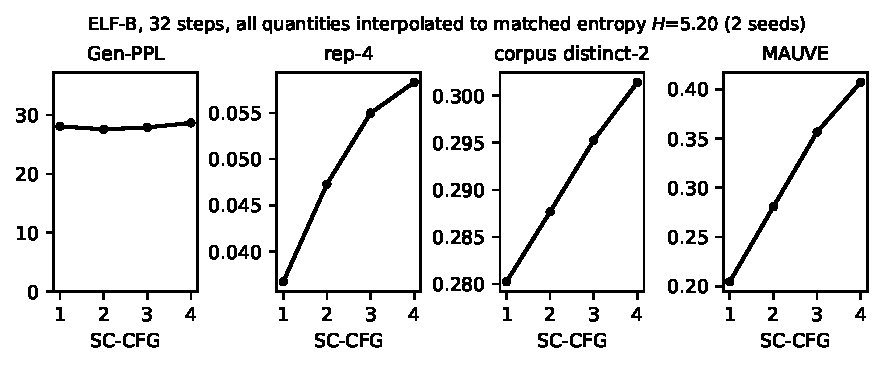
\includegraphics[width=0.72\textwidth]{paper_figures/fig_matched_entropy.pdf}
    \caption{Perplexity--entropy curves across $\text{SC-CFG} \in \{1,2,3,4\}$ on ELF-B ($K=32$, $n=2$ seeds/cell, $M=1{,}000$ samples/seed). \textbf{Left:} At matched $H_{\mathrm{ps}}=5.20$, Gen-PPL spans $1.09$ points ($27.54$--$28.63$). \textbf{Right:} Higher $\text{SC-CFG}$ with lower $\gamma$ raises \texttt{rep-4} ($0.037 \to 0.058$), corpus \texttt{distinct-2} ($0.280 \to 0.301$), and MAUVE ($0.204 \to 0.407$).}
    \label{fig:matched_entropy}
\end{figure*}

\begin{table}[ht]
    \centering
    \caption{Back-noising sweep ($\gamma \in [0, 3.0]$) on ELF-B at $\text{SC-CFG}=3.0$ ($K=32$ steps, $n=2$ seeds, $M=1{,}000$ sequences/seed), compared against OpenWebText reference subsample (\texttt{R0\_owt\_ref}).}
    \label{tab:gamma_sweep}
    \resizebox{\columnwidth}{!}{% AUTO-GENERATED by analysis/make_figures_tables.py -- do not edit
\begin{tabular}{rrrrrr}
\toprule
$\gamma$ & Gen-PPL & $H$ (nats) & rep-4 & distinct-2 & MAUVE \\
\midrule
0 & 45.66 & 5.304 & 0.050 & 0.356 & 0.624 \\
0.25 & 40.19 & 5.283 & 0.050 & 0.343 & 0.592 \\
0.5 & 35.71 & 5.260 & 0.050 & 0.329 & 0.543 \\
1 & 28.87 & 5.210 & 0.054 & 0.300 & 0.385 \\
1.5 & 24.04 & 5.156 & 0.061 & 0.273 & 0.235 \\
2 & 20.77 & 5.097 & 0.071 & 0.251 & 0.158 \\
3 & 16.70 & 4.946 & 0.108 & 0.214 & 0.081 \\
\midrule
OWT ref. & 17.18 & 5.404 & 0.030 & 0.440 & -- \\
\bottomrule
\end{tabular}
}
\end{table}

\begin{table}[ht]
    \centering
    \caption{Raw $\gamma=0$ Generative Perplexity vs.\ linear interpolations at matched per-sample entropies $H_{\mathrm{ps}} \in \{5.15, 5.20\}$ nats across $\text{SC-CFG} \in \{1, 2, 3, 4\}$ on ELF-B ($n=2$ seeds/cell, $M=1{,}000$ sequences/seed).}
    \label{tab:matched_entropy_app}
    \resizebox{\columnwidth}{!}{% AUTO-GENERATED by analysis/make_figures_tables.py -- do not edit
\begin{tabular}{lrrrr}
\toprule
SC-CFG & 1 & 2 & 3 & 4 \\
\midrule
Gen-PPL at $\gamma{=}0$ (raw) & 103.6 & 59.2 & 45.7 & 43.6 \\
\midrule \multicolumn{5}{l}{\emph{interpolated to matched entropy $H=5.15$}} \\
Gen-PPL & 24.49 & 23.85 & 23.68 & 24.05 \\
\multicolumn{5}{l}{\emph{interpolated to matched entropy $H=5.20$}} \\
Gen-PPL & 28.06 & 27.54 & 27.88 & 28.63 \\
rep-4 & 0.037 & 0.047 & 0.055 & 0.058 \\
corpus distinct-2 & 0.280 & 0.288 & 0.295 & 0.301 \\
MAUVE & 0.204 & 0.281 & 0.357 & 0.407 \\
\bottomrule
\end{tabular}
}
\end{table}

\begin{figure*}[t]
    \centering
    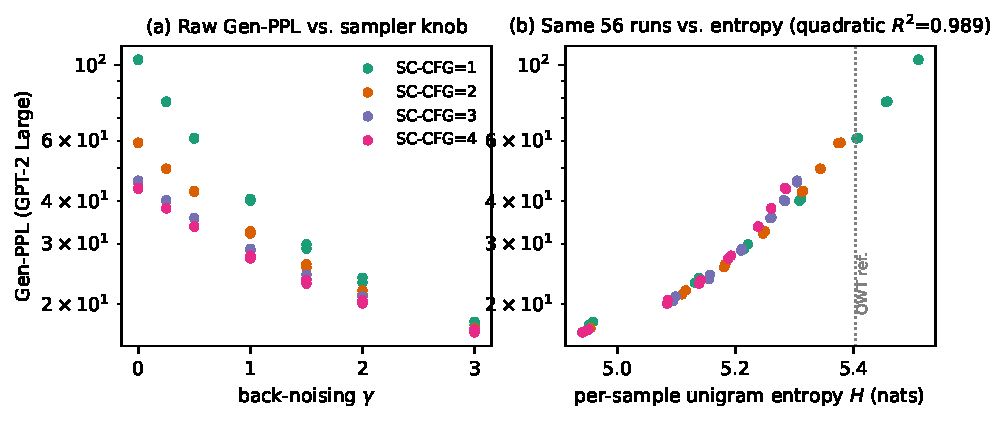
\includegraphics[width=0.92\textwidth]{paper_figures/fig_collapse.pdf}
    \caption{Uncontrolled Langevin back-noising sweep ($\gamma \in [0, 3.0]$ across $\text{SC-CFG}\in\{1,2,3,4\}$, 56 runs, $n=2$ seeds/cell, $M=1{,}000$ samples/seed) on ELF-B. \textbf{(a)} Increasing $\gamma$ drives raw Gen-PPL monotonically below the OpenWebText reference line ($17.18$; reaching $16.70$ at $\gamma=3.0, \text{SC-CFG}=3.0$), but \textbf{(b)} plotting the same 56 runs against per-sample entropy $H_{\mathrm{ps}}$ reveals that all four guidance scales collapse onto a shared trajectory (quadratic $R^2 = 0.989$) driven by entropy contraction.}
    \label{fig:collapse}
\end{figure*}

\section{Audit of Inference-Time Interventions: ECP and CMLC}
\label{app:interventions}

Table~\ref{tab:interventions} and Figure~\ref{fig:interventions} report the complete screening, 3-seed final evaluation, and control comparisons for Encoder-Conditioned Projection (ECP) and Confidence-Modulated Latent Caching (CMLC) on ELF-B (against 3-seed baseline ODE-16 Gen-PPL $98.86$ [$98.49$ in the CMLC evaluation block], 16-step SDE $\gamma=1.5$ Gen-PPL $39.23$, and global-clock fine-tune R1 ODE-16 Gen-PPL $152.01$).
Both ECP finals ($t_{\mathrm{on}}=0.50$, 3 seeds) and controls lie directly on the unmodified ELF baseline frontier ($+0.07\%$ residual at $\text{SC-CFG}=3, \gamma=1.0$ and $-0.19\%$ at $\text{SC-CFG}=1, \gamma=1.0$, $\le 0.2\%$ residual at matched entropy), while the three lower/in-range CMLC adaptive early-exit variants are strictly Pareto-dominated in the 2D $(\text{Gen-PPL}, H_{\mathrm{ps}})$ plane ($+36.3\%$, $+62.6\%$, and $+160.1\%$) and the fourth (\texttt{+ commit}, Gen-PPL $230.90$) lies above the 16-step baseline entropy range ($H_{\mathrm{ps}}=5.542$ nats).

\begin{table*}[t]
    \centering
    \caption{Evaluation of Encoder-Conditioned Projection (ECP) and Confidence-Modulated Latent Caching (CMLC) on ELF-B against matched-entropy baseline trajectories and ablation controls.}
    \label{tab:interventions}
    \resizebox{\textwidth}{!}{% AUTO-GENERATED by analysis/make_figures_tables.py -- do not edit
\begin{tabular}{lrrrrrrrl}
\toprule
Configuration & seeds & $n$ & NFE (flow/enc) & Gen-PPL & $\Delta H$ & MAUVE & baseline PPL at $H$ & entropy-adjusted change \\
\midrule
\multicolumn{9}{l}{\emph{(a) ECP screening runs, $t_{\mathrm{on}}{=}0.30$, single seed}} \\
ECP hard (SC), ODE-16 & 1 & 512 & 27/29 & 88.06 & -0.024 & 0.685 & 88.34 & -0.3\% \\
ECP soft (SC), ODE-16 & 1 & 256 & 28/15 & 84.25 & -0.028 & 0.836 & 86.84 & -3.0\% \\
ECP hard (SC), ODE-32 & 1 & 512 & 48/48 & 41.29 & -0.012 & 0.717 & 43.18 & -4.4\% \\
ECP hard (SC), $k{=}2$, ODE-32 & 1 & 512 & 42/25 & 41.59 & -0.013 & 0.722 & 43.02 & -3.3\% \\
ECP hard (SC), SDE-32 $\gamma{=}$1.5 & 1 & 512 & 48/48 & 23.85 & +0.001 & 0.314 & 24.31 & -1.9\% \\
ECP hard (z-weak), SDE-32 $\gamma{=}$1.5 & 1 & 512 & 48/48 & 23.74 & -0.006 & 0.323 & 23.91 & -0.7\% \\
\midrule
\multicolumn{9}{l}{\emph{(b) ECP finals with controls, $t_{\mathrm{on}}{=}0.50$, three seeds}} \\
ECP hard (SC), ODE-16 & 3 & 1000 & 22/12 & 98.40 & -0.001 & 0.442 & 98.46 & -0.1\% \\
ECP hard (SC), ODE-32 & 3 & 1000 & 39/24 & 45.74 & -0.001 & 0.594 & 45.70 & +0.1\% \\
ECP hard (SC+z-weak), ODE-16 & 3 & 1000 & 22/12 & 98.42 & -0.001 & 0.467 & 98.49 & -0.1\% \\
ECP hard (SC+z-weak), ODE-32 & 3 & 1000 & 39/24 & 45.75 & -0.001 & 0.596 & 45.71 & +0.1\% \\
Control A5: matched-norm random, ODE-16 & 3 & 1000 & 22/12 & 98.84 & +0.000 & 0.426 & -- & out of range \\
Control A5: matched-norm random, ODE-32 & 3 & 1000 & 39/24 & 45.91 & -0.000 & 0.610 & 45.96 & -0.1\% \\
Control A6: non-contextual re-encode, ODE-16 & 3 & 1000 & 22/12 & 98.40 & -0.001 & 0.410 & 98.36 & +0.0\% \\
Control A6: non-contextual re-encode, ODE-32 & 3 & 1000 & 39/24 & 45.75 & -0.001 & 0.494 & 45.67 & +0.2\% \\
Baseline B6: restart, ODE-16 & 3 & 1000 & 22/12 & 79.83 & -0.053 & 0.525 & 77.61 & +2.9\% \\
Baseline B6: restart, ODE-32 & 3 & 1000 & 39/24 & 40.88 & -0.025 & 0.644 & 40.40 & +1.2\% \\
\midrule
\multicolumn{9}{l}{\emph{(c) CMLC, fine-tuned R3 model, three seeds}} \\
CMLC R3 adaptive-ent (ODE-16) & 3 & 1000 & 82/0 & 92.35 & -0.634 & -- & -- & Pareto-dominated \\
CMLC R3 adaptive-stab (SDE-16, $\gamma{=}$1.0) & 3 & 1000 & 18/0 & 115.45 & -0.180 & -- & -- & Pareto-dominated \\
CMLC R3 adaptive-stab + commit (ODE-16) & 3 & 1000 & 23/0 & 230.90 & +0.061 & -- & -- & out of range \\
CMLC R3 adaptive-stab (ODE-16) & 3 & 1000 & 18/0 & 200.85 & -0.054 & -- & 77.22 & +160.1\% \\
\bottomrule
\end{tabular}
}
\end{table*}

\begin{figure*}[t]
    \centering
    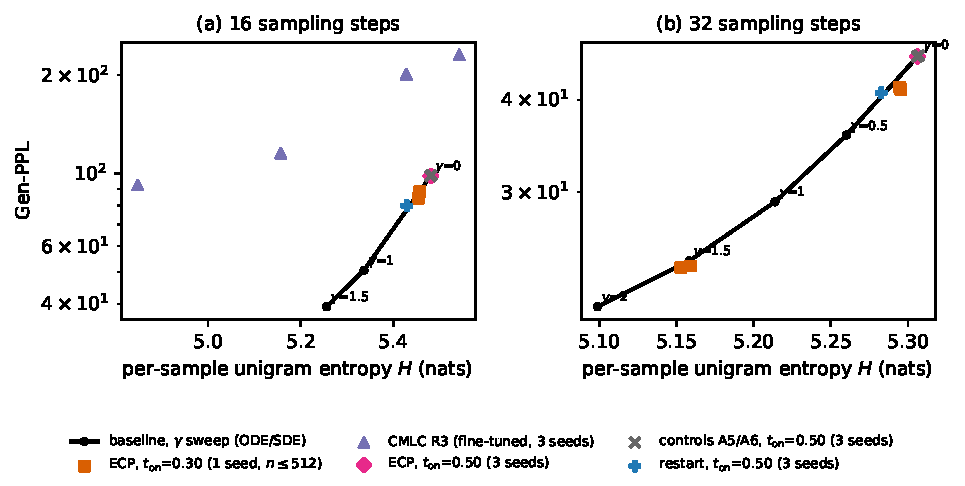
\includegraphics[width=0.92\textwidth]{paper_figures/fig_interventions.pdf}
    \caption{Trajectory interventions plotted in the $(\text{Gen-PPL}, H_{\mathrm{ps}})$ plane on ELF-B. Both ECP finals ($t_{\mathrm{on}}=0.50$, 3 seeds) and controls lie directly on the unmodified ELF baseline frontier ($\le 0.2\%$ residual at matched entropy), while the three lower/in-range CMLC adaptive early-exit variants are strictly Pareto-dominated in the 2D $(\text{Gen-PPL}, H_{\mathrm{ps}})$ plane ($+36.3\%$ to $+160.1\%$) and the fourth (\texttt{+ commit}, Gen-PPL $230.90$) lies above the 16-step baseline entropy range ($H_{\mathrm{ps}}=5.542$ nats).}
    \label{fig:interventions}
\end{figure*}

\section{Model-Scale Frontiers and Cross-Paradigm Discrete Diffusion (MDLM)}
\label{app:scale_cross}

Table~\ref{tab:elfm_m1} and Table~\ref{tab:elfl_l1} report the ELF-M (342.5M) Pair M1 evaluation and ELF-L (652.1M) Pair L1 evaluation alongside their seed-blocked $2\times 2$ factorial main effects. Table~\ref{tab:scale} reports the model-scale frontier comparison across ELF-B (104.6M, interpolated $\text{PPL}@H=5.15$ of $23.68$), ELF-M (342.5M, interpolated $\text{PPL}@H=5.15$ of $19.54$ and $\text{PPL}@H=5.20$ of $23.42$), and ELF-L (652.1M, boundary $\text{Gen-PPL}=21.59$ at $H_{\mathrm{ps}}=5.2402$; $\text{PPL}@H=5.15$ not reported as $5.15 \notin [5.240, 5.287]$). Table~\ref{tab:cross_paradigm} and Figure~\ref{fig:cross_paradigm} report the cross-paradigm step-budget comparison between continuous-latent ELF-B (reaching $N=64$ Gen-PPL of $54.82$ at $\gamma=0$, $28.53$ at $\gamma=1.0$, and $22.77$ at $\gamma=1.5$) and discrete Masked Diffusion Language Models (MDLM, 130M backbone / 170M total parameters, Gen-PPL $147.80$ at $N=64$)~\citep{sahoo2024mdlm,zheng2025masked}.

\begin{table*}[t]
    \centering
    \caption{ELF-M (342.5M backbone, $K=64$) exploratory Pair M1 evaluation and seed-blocked $2\times 2$ factorial main effects ($n=5$ complete blocks, $df=4$, $M=1{,}000$/seed; Pair M1 passes Tier-I equivalence on Gen-PPL at $p_{\mathrm{TOST,I}}=0.0052$, fails strict Tier-I on $H_{\mathrm{ps}}$ at $\Delta H_{\mathrm{ps}}=-0.0210$~nats vs.\ $\pm 0.015$~nats bound [$p_{\mathrm{TOST,I}}=0.9889$], and satisfies only the post-hoc exploratory Tier-II tolerance $\pm 0.025$~nats at $p_{\mathrm{TOST,II,paired}}=0.0354$). Full panels in Appendix~\ref{app:full_tables}, Tables~\ref{tab:elfm_m1_full}--\ref{tab:elfl_l1_full}.}
    \label{tab:elfm_m1}
    \resizebox{\textwidth}{!}{% AUTO-GENERATED by analysis/generate_revised_tables.py -- do not edit manually
\begingroup
\small
\setlength{\tabcolsep}{4.0pt}
\renewcommand{\arraystretch}{1.12}
\begin{tabular}{llcccc}
\toprule
Contrast / Condition & Metric & Arm A ($1.0, 2.00$) & Arm B ($4.0, 0.50$) & Difference $\Delta$ [95\% Paired CI] & Test Decision / $p$-value \\
\midrule
Pair M1 (ELF-M, $df{=}4$) & Gen-PPL & $23.02\pm0.20$ & $23.11\pm0.23$ & $+0.09$ $[-0.20,\,+0.39]$ & Tier-I Equiv ($p_{\mathrm{TOST}}=0.0052$) \\
 & $H_{\mathrm{ps}}$ (nats) & $5.2108\pm0.0049$ & $5.1898\pm0.0069$ & $-0.0210$ $[-0.0255,\,-0.0164]$ & Non-Equiv T-I ($p_{\mathrm{TOST,I}}=0.9889$); Expl.\ T-II ($0.0354$; $p_{\mathrm{diff}}=0.0002$) \\
 & rep-4 (\%) & $2.97\pm0.06$ & $6.44\pm0.13$ & $+3.47$ pp $[+3.38,\,+3.56]$ & $p_{\mathrm{paired}} < 0.0001$ \\
 & $\mathrm{JSD}_\pi$ (nats) & $1.6774\pm0.0119$ & $1.9548\pm0.0066$ & $+0.2774$ $[+0.2687,\,+0.2862]$ & $p_{\mathrm{paired}} < 0.0001$ \\
 & MAUVE & $0.348\pm0.038$ & $0.531\pm0.030$ & $+0.183$ $[+0.142,\,+0.224]$ & $p_{\mathrm{paired}} = 0.0002$ \\
\midrule
Factorial Main Effects & $\Delta_{\mathrm{SC}}$ ($4.0 - 1.0$) & \multicolumn{2}{c}{$n=5$ Complete Blocks ($df=4$)} & $+3.67$ pp rep-4 ($2.20\!\times\!10^{-8}$) & $+0.127$ nats $\mathrm{JSD}_\pi$ \\
 & $\Delta_\gamma$ ($2.0 - 0.5$) & \multicolumn{2}{c}{$n=5$ Complete Blocks ($df=4$)} & $+0.20$ pp rep-4 ($0.0037$) & $-0.151$ nats $\mathrm{JSD}_\pi$ \\
 & Interaction $I_s$ & \multicolumn{2}{c}{$\Delta_{\mathrm{SC}}(0.5) - \Delta_{\mathrm{SC}}(2.0)$} & $+0.82$ pp rep-4 ($5.63\!\times\!10^{-5}$) & $-0.032$ nats $\mathrm{JSD}_\pi$ \\
\midrule
\multicolumn{6}{@{}p{\linewidth}@{}}{\footnotesize Paired seed-level 95\% CIs ($\bar{d}\pm t_{0.975,4}\cdot\mathrm{SE}_{\mathrm{paired}}$, $df=4$, seeds $0\text{--}4$). Backbone parameters exclude the frozen T5-small encoder (~35.3M parameters). $K=64$, $M=1{,}000$/seed. Tier-II ($\pm 0.025$ nats $H_{\mathrm{ps}}$) is a post-hoc exploratory tolerance (not preregistered).} \\
\bottomrule
\end{tabular}
\endgroup
}
\end{table*}

\begin{table*}[t]
    \centering
    \caption{ELF-L (652.1M backbone, $6.2\times$ scale, $K=64$) Pair L1 evaluation and seed-blocked $2\times 2$ factorial main effects ($n=3$ complete blocks $df=2$; 5-seed paired contrast $df=4$). Full multi-column panel in Appendix~\ref{app:full_tables}, Table~\ref{tab:elfl_l1_full}.}
    \label{tab:elfl_l1}
    \makebox[\textwidth][c]{% AUTO-GENERATED by analysis/generate_revised_tables.py -- do not edit manually
\begingroup
\small
\setlength{\tabcolsep}{4.0pt}
\renewcommand{\arraystretch}{1.12}
\begin{tabular}{llcccc}
\toprule
Contrast / Condition & Metric & Arm A ($1.0, 2.00$) & Arm B ($4.0, 0.50$) & Difference $\Delta$ [95\% CI] & Test Decision / $p$-value \\
\midrule
Pair L1 (ELF-L, $n{=}5$ paired) & Gen-PPL & $25.84\pm0.23$ & $22.02\pm0.14$ & $-3.84$ $[-4.18,\,-3.49]$ & $6.57\!\times\!10^{-6}$ ($df{=}4$) \\
 & $H_{\mathrm{ps}}$ (nats) & $5.3058\pm0.0077$ & $5.2516\pm0.0096$ & $-0.0536$ $[-0.0664,\,-0.0408]$ & $0.0003$ ($df{=}4$) \\
 & rep-4 (\%) & $2.61\pm0.13$ & $6.94\pm0.28$ & $+4.38$ pp $[+4.01,\,+4.75]$ & $4.91\!\times\!10^{-6}$ ($df{=}4$) \\
 & $\mathrm{JSD}_\pi$ (nats) & $1.7241\pm0.0092$ & $1.8890\pm0.0115$ & $+0.1649$ $[+0.1505,\,+0.1793]^{\mathrm{a}}$ & $p_{\mathrm{Wald}} < 0.0001$ \\
 & MAUVE & $0.333\pm0.040$ & $0.352\pm0.010$ & $-0.032$ $[-0.081,\,+0.017]$ & $p_{\mathrm{paired}} = 0.145$ \\
\midrule
Factorial Main Effects & $\Delta_{\mathrm{SC}}$ ($4.0 - 1.0$) & \multicolumn{2}{c}{$n=3$ Complete Blocks ($df=2$)} & $+3.40$ pp rep-4 ($p=0.0009$) & $+0.074$ nats $\mathrm{JSD}_\pi$ \\
 & $\Delta_\gamma$ ($2.0 - 0.5$) & \multicolumn{2}{c}{$n=3$ Complete Blocks ($df=2$)} & $-1.17$ pp rep-4 ($p=0.0057$) & $-0.130$ nats $\mathrm{JSD}_\pi$ \\
 & Interaction $I_s$ & \multicolumn{2}{c}{$\Delta_{\mathrm{SC}}(0.5) - \Delta_{\mathrm{SC}}(2.0)$} & $+2.53$ pp rep-4 ($p=0.0007$) & $+0.038$ nats $\mathrm{JSD}_\pi$ \\
\midrule
\multicolumn{6}{@{}p{\linewidth}@{}}{\footnotesize Paired seed-level 95\% CIs ($\bar{d}\pm t_{0.975,4}\cdot\mathrm{SE}_{\mathrm{paired}}$, $df=4$, seeds $201\text{--}205$) for Gen-PPL, $H_{\mathrm{ps}}$, rep-4, and MAUVE; $^{\mathrm{a}}\mathrm{JSD}_\pi$ 95\% CI from the 16-run cell-means sensitivity model ($df=12$). Backbone parameters exclude the frozen T5-small encoder (~35.3M parameters). $K=64$, $M=500$/seed.} \\
\bottomrule
\end{tabular}
\endgroup
}
\end{table*}

\begin{table}[ht]
    \centering
    \caption{Model-scale comparison across ELF-B (104.6M, 32 steps), ELF-M (342.5M, 64 steps), and ELF-L (652.1M, 64 steps) along $\text{SC-CFG}=3$ $\gamma$-sweeps.}
    \label{tab:scale}
    \resizebox{\columnwidth}{!}{% AUTO-GENERATED by analysis/make_figures_tables.py -- do not edit
\begin{tabular}{lrrrr}
\toprule
Model (steps) & observed $H$ range & PPL@5.15 & PPL@5.20 & PPL@5.24 \\
\midrule
ELF-B 105M (32) & [4.946, 5.304] & 23.68 & 27.88 & 32.76 \\
ELF-M 342M (64) & [5.125, 5.236] & 19.54 & 23.42 & n/r \\
ELF-L 652M (64) & [5.240, 5.287] & n/r & n/r & n/r \\
\bottomrule
\end{tabular}
}
\end{table}

\begin{table*}[t]
    \centering
    \caption{Cross-paradigm comparison between continuous-latent ELF-B (104.6M backbone) and discrete Masked Diffusion Language Models (MDLM, 130M backbone / 170M total) across step budgets $N \in \{4, 8, 16, 32, 64\}$.}
    \label{tab:cross_paradigm}
    \resizebox{\textwidth}{!}{% AUTO-GENERATED by analysis/make_figures_tables.py -- do not edit
\begin{tabular}{rrrrrrrr}
\toprule
$N$ & ELF $\gamma$ & ELF Gen-PPL & ELF dedup-PPL & ELF rep-4 & pooled $H$ & MDLM Gen-PPL at $H$ & MDLM dedup-PPL at $H$ \\
\midrule
4 & 0 & 351.35 & 346.91 & 0.000 & 7.93 & 713.6 & 815.6 \\
4 & 1 & 11.34 & 13.49 & 0.101 & 4.31 & 23.0 & 27.2 \\
4 & 1.5 & 2.82 & 6.17 & 0.644 & 1.81 & out of range & out of range \\
8 & 0 & 181.37 & 180.79 & 0.000 & 7.86 & 292.1 & 356.3 \\
8 & 1 & 36.44 & 38.60 & 0.023 & 6.40 & 48.0 & 69.3 \\
8 & 1.5 & 2.99 & 5.30 & 0.501 & 2.13 & out of range & out of range \\
16 & 0 & 79.64 & 82.30 & 0.004 & 7.76 & 120.1 & 145.3 \\
16 & 1 & 44.59 & 47.49 & 0.008 & 7.40 & 65.5 & 84.3 \\
16 & 1.5 & 8.98 & 14.58 & 0.247 & 3.92 & 4.9 & 11.3 \\
32 & 0 & 41.93 & 49.11 & 0.022 & 7.64 & 67.2 & 80.1 \\
32 & 1 & 26.03 & 32.31 & 0.031 & 7.39 & 43.4 & 53.5 \\
32 & 1.5 & 49.91 & 59.85 & 0.032 & 7.26 & 34.5 & 43.4 \\
64 & 0 & 26.37 & 40.49 & 0.073 & 7.57 & 49.2 & 58.4 \\
64 & 1 & 18.40 & 29.79 & 0.088 & 7.40 & 36.2 & 43.8 \\
64 & 1.5 & 19.04 & 31.75 & 0.092 & 7.34 & 32.4 & 39.6 \\
\bottomrule
\end{tabular}
}
\end{table*}

\begin{figure*}[t]
    \centering
    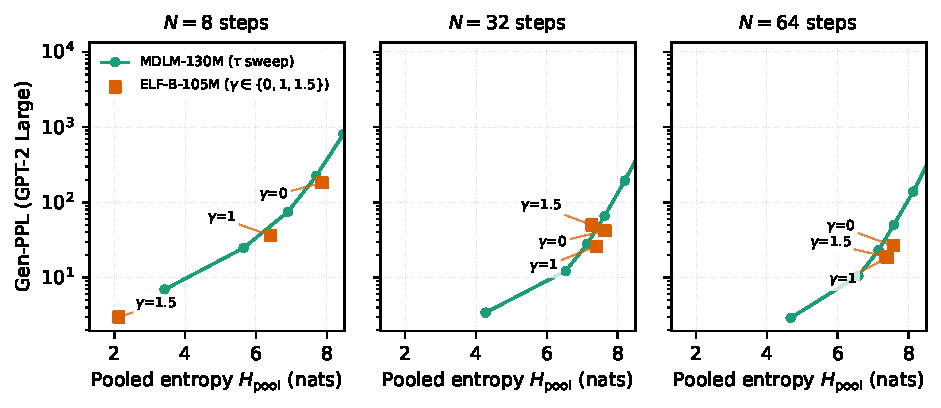
\includegraphics[width=0.92\textwidth]{paper_figures/fig_cross_paradigm.pdf}
    \caption{Cross-paradigm step-budget trajectories ($N \in \{8,32,64\}$) for ELF-B ($\gamma \in \{0, 1.0, 1.5\}$) and discrete MDLM in the $(\text{Gen-PPL}, H_{\mathrm{pool}})$ plane.}
    \label{fig:cross_paradigm}
\end{figure*}

\section{Authoritative Experimental Inventory and Reproducibility}
\label{app:inventory}

To ensure complete scientific reproducibility, all 529 baseline model generation runs, 1 OpenWebText reference run, and all confirmatory revision suites---the 120-run 20-seed C1--C3 replication (\path{runs/replication_c1_c3/}), the 13-gram decontaminated held-out reference audit (\path{runs/heldout_reference/}), the 3-judge position-swapped LLM evaluation panel (\path{runs/llm_judge_panel/}), the 32-run Plaid-1B $4\times 4$ response-surface audit (\path{runs/plaid_eval/}), and the $\gamma$-compensated matched-ACE plus 20-direction orthogonal null suite (\path{runs/p21_matched_ace/})---are cataloged with cryptographic SHA-256 manifests in \path{analysis/out/authoritative_experiment_inventory.json}, \path{analysis/out/final_consolidation_stats.json}, and their respective \path{runs/*/manifest.json} files.
All statistical analyses and LaTeX tables are deterministically generated by \path{analysis/final_consolidation_audit.py} and \path{analysis/generate_revised_tables.py} from raw JSON run artifacts. The standalone diagnostic package \path{frontier_audit/} provides zero-dependency CLI and programmatic interfaces for the $\kappa_m$ sensitivity diagnostic and TOST equivalence gates.

\section{Complete Full-Precision Confirmatory and Cross-Scale Tables}
\label{app:full_tables}

This appendix provides the full-precision, unabridged multi-column companion tables corresponding to the condensed tables in the main text.

\begin{table*}[p]
    \centering
    \caption{Full confirmatory operating-point equivalence (Panel A: all 13 columns including paired CRN 95\% CIs, unpaired Welch sensitivity intervals, Leave-One-Seed-Out ranges, and Hedges' $g$) and secondary distributional divergence (Panel B) across pairs \textbf{C1}--\textbf{C3} on ELF-B ($K=32, M=1{,}000$/seed) and exploratory pairs on ELF-M.}
    \label{tab:confirmatory_tost_full}
    % AUTO-GENERATED by analysis/generate_revised_tables.py -- do not edit manually
\begingroup
\scriptsize
\setlength{\tabcolsep}{2.2pt}
\renewcommand{\arraystretch}{1.08}
\textbf{Panel A: Primary Operating-Point Equivalence (Paired Seed-Blocked CRN Primary [$df=4$] \& Unpaired Welch Sensitivity; $n_A=n_B=5$ Seeds, $M=1{,}000$/Seed)}\\[2pt]
\resizebox{\textwidth}{!}{%
\begin{tabular}{llcccccccc}
\toprule
Pair (Seeds) & Metric & Arm A ($\text{SC}{=}1$) & Arm B ($\text{SC}{>}1$) & $\Delta$ ($\text{B}-\text{A}$) & 95\% Paired CI ($df{=}4$) & 95\% Welch CI (Sens.) & Paired $p_{\mathrm{TOST}}$ & Welch $p_{\mathrm{TOST}}$ & Joint Status \\
\midrule
\textbf{C1}: $(1.0,1.346)$ vs.\ $(2.0,1.000)$ ($201\text{--}205$) & Gen-PPL & $32.34\pm0.18$ & $32.52\pm0.23$ & $+0.18$ ($+0.56\%$) & $[-0.07,\,+0.43]$ & $[-0.12,\,+0.49]$ & $\mathbf{0.0011}$ & $0.0009$ & \textbf{Tier-I Equiv.} ($0.0011$ / $0.0021$) \\
 & $H_{\mathrm{ps}}$ (nats) & $5.2479\pm0.0051$ & $5.2489\pm0.0059$ & $+0.0010$ & $[-0.0025,\,+0.0045]$ & $[-0.0071,\,+0.0091]$ & $\mathbf{0.0002}$ & $0.0021$ & 90\% CI: $[-0.01,+0.37]$, $[-0.0017,+0.0037]$ \\
\midrule
\textbf{C2}: $(1.0,1.547)$ vs.\ $(3.0,1.000)$ ($201\text{--}205$) & Gen-PPL & $28.89\pm0.15$ & $28.92\pm0.28$ & $+0.03$ ($+0.10\%$) & $[-0.18,\,+0.24]$ & $[-0.31,\,+0.37]$ & $\mathbf{0.0004}$ & $0.0012$ & \textbf{Tier-I Equiv.} ($0.0004$ / $0.0022$) \\
 & $H_{\mathrm{ps}}$ (nats) & $5.2118\pm0.0047$ & $5.2105\pm0.0060$ & $-0.0013$ & $[-0.0046,\,+0.0020]$ & $[-0.0092,\,+0.0067]$ & $\mathbf{0.0002}$ & $0.0022$ & 90\% CI: $[-0.13,+0.19]$, $[-0.0038,+0.0013]$ \\
\midrule
\textbf{C3}: $(1.0,1.651)$ vs.\ $(4.0,1.000)$ ($201\text{--}205$) & Gen-PPL & $27.41\pm0.12$ & $27.56\pm0.27$ & $+0.15$ ($+0.54\%$) & $[-0.13,\,+0.43]$ & $[-0.18,\,+0.48]$ & $\mathbf{0.0030}$ & $0.0040$ & \textbf{Tier-I Equiv.} ($0.0030$ / $0.0126$) \\
 & $H_{\mathrm{ps}}$ (nats) & $5.1942\pm0.0043$ & $5.1897\pm0.0069$ & $-0.0045$ & $[-0.0092,\,+0.0002]$ & $[-0.0132,\,+0.0042]$ & $\mathbf{0.0018}$ & $0.0126$ & 90\% CI: $[-0.07,+0.36]$, $[-0.0081,-0.0009]$ \\
\midrule
\textbf{R1} (Expl.): $(1.0,1.250)$ vs.\ $(3.0,0.500)$ ($0\text{--}4$) & Gen-PPL & $34.37\pm0.19$ & $35.85\pm0.33$ & $+1.48$ ($+4.31\%$) & $[+0.99,\,+1.98]$ & $[+1.07,\,+1.89]$ & $0.9875$ & $0.9951$ & Non-Equiv. ($\Delta\text{PPL}{=}{+}4.31\%$) \\
 & $H_{\mathrm{ps}}$ (nats) & $5.2678\pm0.0038$ & $5.2630\pm0.0053$ & $-0.0047$ & $[-0.0127,\,+0.0033]$ & $[-0.0116,\,+0.0022]$ & $0.0118$ & $0.0047$ & ($df_{\mathrm{Satt}}=6.3,\,7.2$) \\
\midrule
\textbf{R2} (Expl.): $(1.0,1.750)$ vs.\ $(4.0,1.000)$ ($0\text{--}4$) & Gen-PPL & $26.24\pm0.32$ & $27.58\pm0.29$ & $+1.35$ ($+5.14\%$) & $[+0.99,\,+1.71]$ & $[+0.91,\,+1.79]$ & $0.9970$ & $0.9966$ & Non-Equiv. ($\Delta\text{PPL}{=}{+}5.14\%$) \\
 & $H_{\mathrm{ps}}$ (nats) & $5.1798\pm0.0023$ & $5.1922\pm0.0033$ & $+0.0123$ & $[+0.0068,\,+0.0178]$ & $[+0.0081,\,+0.0166]$ & $0.1249$ & $0.0924$ & ($df_{\mathrm{Satt}}=7.9,\,7.2$) \\
\midrule
\textbf{S1} (Expl.): $(1.0,2.000)$ vs.\ $(4.0,1.500)$ ($0\text{--}4$) & Gen-PPL & $23.49\pm0.36$ & $23.27\pm0.22$ & $-0.23$ ($-0.96\%$) & $[-0.49,\,+0.04]$ & $[-0.68,\,+0.23]$ & $0.0095$ & $0.0501$ & Expl.\ Tier-II ($0.0009$; Paired T-I $0.0095$)$^{\dagger}$ \\
 & $H_{\mathrm{ps}}$ (nats) & $5.1355\pm0.0032$ & $5.1399\pm0.0022$ & $+0.0044$ & $[-0.0004,\,+0.0093]$ & $[+0.0003,\,+0.0085]$ & $0.0019$ & $0.0003$ & ($df_{\mathrm{Satt}}=6.6,\,7.0$) \\
\midrule
\textbf{M1} (ELF-M, Expl.): $(1.0,2.000)$ vs.\ $(4.0,0.500)$ ($0\text{--}4$) & Gen-PPL & $23.02\pm0.20$ & $23.11\pm0.23$ & $+0.09$ ($+0.41\%$) & $[-0.20,\,+0.39]$ & $[-0.22,\,+0.41]$ & $0.0052$ & $0.0040$ & PPL T-I ($0.0052$); $H_{\mathrm{ps}}$ Non-Eq T-I ($0.9889$), T-II ($0.0354$)$^{\ddagger}$ \\
 & $H_{\mathrm{ps}}$ (nats) & $5.2108\pm0.0049$ & $5.1898\pm0.0069$ & $-0.0210$ & $[-0.0255,\,-0.0164]$ & $[-0.0299,\,-0.0120]$ & $0.9889$ & $0.9207$ & ($df_{\mathrm{Satt}}=7.8,\,7.2$) \\
\bottomrule
\end{tabular}%
}\par\vspace{2pt}
{\footnotesize\noindent \emph{Minimum passing margins} $\delta_{\min}{=}|\Delta|{+}t_{0.95,df}\mathrm{SE}_{\Delta}$ (C1, C2, C3): Gen-PPL $\pm 0.427$ ($\pm 1.32\%$), $\pm 0.278$ ($\pm 0.96\%$), $\pm 0.410$ ($\pm 1.50\%$); $H_{\mathrm{ps}}$ $\pm 0.0076$, $\pm 0.0079$, $\pm 0.0114$ nats. Tier-I ($\pm 2.5\%$ PPL, $\pm 0.015$ nats $H_{\mathrm{ps}}$) is the preregistered primary equivalence bound; Tier-II ($\pm 5.0\%$ PPL, $\pm 0.025$ nats $H_{\mathrm{ps}}$) is a post-hoc exploratory frontier tolerance (not preregistered). All 30 confirmatory C1--C3 runs (Seeds $201\text{--}205$) and 35 local 5-seed runs (R1, R2, S1, M1; Seeds $0\text{--}4$) are verified from per-seed \texttt{summary.json} and \texttt{extended\_metrics.json} artifacts.\par}\vspace{5pt}
\textbf{Panel B: Secondary Distributional Divergence on Confirmatory Joint Tier-I Equivalent Pairs (C1, C2, C3; $n_A=n_B=5$ Seeds, $M=1{,}000$/Seed)}\\[2pt]
\resizebox{\textwidth}{!}{%
\begin{tabular}{llcccccccc}
\toprule
Confirmatory Pair & Secondary Metric & Arm A ($\text{SC}{=}1.0$) & Arm B ($\text{SC}{>}1.0$) & $\Delta$ ($\text{B}-\text{A}$) & 95\% Paired CI ($df{=}4$) & 95\% Welch CI (Sens.) & $p_{\mathrm{Holm,8,paired}}$ & $p_{\mathrm{Holm,24,paired}}$ (Welch Sens.) & Hedges' $g$ [95\% CI] \\
\midrule
\textbf{C1}: $(1.0,1.346)$ vs.\ $(2.0,1.000)$ & Within-sample rep-4 & $0.0445$ & $0.0555$ & $+0.0110$ & $[+0.0105,\,+0.0115]$ & $[+0.0104,\,+0.0116]$ & $2.78\!\times\!10^{-6}$ & $6.05\!\times\!10^{-6}$ ($1.03\!\times\!10^{-6}$) & $+25.14$ ($[+10.6,\,+39.7]$) \\
 & Within-sample distinct-2 & $0.7798$ & $0.7667$ & $-0.0131$ & $[-0.0144,\,-0.0118]$ & $[-0.0144,\,-0.0118]$ & $3.67\!\times\!10^{-5}$ & $9.18\!\times\!10^{-5}$ ($8.30\!\times\!10^{-6}$) & $-14.12$ ($[-22.4,\,-5.9]$) \\
 & Pooled entropy $H_{\mathrm{pool}}$ (nats) & $6.9760$ & $7.0479$ & $+0.0719$ & $[+0.0684,\,+0.0754]$ & $[+0.0494,\,+0.0943]$ & $3.37\!\times\!10^{-6}$ & $7.86\!\times\!10^{-6}$ ($0.0004$) & $+4.37$ ($[+1.5,\,+7.2]$) \\
 & Inter-sample $\mathrm{JSD}_\pi$ (nats) & $1.7299$ & $1.8007$ & $+0.0708$ & $[+0.0689,\,+0.0727]$ & $[+0.0535,\,+0.0881]$ & $4.23\!\times\!10^{-7}$ & $1.13\!\times\!10^{-6}$ ($0.0001$) & $+5.62$ ($[+2.1,\,+9.1]$) \\
 & Corpus distinct-2 & $0.2818$ & $0.2938$ & $+0.0120$ & $[+0.0111,\,+0.0129]$ & $[+0.0092,\,+0.0149]$ & $1.76\!\times\!10^{-5}$ & $4.23\!\times\!10^{-5}$ ($0.0001$) & $+5.71$ ($[+2.2,\,+9.3]$) \\
 & Self-BLEU-4 (\%) & $43.88$ & $41.10$ & $-2.78$ & $[-3.12,\,-2.45]$ & $[-3.62,\,-1.95]$ & $6.47\!\times\!10^{-5}$ & $0.0002$ ($0.0004$) & $-4.57$ ($[-7.5,\,-1.6]$) \\
 & CTW JCD (bpb) & $0.0982$ & $0.0872$ & $-0.0110$ & $[-0.0136,\,-0.0084]$ & $[-0.0153,\,-0.0068]$ & $0.0006$ & $0.0016$ ($0.0007$) & $-3.49$ ($[-5.9,\,-1.1]$) \\
 & MAUVE ($M{=}1{,}000$) & $0.165$ & $0.256$ & $+0.091$ & $[+0.039,\,+0.143]$ & $[+0.039,\,+0.143]$ & $0.0084$ & $0.0084^{\S}$ ($0.0040$) & $+2.39$ ($[+0.5,\,+4.3]$) \\
\midrule
\textbf{C2}: $(1.0,1.547)$ vs.\ $(3.0,1.000)$ & Within-sample rep-4 & $0.0398$ & $0.0584$ & $+0.0186$ & $[+0.0180,\,+0.0192]$ & $[+0.0178,\,+0.0193]$ & $7.27\!\times\!10^{-7}$ & $2.76\!\times\!10^{-6}$ ($5.96\!\times\!10^{-7}$) & $+34.28$ ($[+14.5,\,+54.1]$) \\
 & Within-sample distinct-2 & $0.7858$ & $0.7649$ & $-0.0209$ & $[-0.0223,\,-0.0195]$ & $[-0.0224,\,-0.0195]$ & $7.36\!\times\!10^{-6}$ & $2.39\!\times\!10^{-5}$ ($7.20\!\times\!10^{-7}$) & $-19.57$ ($[-30.9,\,-8.2]$) \\
 & Pooled entropy $H_{\mathrm{pool}}$ (nats) & $6.9248$ & $7.0362$ & $+0.1114$ & $[+0.1098,\,+0.1130]$ & $[+0.0881,\,+0.1346]$ & $3.42\!\times\!10^{-8}$ & $1.03\!\times\!10^{-7}$ ($5.29\!\times\!10^{-5}$) & $+6.56$ ($[+2.6,\,+10.6]$) \\
 & Inter-sample $\mathrm{JSD}_\pi$ (nats) & $1.7145$ & $1.8271$ & $+0.1126$ & $[+0.1105,\,+0.1147]$ & $[+0.0939,\,+0.1312]$ & $9.09\!\times\!10^{-8}$ & $2.99\!\times\!10^{-7}$ ($1.26\!\times\!10^{-5}$) & $+8.25$ ($[+3.3,\,+13.2]$) \\
 & Corpus distinct-2 & $0.2772$ & $0.2938$ & $+0.0166$ & $[+0.0162,\,+0.0170]$ & $[+0.0135,\,+0.0197]$ & $3.09\!\times\!10^{-7}$ & $1.13\!\times\!10^{-6}$ ($2.69\!\times\!10^{-5}$) & $+7.29$ ($[+2.9,\,+11.7]$) \\
 & Self-BLEU-4 (\%) & $44.32$ & $40.43$ & $-3.89$ & $[-4.54,\,-3.23]$ & $[-4.79,\,-2.98]$ & $0.0002$ & $0.0006$ ($0.0003$) & $-5.87$ ($[-9.5,\,-2.2]$) \\
 & CTW JCD (bpb) & $0.1054$ & $0.0872$ & $-0.0182$ & $[-0.0224,\,-0.0140]$ & $[-0.0232,\,-0.0132]$ & $0.0005$ & $0.0016$ ($0.0003$) & $-4.95$ ($[-8.1,\,-1.8]$) \\
 & MAUVE ($M{=}1{,}000$) & $0.203$ & $0.349$ & $+0.146$ & $[+0.092,\,+0.200]$ & $[+0.104,\,+0.188]$ & $0.0016$ & $0.0049$ ($0.0007$) & $+4.77$ ($[+1.7,\,+7.8]$) \\
\midrule
\textbf{C3}: $(1.0,1.651)$ vs.\ $(4.0,1.000)$ & Within-sample rep-4 & $0.0383\pm0.0005$ & $0.0593\pm0.0002$ & $+0.0210$ & $[+0.0203,\,+0.0217]$ & $[+0.0204,\,+0.0217]$ & $8.52\!\times\!10^{-7}$ & $2.13\!\times\!10^{-6}$ ($6.30\!\times\!10^{-8}$) & $+49.98$ ($[+21.1,\,+78.8]$) \\
 & Within-sample distinct-2 & $0.7873$ & $0.7643$ & $-0.0230$ & $[-0.0251,\,-0.0209]$ & $[-0.0252,\,-0.0209]$ & $2.75\!\times\!10^{-5}$ & $7.57\!\times\!10^{-5}$ ($3.77\!\times\!10^{-5}$) & $-14.60$ ($[-23.1,\,-6.1]$) \\
 & Pooled entropy $H_{\mathrm{pool}}$ (nats) & $6.9066$ & $7.0318$ & $+0.1252$ & $[+0.1197,\,+0.1307]$ & $[+0.1022,\,+0.1481]$ & $1.89\!\times\!10^{-6}$ & $6.05\!\times\!10^{-6}$ ($2.52\!\times\!10^{-5}$) & $+7.45$ ($[+3.0,\,+11.9]$) \\
 & Inter-sample $\mathrm{JSD}_\pi$ (nats) & $1.7024\pm0.0126$ & $1.8320\pm0.0116$ & $+0.1296$ & $[+0.1245,\,+0.1347]$ & $[+0.1119,\,+0.1473]$ & $1.61\!\times\!10^{-6}$ & $4.15\!\times\!10^{-6}$ ($3.22\!\times\!10^{-6}$) & $+10.00$ ($[+4.1,\,+15.9]$) \\
 & Corpus distinct-2 & $0.2751$ & $0.2938$ & $+0.0187$ & $[+0.0180,\,+0.0194]$ & $[+0.0154,\,+0.0219]$ & $1.61\!\times\!10^{-6}$ & $4.15\!\times\!10^{-6}$ ($1.94\!\times\!10^{-5}$) & $+7.63$ ($[+3.0,\,+12.2]$) \\
 & Self-BLEU-4 (\%) & $44.49\pm0.72$ & $40.44\pm0.40$ & $-4.05$ & $[-4.78,\,-3.32]$ & $[-4.94,\,-3.16]$ & $0.0003$ & $0.0007$ ($0.0002$) & $-6.22$ ($[-10.0,\,-2.4]$) \\
 & CTW JCD (bpb) & $0.1099$ & $0.0872$ & $-0.0227$ & $[-0.0283,\,-0.0171]$ & $[-0.0285,\,-0.0168]$ & $0.0007$ & $0.0016$ ($0.0003$) & $-5.40$ ($[-8.8,\,-2.0]$) \\
 & MAUVE ($M{=}1{,}000$) & $0.228\pm0.029$ & $0.349\pm0.029$ & $+0.121$ & $[+0.074,\,+0.168]$ & $[+0.079,\,+0.163]$ & $0.0020$ & $0.0049$ ($0.0007$) & $+3.93$ ($[+1.3,\,+6.5]$) \\
\bottomrule
\end{tabular}%
}\par\vspace{2pt}
{\footnotesize\noindent \emph{Global Holm multiplicity across all $3\times 8 = 24$ secondary pilot comparisons (seeds 201--205, not preregistered)}: \textbf{24/24} significant at $\alpha=0.05$ after global 24-way step-down Holm correction under both paired CRN tests ($df=4$, $p_{\mathrm{Holm,24,paired}} \le 0.0084 < 0.05$) and unpaired Welch sensitivity tests ($p_{\mathrm{Holm,24}} \le 0.0040$), where $^{\S}$\textbf{C1 MAUVE} has the largest paired $p$-value ($p_{\mathrm{raw,paired}}=0.0084$, rank $24/24 \implies p_{\mathrm{Holm,Fam2}}=p_{\mathrm{Holm,8,paired}}=p_{\mathrm{Holm,24,paired}}=0.0084$, passing $\alpha=0.05$ while exceeding $\alpha=0.005$; an earlier $0.0587 = 7\times 0.0084$ figure arose only when improperly pooling the 6 primary Gen-PPL/$H_{\mathrm{ps}}$ null-equivalence tests into a 30-test difference family). In the 20-seed replication (seeds 401--420), C1 MAUVE achieves $p_{\mathrm{Holm}}=5.13\!\times\!10^{-12}$. Backbone parameters exclude the frozen T5-small encoder (~35.3M parameters).\par}
\endgroup

\end{table*}

\begin{table*}[p]
    \centering
    \caption{Full ELF-M (342.5M, $K=64$) factorial results across 11 cells (29 runs, $M=1{,}000$/seed) and complete seed-blocked ANOVA contrasts ($df=4$).}
    \label{tab:elfm_m1_full}
    % AUTO-GENERATED by analysis/generate_revised_tables.py -- do not edit manually
\begingroup
\scriptsize
\setlength{\tabcolsep}{3.6pt}
\renewcommand{\arraystretch}{1.10}
\resizebox{\textwidth}{!}{%
\begin{tabular}{ccccccccc}
\toprule
SC-CFG & $\gamma$ & $n$ & Gen-PPL & $H_{\mathrm{ps}}$ & $H_{\mathrm{pool}}$ & $\mathrm{JSD}_\pi$ & rep-4 (\%) & Self-BLEU / MAUVE \\
\midrule
1.0 & 0.50 & 5 & $44.24\pm0.29$ & $5.369\pm0.004$ & $7.198\pm0.008$ & $1.829\pm0.005$ & $2.36\pm0.06$ & $29.66\pm0.41$ / $0.694\pm0.036$ \\
1.0 & 1.50 & 2 & $26.15\pm0.24$ & $5.249\pm0.007$ & $6.970\pm0.001$ & $1.721\pm0.005$ & $2.83\pm0.00$ & $35.09\pm0.07$ / $0.453\pm0.005$ \\
1.0 & 2.00 & 5 & $23.02\pm0.20$ & $5.211\pm0.005$ & $6.887\pm0.011$ & $1.677\pm0.007$ & $2.97\pm0.07$ & $39.05\pm0.40$ / $0.348\pm0.032$ \\
\midrule
3.0 & 0.00 & 1 & $39.42$ & $5.236$ & $7.163$ & $1.928$ & $6.09$ & $31.34$ / $0.586$ \\
3.0 & 0.30 & 1 & $29.74$ & $5.218$ & $7.143$ & $1.926$ & $5.41$ & $31.89$ / $0.606$ \\
3.0 & 0.50 & 1 & $26.86$ & $5.212$ & $7.119$ & $1.908$ & $5.46$ & $33.03$ / $0.618$ \\
3.0 & 1.00 & 1 & $21.97$ & $5.182$ & $7.053$ & $1.872$ & $5.36$ & $34.15$ / $0.562$ \\
3.0 & 2.00 & 1 & $17.85$ & $5.125$ & $6.906$ & $1.783$ & $5.69$ & $37.65$ / $0.273$ \\
\midrule
4.0 & 0.50 & 5 & $23.11\pm0.23$ & $5.190\pm0.007$ & $7.143\pm0.013$ & $1.955\pm0.007$ & $6.44\pm0.12$ & $32.63\pm0.41$ / $0.531\pm0.033$ \\
4.0 & 1.00 & 2 & $19.99\pm0.42$ & $5.158\pm0.008$ & $7.046\pm0.026$ & $1.889\pm0.019$ & $6.27\pm0.19$ & $34.91\pm0.57$ / $0.453\pm0.038$ \\
4.0 & 2.00 & 5 & $17.36\pm0.35$ & $5.112\pm0.008$ & $6.901\pm0.021$ & $1.790\pm0.013$ & $6.23\pm0.10$ & $37.92\pm0.55$ / $0.303\pm0.033$ \\
\midrule
\multicolumn{9}{l}{\textbf{Seed-Blocked $2\times 2$ Factorial Contrasts Across Shared Seeds $0\text{--}4$ ($n=5$ Complete Blocks, $df=4$):}} \\
\multicolumn{2}{l}{$\Delta_{\mathrm{SC}}$ ($\text{SC}{=}4.0 - 1.0$)} & 5 & $-13.39\pm0.04$ ($4.82\!\times\!10^{-10}$) & $-0.139\pm0.001$ ($1.34\!\times\!10^{-8}$) & $-0.013\pm0.002$ & $+0.127\pm0.001$ ($1.88\!\times\!10^{-8}$) & $+3.67\pm0.03$ ($2.20\!\times\!10^{-8}$) & $+0.92\pm0.05$ / $-0.104\pm0.007$ \\
\multicolumn{2}{l}{$\Delta_\gamma$ ($\gamma{=}2.0 - 0.5$)} & 5 & $-13.49\pm0.14$ ($6.44\!\times\!10^{-8}$) & $-0.118\pm0.002$ ($6.58\!\times\!10^{-7}$) & $-0.277\pm0.005$ & $-0.151\pm0.003$ ($9.17\!\times\!10^{-7}$) & $+0.20\pm0.03$ ($0.0037$) & $+7.33\pm0.09$ / $-0.287\pm0.016$ \\
\multicolumn{2}{l}{Interaction $I_s = \Delta_{\mathrm{SC}}(0.5)-\Delta_{\mathrm{SC}}(2.0)$} & 5 & $-15.46\pm0.07$ ($3.23\!\times\!10^{-9}$) & $-0.081\pm0.002$ ($4.71\!\times\!10^{-6}$) & $-0.068\pm0.004$ & $-0.032\pm0.002$ ($0.0002$) & $+0.82\pm0.05$ ($5.63\!\times\!10^{-5}$) & $+4.25\pm0.14$ / $-0.117\pm0.039$ ($0.0387$) \\
\multicolumn{2}{l}{Off-diag M1 $(4.0,0.5)-(1.0,2.0)$} & 5 & $+0.09\pm0.11$ ($0.425$) & $-0.021\pm0.002$ ($0.0002$) & $+0.256\pm0.005$ & $+0.277\pm0.003$ ($1.00\!\times\!10^{-7}$) & $+3.47\pm0.03$ ($3.86\!\times\!10^{-8}$) & $-6.42\pm0.13$ / $+0.183\pm0.015$ \\
\bottomrule
\end{tabular}%
}\\[2pt]
{\footnotesize\noindent Backbone parameters exclude the frozen T5-small encoder (~35.3M parameters). $n=5$ complete blocks (seeds $0\text{--}4$, $df=4$, $M=1{,}000$/seed). Pair M1 fails strict Tier-I equivalence on $H_{\mathrm{ps}}$ ($p_{\mathrm{TOST,I}}=0.9889$) and passes only post-hoc exploratory Tier-II ($\pm 0.025$ nats, $p_{\mathrm{TOST,II,paired}}=0.0354$).\par}
\endgroup

\end{table*}

\begin{table*}[p]
    \centering
    \caption{Full multi-seed $2\times 2$ factorial on \textbf{ELF-L (652.1M backbone)} ($K=64$, $M=500$/seed across seeds $201\text{--}205$) and cross-scale $2\times 2$ seed-blocked contrasts across ELF-B, ELF-M, and ELF-L.}
    \label{tab:elfl_l1_full}
    % AUTO-GENERATED by analysis/generate_revised_tables.py -- do not edit manually
\begingroup
\scriptsize
\setlength{\tabcolsep}{3.0pt}
\renewcommand{\arraystretch}{1.10}
\textbf{Panel A: ELF-L (652.1M [652M nominal], $d=1280$, $L=32$) $2\times 2$ Factorial Cell Balance and Summaries ($K=64$ Steps, $\mathrm{NFE}_{\mathrm{sample}}=65$, $M=500$/Seed)}\\[2pt]
\resizebox{\textwidth}{!}{%
\begin{tabular}{ccccccccccccc}
\toprule
SC-CFG & $\gamma$ & Runs ($n$) & Seeds & $M$/seed & Gen-PPL & $H_{\mathrm{ps}}$ (nats) & $H_{\mathrm{pool}}$ (nats) & $\mathrm{JSD}_\pi$ (nats) & rep-4 (\%) & within-dist-2 & distinct-2 & Self-BLEU / MAUVE \\
\midrule
1.0 & 0.50 & 3 & 201--203 & 500 & $39.70\pm0.35$ & $5.416\pm0.001$ & $7.236\pm0.001$ & $1.820\pm0.000$ & $2.49\pm0.06$ & $0.822\pm0.002$ & $0.381\pm0.002$ & $31.14\pm0.53$ / $0.483\pm0.051$ \\
1.0 & 2.00 & 5 & 201--205 & 500 & $25.84\pm0.23$ & $5.306\pm0.008$ & $7.029\pm0.016$ & $1.724\pm0.009$ & $2.61\pm0.13$ & $0.820\pm0.002$ & $0.376\pm0.002$ & $35.76\pm0.43$ / $0.333\pm0.040$ \\
4.0 & 0.50 & 5 & 201--205 & 500 & $22.02\pm0.14$ & $5.252\pm0.010$ & $7.140\pm0.021$ & $1.889\pm0.011$ & $6.94\pm0.28$ & $0.759\pm0.004$ & $0.375\pm0.002$ & $34.63\pm0.57$ / $0.352\pm0.010$ \\
4.0 & 2.00 & 3 & 201--203 & 500 & $20.59\pm0.44$ & $5.236\pm0.013$ & $7.037\pm0.023$ & $1.801\pm0.010$ & $4.69\pm0.21$ & $0.785\pm0.003$ & $0.369\pm0.002$ & $36.18\pm0.62$ / $0.230\pm0.013$ \\
\bottomrule
\end{tabular}%
}\\[2pt]
{\footnotesize\noindent\emph{Stage-1 ELF-L Baseline Sweep (Excluded from $2\times 2$ Factorial)}: $4$ local runs at $\text{SC-CFG}=3.0$, $\gamma\in\{0.0,1.0,2.0\}$ ($\text{seed}=0$, $K=64$, $M=1{,}000$; reported in Table~\ref{tab:scale}).\par}\vspace{4pt}
\textbf{Panel B: Cross-Scale $2\times 2$ ($\{\text{SC}{=}1.0,4.0\}\times\{\gamma{=}0.5,2.0\}$) Seed-Blocked Contrasts, Unbalanced Cell-Means Sensitivity, and Scale-Interaction Tests}\\[2pt]
\setlength{\tabcolsep}{2.0pt}
\resizebox{\textwidth}{!}{%
\begin{tabular}{llcccccccc}
\toprule
Model Scale ($df$) & Contrast & $\Delta\text{rep-4}$ (pp) & $\Delta\mathrm{JSD}_\pi$ & $\Delta\text{Gen-PPL}$ & $\Delta H_{\mathrm{ps}}$ & $\Delta\text{w-dist-2}$ & $\Delta\text{dist-2}$ & $\Delta\text{Self-BLEU}$ & $\Delta\text{MAUVE}$ \\
\midrule
ELF-B (105M, $4{\times}6$ desc.) & $\Delta_{\mathrm{SC}}$ ($4{-}1$) & $+3.48$ & ---$^{\mathrm{a}}$ & $-24.93$ & $-0.140$ & ---$^{\mathrm{a}}$ & $-0.036$ & ---$^{\mathrm{a}}$ & $+0.025$ \\
ELF-B (105M, $df{=}1$ desc.) & $\Delta_{\mathrm{SC}}$ ($4{-}1$) & $+3.29\pm0.07$ & ---$^{\mathrm{a}}$ & $-15.29\pm0.18$ & $-0.109\pm0.002$ & ---$^{\mathrm{a}}$ & $-0.029\pm0.000$ & ---$^{\mathrm{a}}$ & $-0.016\pm0.010$ \\
ELF-B (105M, $df{=}1$ desc.) & $\Delta_\gamma$ ($2{-}0.5$) & $+2.52\pm0.08$ & ---$^{\mathrm{a}}$ & $-25.50\pm0.26$ & $-0.213\pm0.002$ & ---$^{\mathrm{a}}$ & $-0.095$ & ---$^{\mathrm{a}}$ & $-0.340\pm0.044$ \\
ELF-B (105M, $df{=}1$ desc.) & Interaction $I_s$ & $+0.86\pm0.05$ & ---$^{\mathrm{a}}$ & $-24.19\pm0.04$ & $-0.118\pm0.002$ & ---$^{\mathrm{a}}$ & $-0.044$ & ---$^{\mathrm{a}}$ & $-0.018\pm0.004$ \\
ELF-B (105M, $df{=}1$ desc.) & Off-diag B1 & $+0.76\pm0.14$ & $+0.193\pm0.002$ & $+10.22\pm0.44$ & $+0.104\pm0.004$ & $+0.016$ & $+0.066$ & $-9.45$ & $+0.325\pm0.034$ \\
\midrule
ELF-M (342M, $df{=}4$) & $\Delta_{\mathrm{SC}}$ ($4{-}1$) & $+3.67\pm0.03$ ($2.20\!\times\!10^{-8}$) & $+0.127\pm0.001$ ($1.88\!\times\!10^{-8}$) & $-13.39\pm0.04$ ($4.82\!\times\!10^{-10}$) & $-0.139\pm0.001$ ($1.34\!\times\!10^{-8}$) & $-0.071\pm0.000$ & $-0.030\pm0.000$ & $+0.92\pm0.05$ & $-0.104\pm0.007$ ($0.0001$) \\
ELF-M (342M, $df{=}4$) & $\Delta_\gamma$ ($2{-}0.5$) & $+0.20\pm0.03$ ($0.0037$) & $-0.151\pm0.003$ ($9.17\!\times\!10^{-7}$) & $-13.49\pm0.14$ ($6.44\!\times\!10^{-8}$) & $-0.118\pm0.002$ ($6.58\!\times\!10^{-7}$) & $-0.027$ & $-0.065$ & $+7.33$ & $-0.287\pm0.016$ ($5.40\!\times\!10^{-5}$) \\
ELF-M (342M, $df{=}4$) & Interaction $I_s$ & $+0.82\pm0.05$ ($5.63\!\times\!10^{-5}$) & $-0.032\pm0.002$ ($0.0002$) & $-15.46\pm0.07$ ($3.23\!\times\!10^{-9}$) & $-0.081\pm0.002$ ($4.71\!\times\!10^{-6}$) & $-0.026$ ($1.36\!\times\!10^{-6}$) & $-0.039$ ($3.98\!\times\!10^{-7}$) & $+4.25$ ($7.76\!\times\!10^{-6}$) & $-0.117\pm0.039$ ($0.0387$) \\
ELF-M (342M, M1 $df{=}4$) & Off-diag M1 & $+3.47\pm0.03$ ($3.86\!\times\!10^{-8}$) & $+0.277\pm0.003$ ($1.00\!\times\!10^{-7}$) & $+0.09\pm0.11$ ($0.425$) & $-0.021\pm0.002$ ($0.0002$) & $-0.044$ & $+0.035$ & $-6.42$ & $+0.183\pm0.015$ ($0.0002$) \\
\midrule
ELF-L (652M, $df{=}2$ pri.) & $\Delta_{\mathrm{SC}}$ ($4{-}1$) & $+3.40\pm0.10$ ($0.0009$) & $+0.074\pm0.004^{\mathrm{c}}$ & $-11.50\pm0.28$ ($0.0006$) & $-0.120\pm0.007$ ($0.0031$) & $-0.049\pm0.002^{\mathrm{c}}$ & $-0.007\pm0.001^{\mathrm{c}}$ & $+1.97\pm0.35^{\mathrm{c}}$ & $-0.133\pm0.025$ ($0.0348$) \\
ELF-L (652M, $df{=}12$ sens.) & $\Delta_{\mathrm{SC}}$ ($4{-}1$) & $+3.26\pm0.09$ & $+0.073\pm0.004$ & $-11.47\pm0.17$ & $-0.117\pm0.005$ & $-0.049\pm0.001$ & $-0.007\pm0.001$ & $+1.96\pm0.28$ & $-0.117\pm0.018$ \\
ELF-L (652M, $df{=}2$ pri.) & $\Delta_\gamma$ ($2{-}0.5$) & $-1.17\pm0.09$ ($0.0057$) & $-0.092\pm0.004^{\mathrm{c}}$ & $-7.60\pm0.15$ ($0.0004$) & $-0.061\pm0.001$ ($0.0003$) & $+0.012^{\mathrm{c}}$ & $-0.006^{\mathrm{c}}$ & $+3.08^{\mathrm{c}}$ & $-0.119\pm0.016$ ($0.0185$) \\
ELF-L (652M, $df{=}2$ pri.) & Interaction $I_s$ & $+2.53\pm0.07$ ($0.0007$) & $-0.008\pm0.009^{\mathrm{c}}$ ($p=0.385$) & $-12.55\pm0.43$ ($0.0012$) & $-0.103\pm0.008$ ($0.0055$) & $-0.028^{\mathrm{c}}$ & $+0.001^{\mathrm{c}}$ & $+3.07^{\mathrm{c}}$ & $+0.001\pm0.020$ ($0.977$) \\
ELF-L (652M, L1 $df{=}4$)$^{\mathrm{b}}$ & Off-diag L1 ($n{=}5$) & $+4.38\pm0.13$ ($4.91\!\times\!10^{-6}$) & $+0.165\pm0.007^{\mathrm{c}}$ & $-3.84\pm0.12$ ($6.57\!\times\!10^{-6}$) & $-0.054\pm0.005$ ($0.0003$) & $-0.061^{\mathrm{c}}$ & $-0.001^{\mathrm{c}}$ & $-1.13^{\mathrm{c}}$ & $-0.032\pm0.018$ ($0.145$)$^{\mathrm{d}}$ \\
ELF-L (652M, L1 $df{=}2$)$^{\mathrm{b}}$ & Off-diag L1 ($n{=}3$) & $+4.57\pm0.12$ ($0.0007$) & ---$^{\mathrm{c}}$ & $-3.90\pm0.21$ ($0.0029$) & $-0.059\pm0.006$ ($0.0092$) & ---$^{\mathrm{c}}$ & ---$^{\mathrm{c}}$ & ---$^{\mathrm{c}}$ & $-0.014\pm0.023$ ($0.618$) \\
\midrule
Scale Int.\ (ELF-L $-$ ELF-M) & Welch ($df_{\mathrm{Satt}}\in[2.1,2.3]$) & $-0.27\pm0.10$ ($0.1022$) & $-0.053\pm0.006^{\mathrm{c}}$ & $+1.89\pm0.29$ ($0.0202$) & $+0.020\pm0.007$ ($0.0953$) & $+0.022\pm0.002^{\mathrm{c}}$ & \emph{Unmatched $M$} & \emph{Unmatched $M$} & \emph{Unmatched $M$} \\
Scale Int.\ (ELF-M $-$ ELF-B) & Descriptive ($n_B{=}2$) & $+0.39\pm0.07$ (desc.) & ---$^{\mathrm{a}}$ & $+1.89\pm0.19$ (desc.) & $-0.030\pm0.003$ (desc.) & ---$^{\mathrm{a}}$ & $-0.001\pm0.001$ (desc.) & ---$^{\mathrm{a}}$ & $-0.089\pm0.012$ (desc.) \\
Scale Int.\ (ELF-L $-$ ELF-B) & Descriptive ($n_B{=}2$) & $+0.11\pm0.12$ (desc.) & ---$^{\mathrm{a}}$ & $+3.78\pm0.34$ (desc.) & $-0.011\pm0.007$ (desc.) & ---$^{\mathrm{a}}$ & \emph{Unmatched $M$} & \emph{Unmatched $M$} & \emph{Unmatched $M$} \\
\bottomrule
\end{tabular}%
}\\[2pt]
{\footnotesize\noindent $^{\mathrm{a}}$ELF-B shared seeds $0\text{--}1$ ($df=1$) are reported for descriptive scale comparison only. $^{\mathrm{b}}$Pair L1 $(4.0,0.5)-(1.0,2.0)$ is evaluated on all $n=5$ paired seeds $201\text{--}205$ ($df=4$) and on the $n=3$ complete-block subset ($201\text{--}203$, $df=2$). $^{\mathrm{c}}$Corpus-level metrics on ELF-L computed from the 16-run unbalanced cell-means sensitivity audit ($df=12$). Backbone parameters exclude the frozen T5-small encoder (~35.3M parameters).\par}
\endgroup

\end{table*}

\begin{table*}[p]
    \centering
    \caption{Full 5-seed embedding-space diversity evaluation across three pretrained sentence encoders (\texttt{all-mpnet-base-v2}, \texttt{all-MiniLM-L6-v2}, \texttt{BAAI/bge-base-en-v1.5}) separated into Panel A (Raw unit-normalized embeddings) and Panel B (\texttt{ABTT-3} top-3 PC removal), and partitioned into Part I (Confirmatory Held-Out ELF-B Pairs \textbf{C1}--\textbf{C3}) and Part II (Exploratory Stage-1 Pairs \textbf{S1, M1}).}
    \label{tab:embedding_geometry_full}
    % AUTO-GENERATED by analysis/generate_revised_tables.py -- do not edit manually
\begingroup
\scriptsize
\setlength{\tabcolsep}{3.6pt}
\renewcommand{\arraystretch}{1.10}
\textbf{Panel A: Raw Unit-Normalized Sentence Embeddings ($M_{\mathrm{sub}}=250$ Passages/Seed, $n=5$ Seeds/Arm)}\\[2pt]
\resizebox{\textwidth}{!}{%
\begin{tabular}{llccc}
\toprule
Matched Pair & Metric ($\text{Arm A}\!\to\!\text{Arm B}$; $\Delta$, $p_{\mathrm{H6}}$) & \texttt{all-mpnet-base-v2} (raw) & \texttt{all-MiniLM-L6-v2} (raw) & \texttt{bge-base-en-v1.5} (raw) \\
\midrule
\multicolumn{5}{l}{\emph{Part I: Confirmatory Held-Out ELF-B Pairs (\textbf{C1--C3}, Seeds $201\text{--}205$, Joint Tier-I Equivalent)}} \\
\midrule
\textbf{C1} (ELF-B, $n{=}5$): $(1.0,1.346)$ vs.\ $(2.0,1.000)$ & Vendi Score $\mathrm{VS}_{\cos}$ & $90.4\!\to\!94.6$ ($+4.18^{*}$, $p_{\mathrm{H6}}=0.087$) & $94.4\!\to\!98.3$ ($+3.88^{*}$, $p_{\mathrm{H6}}=0.087$) & $21.7\!\to\!22.9$ ($+1.13^{\dagger}$, $p_{\mathrm{H6}}=0.045$) \\
 & Cosine Dist.\ $\bar{d}_{\cos}$ & $0.898\!\to\!0.899$ ($+0.0007$, $p_{\mathrm{H6}}=0.822$) & $0.914\!\to\!0.918$ ($+0.0034$, $p_{\mathrm{H6}}=0.477$) & $0.513\!\to\!0.517$ ($+0.0044$, $p_{\mathrm{H6}}=0.477$) \\
\midrule
\textbf{C2} (ELF-B, $n{=}5$): $(1.0,1.547)$ vs.\ $(3.0,1.000)$ & Vendi Score $\mathrm{VS}_{\cos}$ & $87.8\!\to\!94.8$ ($+7.00^{\ddagger}$, $p_{\mathrm{H6}}=0.010$) & $92.3\!\to\!98.5$ ($+6.20^{\dagger}$, $p_{\mathrm{H6}}=0.015$) & $21.4\!\to\!23.2$ ($+1.80^{\ddagger}$, $p_{\mathrm{H6}}=0.005$) \\
 & Cosine Dist.\ $\bar{d}_{\cos}$ & $0.895\!\to\!0.898$ ($+0.0027$, $p_{\mathrm{H6}}=0.302$) & $0.912\!\to\!0.918$ ($+0.0058^{*}$, $p_{\mathrm{H6}}=0.104$) & $0.511\!\to\!0.519$ ($+0.0074^{*}$, $p_{\mathrm{H6}}=0.056$) \\
\midrule
\textbf{C3} (ELF-B, $n{=}5$): $(1.0,1.651)$ vs.\ $(4.0,1.000)$ & Vendi Score $\mathrm{VS}_{\cos}$ & $86.5\!\to\!94.4$ ($+7.91^{\ddagger}$, $p_{\mathrm{H6}}=0.001$) & $90.9\!\to\!98.2$ ($+7.34^{\ddagger}$, $p_{\mathrm{H6}}=0.003$) & $21.3\!\to\!23.6$ ($+2.31^{\ddagger}$, $p_{\mathrm{H6}}=2.4\!\times\!10^{-4}$) \\
 & Cosine Dist.\ $\bar{d}_{\cos}$ & $0.893\!\to\!0.897$ ($+0.0043$, $p_{\mathrm{H6}}=0.135$) & $0.910\!\to\!0.918$ ($+0.0081^{\dagger}$, $p_{\mathrm{H6}}=0.015$) & $0.511\!\to\!0.521$ ($+0.0104^{\ddagger}$, $p_{\mathrm{H6}}=0.005$) \\
\midrule
\multicolumn{5}{l}{\emph{Part II: Exploratory Stage-1 Operating-Point Pairs (\textbf{S1, M1}, Seeds $0\text{--}4$; \textbf{M1} Post-Hoc Tier-II Only$^{\dagger}$)}} \\
\midrule
\textbf{S1}$^{\dagger}$ (ELF-B, $n{=}5$): $(1.0,2.000)$ vs.\ $(4.0,1.500)$ & Vendi Score $\mathrm{VS}_{\cos}$ & $82.3\!\to\!91.5$ ($+9.20^{\ddagger}$, $p_{\mathrm{H6}}=0.006$) & $87.7\!\to\!95.7$ ($+7.99^{\ddagger}$, $p_{\mathrm{H6}}=0.006$) & $20.7\!\to\!22.9$ ($+2.12^{\ddagger}$, $p_{\mathrm{H6}}=0.006$) \\
 & Cosine Dist.\ $\bar{d}_{\cos}$ & $0.886\!\to\!0.898$ ($+0.0118^{\dagger}$, $p_{\mathrm{H6}}=0.035$) & $0.903\!\to\!0.916$ ($+0.0123^{\dagger}$, $p_{\mathrm{H6}}=0.025$) & $0.507\!\to\!0.518$ ($+0.0110^{\dagger}$, $p_{\mathrm{H6}}=0.035$) \\
\midrule
\textbf{M1}$^{\dagger}$ (ELF-M, $n{=}5$): $(1.0,2.000)$ vs.\ $(4.0,0.500)$ & Vendi Score $\mathrm{VS}_{\cos}$ & $92.6\!\to\!92.6$ ($+0.04$, $p_{\mathrm{H6}}=0.982$) & $97.8\!\to\!99.7$ ($+1.98$, $p_{\mathrm{H6}}=0.421$) & $20.9\!\to\!24.7$ ($+3.82^{\ddagger}$, $p_{\mathrm{H6}}=2.4\!\times\!10^{-4}$) \\
 & Cosine Dist.\ $\bar{d}_{\cos}$ & $0.901\!\to\!0.892$ ($-0.0086^{*}$, $p_{\mathrm{H6}}=0.198$) & $0.921\!\to\!0.923$ ($+0.0017$, $p_{\mathrm{H6}}=1.000$) & $0.503\!\to\!0.529$ ($+0.0266^{\ddagger}$, $p_{\mathrm{H6}}=2.4\!\times\!10^{-4}$) \\
\bottomrule
\end{tabular}%
}\\[6pt]
\textbf{Panel B: All-But-The-Top (\texttt{ABTT-3}) Post-Processed Embeddings (Top-3 PC Removal; Pinched $\bar{d}_{\cos} \le 250/249 \approx 1.004016$)}\\[2pt]
\resizebox{\textwidth}{!}{%
\begin{tabular}{llccc}
\toprule
Matched Pair & Metric ($\text{Arm A}\!\to\!\text{Arm B}$; $\Delta$, $p_{\mathrm{H6}}$) & \texttt{mpnet} (\texttt{ABTT-3})$^{\mathrm{a}}$ & \texttt{MiniLM} (\texttt{ABTT-3})$^{\mathrm{a}}$ & \texttt{bge-base} (\texttt{ABTT-3})$^{\mathrm{a}}$ \\
\midrule
\multicolumn{5}{l}{\emph{Part I: Confirmatory Held-Out ELF-B Pairs (\textbf{C1--C3}, Seeds $201\text{--}205$, Joint Tier-I Equivalent)}} \\
\midrule
\textbf{C1} (ELF-B, $n{=}5$): $(1.0,1.346)$ vs.\ $(2.0,1.000)$ & Vendi Score $\mathrm{VS}_{\cos}$ & $125.1\!\to\!128.7$ ($+3.58^{\ddagger}$, $p_{\mathrm{H6}}=0.014$) & $122.3\!\to\!124.2$ ($+1.90^{*}$, $p_{\mathrm{H6}}=0.087$) & $131.8\!\to\!134.9$ ($+3.11^{*}$, $p_{\mathrm{H6}}=0.087$) \\
 & Cosine Dist.\ $\bar{d}_{\cos}$ & $1.004\!\to\!1.004$ (\emph{Pinned $\le 1.0040$})$^{\mathrm{a}}$ & $1.004\!\to\!1.004$ (\emph{Pinned $\le 1.0040$})$^{\mathrm{a}}$ & $1.004\!\to\!1.004$ (\emph{Pinned $\le 1.0040$})$^{\mathrm{a}}$ \\
\midrule
\textbf{C2} (ELF-B, $n{=}5$): $(1.0,1.547)$ vs.\ $(3.0,1.000)$ & Vendi Score $\mathrm{VS}_{\cos}$ & $124.0\!\to\!128.8$ ($+4.80^{\ddagger}$, $p_{\mathrm{H6}}=0.010$) & $121.3\!\to\!124.1$ ($+2.73^{\dagger}$, $p_{\mathrm{H6}}=0.019$) & $131.4\!\to\!135.8$ ($+4.34^{\dagger}$, $p_{\mathrm{H6}}=0.019$) \\
 & Cosine Dist.\ $\bar{d}_{\cos}$ & $1.004\!\to\!1.004$ (\emph{Pinned $\le 1.0040$})$^{\mathrm{a}}$ & $1.004\!\to\!1.004$ (\emph{Pinned $\le 1.0040$})$^{\mathrm{a}}$ & $1.004\!\to\!1.004$ (\emph{Pinned $\le 1.0040$})$^{\mathrm{a}}$ \\
\midrule
\textbf{C3} (ELF-B, $n{=}5$): $(1.0,1.651)$ vs.\ $(4.0,1.000)$ & Vendi Score $\mathrm{VS}_{\cos}$ & $123.9\!\to\!128.7$ ($+4.86^{\ddagger}$, $p_{\mathrm{H6}}=0.001$) & $121.1\!\to\!123.5$ ($+2.42^{\dagger}$, $p_{\mathrm{H6}}=0.028$) & $131.2\!\to\!136.3$ ($+5.07^{\dagger}$, $p_{\mathrm{H6}}=0.013$) \\
 & Cosine Dist.\ $\bar{d}_{\cos}$ & $1.004\!\to\!1.004$ (\emph{Pinned $\le 1.0040$})$^{\mathrm{a}}$ & $1.004\!\to\!1.004$ (\emph{Pinned $\le 1.0040$})$^{\mathrm{a}}$ & $1.004\!\to\!1.004$ (\emph{Pinned $\le 1.0040$})$^{\mathrm{a}}$ \\
\midrule
\multicolumn{5}{l}{\emph{Part II: Exploratory Stage-1 Operating-Point Pairs (\textbf{S1, M1}, Seeds $0\text{--}4$; \textbf{M1} Post-Hoc Tier-II Only$^{\dagger}$)}} \\
\midrule
\textbf{S1}$^{\dagger}$ (ELF-B, $n{=}5$): $(1.0,2.000)$ vs.\ $(4.0,1.500)$ & Vendi Score $\mathrm{VS}_{\cos}$ & $122.1\!\to\!125.9$ ($+3.80^{\dagger}$, $p_{\mathrm{H6}}=0.032$) & $119.7\!\to\!122.2$ ($+2.50$, $p_{\mathrm{H6}}=0.058$) & $130.4\!\to\!134.7$ ($+4.24^{\dagger}$, $p_{\mathrm{H6}}=0.016$) \\
 & Cosine Dist.\ $\bar{d}_{\cos}$ & $1.004\!\to\!1.004$ (\emph{Pinned $\le 1.0040$})$^{\mathrm{a}}$ & $1.004\!\to\!1.004$ (\emph{Pinned $\le 1.0040$})$^{\mathrm{a}}$ & $1.004\!\to\!1.004$ (\emph{Pinned $\le 1.0040$})$^{\mathrm{a}}$ \\
\midrule
\textbf{M1}$^{\dagger}$ (ELF-M, $n{=}5$): $(1.0,2.000)$ vs.\ $(4.0,0.500)$ & Vendi Score $\mathrm{VS}_{\cos}$ & $125.1\!\to\!127.8$ ($+2.62^{*}$, $p_{\mathrm{H6}}=0.073$) & $122.2\!\to\!123.8$ ($+1.67$, $p_{\mathrm{H6}}=0.189$) & $129.8\!\to\!135.9$ ($+6.09^{\ddagger}$, $p_{\mathrm{H6}}=2.4\!\times\!10^{-4}$) \\
 & Cosine Dist.\ $\bar{d}_{\cos}$ & $1.004\!\to\!1.004$ (\emph{Pinned $\le 1.0040$})$^{\mathrm{a}}$ & $1.004\!\to\!1.004$ (\emph{Pinned $\le 1.0040$})$^{\mathrm{a}}$ & $1.004\!\to\!1.004$ (\emph{Pinned $\le 1.0040$})$^{\mathrm{a}}$ \\
\bottomrule
\end{tabular}%
}\\[2pt]
{\footnotesize\noindent\textbf{Multiplicity Audit Summary Across Encoder Modes}: Confirmatory ELF-B Pairs (\textbf{C1--C3}, $18$ Vendi tests): $\mathrm{VS}_{\cos}$ passes $18/18$ at $p_{\mathrm{raw}}{<}0.05$ ($p_{\mathrm{raw}}\le 0.0301$, $^{*}$), $14/18$ at $p_{\mathrm{Holm,6}}{<}0.05$ ($^{\dagger}$), and $9/18$ at $p_{\mathrm{Holm,30}}{<}0.05$ ($^{\ddagger}$); raw-embedding $\bar{d}_{\cos}$ passes $5/9$ raw ($^{*}$) and $3/9$ 6-way Holm ($^{\dagger}$), while $^{\mathrm{a}}$\texttt{ABTT-3} $\bar{d}_{\cos}$ is excluded from directional hypothesis testing due to per-run mean-centering pinning at $\le M_{\mathrm{sub}}/(M_{\mathrm{sub}}-1)=1.004016$. All 5 Matched Pairs (\textbf{C1--C3, S1, M1}, $30$ Vendi tests): $\mathrm{VS}_{\cos}$ passes $26/30$ at $p_{\mathrm{raw}}{<}0.05$ ($^{*}$), $21/30$ at $p_{\mathrm{Holm,6}}{<}0.05$ ($^{\dagger}$), and $13/30$ at $p_{\mathrm{Holm,30}}{<}0.05$ ($^{\ddagger}$); raw-embedding $\bar{d}_{\cos}$ passes $9/15$ raw and $6/15$ 6-way Holm (with M1 \texttt{mpnet\_raw} $\Delta\bar{d}_{\cos}{=}-0.0086$, $p_{\mathrm{raw}}{=}0.040$, $p_{\mathrm{Holm,6}}{=}0.198$). $^{\dagger}$Pairs \textbf{S1} and \textbf{M1} are exploratory Stage-1 pairs on seeds $0\text{--}4$: \textbf{M1} fails strict Tier-I equivalence on $H_{\mathrm{ps}}$ ($\Delta H_{\mathrm{ps}}=-0.0210$ nats, $p_{\mathrm{TOST,I}}=0.9889$) and passes only post-hoc exploratory Tier-II ($\pm 0.025$ nats, $p_{\mathrm{TOST,II,paired}}=0.0354$). Backbone parameters exclude the frozen T5-small encoder (~35.3M parameters).\par}
\endgroup

\end{table*}

\begin{table*}[p]
    \centering
    \caption{Full eight-condition mechanistic evaluation of the Attractor-Contrast-Escape (ACE)~\citep{zhang2026selfcond} self-conditioning feedback projection across all three ablation and control panels on ELF-B (seeds $201\text{--}205$, $n=5$ seeds/condition).}
    \label{tab:ace_intervention_full}
    % AUTO-GENERATED by analysis/generate_revised_tables.py -- do not edit manually
\begingroup
\scriptsize
\setlength{\tabcolsep}{3.2pt}
\renewcommand{\arraystretch}{1.10}
\textbf{Panel A: Unsteered ELF-B Reference Baselines ($n=5$ Seeds $201\text{--}205$, $M=1{,}000$ Sequences/Seed; Reused from Confirmatory Pair C3)}\\[2pt]
\resizebox{\textwidth}{!}{%
\begin{tabular}{llccccccc}
\toprule
Condition & Sampler $(\text{SC},\gamma)$ & $M$/seed & Gen-PPL & $H_{\mathrm{ps}}$ (nats) & $\mathrm{JSD}_\pi$ (nats) & rep-4 (\%) & Self-BLEU-4 (\%)$^{\mathrm{a}}$ & MAUVE ($M{=}1000$)$^{\mathrm{a}}$ \\
\midrule
1. Unsteered Low-Guidance Baseline (C3 Arm A) & $(1.0, 1.651)$ & $1{,}000$ & $27.41\pm0.12$ & $5.1942\pm0.0043$ & $1.7024\pm0.0126$ & $3.83\pm0.05$ & $44.49\pm0.72$ & $0.228\pm0.029$ \\
2. Unsteered High-Guidance Baseline (C3 Arm B) & $(4.0, 1.000)$ & $1{,}000$ & $27.56\pm0.27$ & $5.1897\pm0.0069$ & $1.8320\pm0.0116$ & $5.93\pm0.02$ & $40.44\pm0.40$ & $0.349\pm0.029$ \\
\bottomrule
\end{tabular}%
}\\[6pt]
\textbf{Panel B: All-Step Self-Conditioning Projection ($\mathbf{u}_{\mathrm{steered}}=\mathbf{u}-\alpha\langle\mathbf{u},\hat{\mathbf{d}}_{\mathrm{ACE}}\rangle\hat{\mathbf{d}}_{\mathrm{ACE}}$) and Ablations at $(4.0, 1.000)$ ($n=5$ Seeds $201\text{--}205$, $M=500$/Seed)}\\[2pt]
\resizebox{\textwidth}{!}{%
\begin{tabular}{llccccccc}
\toprule
Condition ($K{-}1{=}31$ Steered Steps) & Steering Parameter & $M$/seed & Gen-PPL$^{\dagger}$ & $H_{\mathrm{ps}}$ (nats)$^{\dagger}$ & $\mathrm{JSD}_\pi$ (nats) & rep-4 (\%) & Self-BLEU-4 (\%)$^{\mathrm{b}}$ & MAUVE ($M{=}500$)$^{\mathrm{b}}$ \\
\midrule
3. ACE-Inspired Self-Cond.\ Projection & $\alpha = +0.50$ & $500$ & $29.62\pm0.11$ & $5.2172\pm0.0055$ & $1.8259\pm0.0131$ & $5.38\pm0.18$ & $33.97\pm0.37$ & $0.511\pm0.058$ \\
4. ACE-Inspired Self-Cond.\ Projection & $\alpha = +1.00$ & $500$ & $30.46\pm0.24$ & $5.2214\pm0.0054$ & $1.8365\pm0.0117$ & $5.28\pm0.26$ & $33.65\pm0.46$ & $0.455\pm0.040$ \\
5. Constant-Norm Subtraction ($\mathbf{u}-\beta\|\mathbf{u}\|_2\hat{\mathbf{d}}_{\mathrm{ACE}}$) & $\beta = 0.20$ & $500$ & $36.81\pm0.54$ & $5.2625\pm0.0055$ & $1.6343\pm0.0127$ & $3.33\pm0.14$ & $41.88\pm0.69$ & $0.047\pm0.005$ \\
6. Fixed Random Orthogonal Control ($\hat{\mathbf{d}}_{\perp}\perp\hat{\mathbf{d}}_{\mathrm{ACE}}$, seed $202704$) & $\alpha = +1.00$ & $500$ & $28.46\pm0.20$ & $5.2172\pm0.0068$ & $1.7975\pm0.0117$ & $5.52\pm0.12$ & $35.00\pm0.42$ & $0.467\pm0.036$ \\
7. Reverse-Polarity Amplification (Anti-ACE) & $\alpha = -0.50$ & $500$ & $24.77\pm0.45$ & $5.1257\pm0.0156$ & $1.7520\pm0.0105$ & $7.61\pm0.26$ & $37.55\pm0.56$ & $0.338\pm0.024$ \\
8. Uncalibrated Per-Sample Rank-1 Temporal SVD & $\alpha = +0.50$ & $500$ & $27.15\pm0.39$ & $5.2012\pm0.0089$ & $1.8024\pm0.0098$ & $6.11\pm0.12$ & $34.86\pm0.51$ & $0.490\pm0.039$ \\
\bottomrule
\end{tabular}%
}\\[6pt]
\textbf{Panel C: Matched-$M=500$ Unpaired Welch Sensitivity Comparisons vs.\ Random Orthogonal Control (Cond.\ 6) and $M$-Invariant Comparisons vs.\ Unsteered $\text{SC}=4.0$ (Cond.\ 2)}\\[2pt]
\setlength{\tabcolsep}{1.8pt}
\resizebox{\textwidth}{!}{%
\begin{tabular}{lcccccc}
\toprule
Comparison ($n_1{=}n_2{=}5$) & $\Delta\text{Gen-PPL}$ ($p$) & $\Delta H_{\mathrm{ps}}$ ($p$) & $\Delta\text{rep-4}$ [95\% CI] ($p_{\mathrm{raw}}$/$p_{\mathrm{H4}}$) & $\Delta\mathrm{JSD}_\pi$ [95\% CI] ($p_{\mathrm{raw}}$/$p_{\mathrm{H4}}$) & $\Delta\text{Self-BLEU}$ [95\% CI] ($p_{\mathrm{raw}}$/$p_{\mathrm{H4}}$) & $\Delta\text{MAUVE}$ [95\% CI] ($p_{\mathrm{raw}}$/$p_{\mathrm{H4}}$) \\
\midrule
Cond.\ 3 vs.\ 6 ($\alpha{=}+0.5$) & $+1.16$ ($2.17\!\times\!10^{-5}$) & $+0.0000$ ($1.000$) & $-0.14$ $[-0.37,+0.09]$ ($0.191$/$0.383$) & $+0.0284$ $[+0.0102,+0.0466]$ (${0.0070}^*$/$0.0209$) & $-1.03$ $[-1.61,-0.45]$ ($0.0035$/$0.0139$) & $+0.044$ $[-0.029,+0.117]$ (${0.195}^{\ddagger}$/$0.383$) \\
Cond.\ 4 vs.\ 6 ($\alpha{=}+1.0$) & $+2.00$ ($7.53\!\times\!10^{-7}$) & $+0.0042$ ($0.313$) & $-0.24$ $[-0.56,+0.08]$ ($0.113$/$0.227$) & $+0.0390$ $[+0.0219,+0.0561]$ (${0.0008}^*$/$0.0030$) & $-1.35$ $[-1.99,-0.71]$ ($0.0013$/$0.0039$) & $-0.012$ $[-0.068,+0.044]$ (${0.632}^{\ddagger}$/$0.632$) \\
Cond.\ 7 vs.\ 6 ($\alpha{=}-0.5$) & $-3.69$ ($6.04\!\times\!10^{-6}$) & $-0.0915$ ($3.9\!\times\!10^{-5}$) & $+2.09$ $[+1.77,+2.41]$ ($5.9\!\times\!10^{-6}$/$2.4\!\times\!10^{-5}$) & $-0.0455$ $[-0.0617,-0.0293]$ (${0.0002}^*$/$0.0004$) & $+2.55$ $[+1.82,+3.28]$ ($5.9\!\times\!10^{-5}$/$0.0002$) & $-0.129$ $[-0.175,-0.083]$ (${2.9\!\times\!10^{-4}}^{\ddagger}$/$4.1\!\times\!10^{-4}$) \\
\midrule
Cond.\ 3 vs.\ 2 ($\alpha{=}+0.5$) & $+2.06$ ($2.41\!\times\!10^{-5}$) & $+0.0276$ ($0.0001$) & $-0.55$ $[-0.76,-0.34]$ ($0.0019$) & $-0.0061$ $[-0.0147,+0.0024]$ (${0.115}^*$) & Unmatched $M$ ($500$ vs.\ $1000$)$^{\mathrm{a,b}}$ & Unmatched $M$ ($500$ vs.\ $1000$)$^{\mathrm{a,b}}$ \\
Cond.\ 4 vs.\ 2 ($\alpha{=}+1.0$) & $+2.90$ ($4.15\!\times\!10^{-6}$) & $+0.0318$ ($4.88\!\times\!10^{-5}$) & $-0.65$ $[-0.96,-0.33]$ ($0.0046$) & $+0.0045$ $[-0.0023,+0.0113]$ (${0.137}^*$) & Unmatched $M$ ($500$ vs.\ $1000$)$^{\mathrm{a,b}}$ & Unmatched $M$ ($500$ vs.\ $1000$)$^{\mathrm{a,b}}$ \\
Cond.\ 6 vs.\ 2 ($\hat{\mathbf{d}}_{\perp}$) & $+0.90$ ($0.0004$) & $+0.0275$ ($0.0002$) & $-0.41$ $[-0.54,-0.28]$ ($0.0010$) & $-0.0345$ $[-0.0402,-0.0289]$ (${4.0\!\times\!10^{-5}}^*$) & Unmatched $M$ ($500$ vs.\ $1000$)$^{\mathrm{a,b}}$ & Unmatched $M$ ($500$ vs.\ $1000$)$^{\mathrm{a,b}}$ \\
\bottomrule
\end{tabular}%
}\\[2pt]
{\footnotesize\noindent $^{\mathrm{a,b}}$Self-BLEU-4 and MAUVE depend on sample size $M$ ($M=1{,}000$ in Panel A vs.\ $M=500$ in Panel B), so cross-$M$ comparisons against Condition 2 are omitted. $^{\dagger}$Uncompensated ACE projection shifts $(\text{Gen-PPL}, H_{\mathrm{ps}})$ outside Tier-I equivalence; $\gamma$-compensated matched ACE ($\gamma^*=1.1699$, Table~\ref{tab:ace_intervention}) restores Tier-I equivalence ($p_{\mathrm{joint}}=0.0009$). Confidence intervals in Panel C are unpaired Welch Satterthwaite 95\% sensitivity intervals across $n_1=n_2=5$ seeds ($201\text{--}205$). Backbone parameters exclude the frozen T5-small encoder (~35.3M parameters).\par}
\endgroup

\end{table*}

\end{document}
